\documentclass[usenatbib,fleqn]{mn2e}

\makeatletter
\newlength{\abovecaptionskip}%
\setlength{\abovecaptionskip}{10\p@}
\makeatother
%\renewcommand{\citeauthoryear}[3]{} 

\usepackage{threeparttable}


\usepackage{amsmath,amssymb}
\usepackage{mathrsfs}
\usepackage{graphicx}
\usepackage{epstopdf}
\usepackage{hyperref}
\epstopdfsetup{outdir=./figures/}
\graphicspath{{./figures/}}
\usepackage{url}
\usepackage{aas_macros}
\usepackage{astro}
\usepackage{deluxetable}
% \usepackage{natbib}

% \renewcommand{\l}{\left}
% \renewcommand{\r}{\right}

\newcommand{\Mdot}{\dot{M}}
\newcommand{\eddr}{\dot{M}/\dot{M}_{\rm Edd}}
\newcommand{\eddrt}{\tilde{\dot{M}}/\dot{M}_{\rm Edd}}
\newcommand{\MdotEdd}{\dot{M}_{\rm Edd}}
\newcommand{\Mdotb}{\dot{M}_{\rm bondi}}

\newcommand\lsim{\mathrel{\rlap{\lower4pt\hbox{\hskip1pt$\sim$}}
    \raise1pt\hbox{$<$}}}
\newcommand\gsim{\mathrel{\rlap{\lower4pt\hbox{\hskip1pt$\sim$}}
    \raise1pt\hbox{$>$}}}
\newcommand{\rs}{r_s}
\newcommand{\rb}{r_b}
\newcommand{\rcirc}{r_{\rm circ}}
\newcommand{\rss}{r_{\rm ss}}
\newcommand{\lrs}{\l_{\rs}}
\newcommand{\lambdars}{\lambda_{\rs}}
\newcommand{\vw}{\tilde{v}_{w}}

\newcommand{\dxdy}[2]{\frac{d #1}{d #2} }
\newcommand{\ddr}[1]{\dxdy{#1}{r}}
\newcommand{\drhodt}{\dxdy{\rho}{t}}
\newcommand{\dpdr}{\dxdy{p}{r}}
\newcommand{\dvdr}{\dxdy{v}{r}}
\newcommand{\dsdr}{\dxdy{s}{r}}
\newcommand{\dphidr}{\dxdy{\Phi}{r}}

\newcommand{\ke}{\frac{v^2}{2}}
\newcommand{\kew}{\frac{\tilde{v}_{w}^2}{2}}

\newcommand{\gammaf}{\frac{\gamma}{\gamma-1}}
\newcommand{\gammafi}{\frac{\gamma-1}{\gamma}}
\newcommand{\cs}{\frac{p}{\rho}}
\newcommand{\Q}{q (\ke+\kew-\gammaf \cs)}

\newcommand{\kb}{k_{\rm b}}
\renewcommand{\mp}{m_{\rm p}}
\newcommand{\pc}{\rm pc}

\newcommand{\Menc}{M_{\rm enc}}
\newcommand{\rhostar}{\rho_*}
\newcommand{\Mstar}{M_{\star}}
\newcommand{\Mseight}{M_{\star,8}}
\newcommand{\Mbh}[1][]{M_{\bullet#1}}
\newcommand{\Mbheight}{M_{\bullet,8}}
\newcommand{\MbheightExp}{\frac{\Mbh}{10^8 \Msun}}

\newcommand{\phirs}{\frac{G \Menc}{\rs}}
\newcommand{\soi}{\rm inf}
\newcommand{\rinf}{r_{\rm inf}}
\newcommand{\rIa}{r_{\rm Ia}}
\newcommand{\EIa}{E_{\rm Ia}}
\newcommand{\RateIa}{R_{\rm Ia}}
\newcommand{\sigsoi}{\sigma_{\soi}}

\newcommand{\vwO}{v_{w}}
\newcommand{\kewO}{\frac{\vwO^2}{2}}
\newcommand{\x}{\frac{r_s}{\rinf}}
\newcommand{\vwNorm}{\frac{\vwO}{\sigsoi}}
\newcommand{\vwOFH}{v_{500}}
\newcommand{\vwOFHexp}{\frac{\vwO}{500 \, {\rm km/s}}}

\newcommand{\pyear}{{\rm yr}^{-1}}
\newcommand{\tage}{t_{\star}}
\renewcommand{\th}{t_h}
\newcommand{\tcool}{t_{\rm cool}}
\newcommand{\tff}{t_{\rm ff}}

\newcommand{\densSlope}{\nu}

\topmargin -1 cm

\author[Generozov, Stone, \& Metzger]{Aleksey Generozov$\thanks{E-mail: ag@astro.columbia.edu}$, Nicholas C. Stone, Brian~D.~Metzger\\
  Columbia Astrophysics Laboratory, Columbia University, 550 West 120th
  Street, New York, NY 10027}


\begin{document}
\title{Circumnuclear Media and Accretion Rates of Quiescent Supermassive Black Holes}
\maketitle

\begin{abstract}
  We calculate steady-state, one-dimensional hydrodynamic profiles of
  hot gas in slowly accreting (``quiescent") galactic nuclei for a
  range of central black hole masses $M_{\bullet}$, parameterized gas
  heating rates, and observationally-motivated stellar density
  profiles.  Mass is supplied to the circumnuclear medium by stellar
  winds, while energy is injected primarily by stellar winds,
  supernovae, and black hole feedback.  Analytic estimates are derived
  for the stagnation radius (where the radial velocity of the gas
  passes through zero) and the black hole accretion rate, $\dot{M}$,
  as a function of $M_{\bullet}$ and the gas heating efficiency, the
  latter being related to the star-formation history.  We assess the
  conditions under which radiative instabilities develop in the hydrostatic region near the stagnation radius, both in the
  case of a single burst of star formation and for the average star
  formation history predicted by cosmological simulations.  By
  combining a sample of measured nuclear X-ray luminosities, $L_{X}$,
  of nearby quiescent galactic nuclei with our results for
  $\dot{M}(M_{\bullet})$ we address whether the nuclei are consistent with
  accreting in a steady-state, thermally-stable manner for radiative
  efficiencies predicted for radiatively inefficiency accretion flows.  However, thermally-stable
  accretion cannot explain the short average growth times of low mass
  black holes in the local universe, which must instead result from
  gas being fed in from large radii, due either to gas inflows or
  thermal instabilities acting on larger, galactic scales.  Our
  results have implications for attempts to constrain the occupation
  fraction of SMBHs in low mass galaxies using the mean $L_{\rm
    X}-M_{\bullet}$ correlation, as well as the predicted diversity of
  the circumnuclear densities encountered by relativistic outflows
  from tidal disruption events.
\end{abstract}

\begin{keywords}
  black hole physics --  galaxies: active
\end{keywords}


\section{Introduction}
\label{sec:introduction}

Supermassive black holes (SMBHs) lurk in the centers of most, if not
all nearby galaxies (see reviews by,
e.g. \citealt{KormendyRichstone:1995a};
\citealt{FerrareseFord:2005a}). However, only a few percent of these
manifest themselves as luminous Active Galactic Nuclei (AGN).  Nearly
quiescent SMBHs, such as those hosting low luminosity AGN, constitute
a silent majority (e.g.~\citealt{Ho:2009a}).

Understanding why most SMBHs appear to be inactive requires
characterizing their gaseous environments.  Gas near the SMBH sphere
of influence, hereafter denoted the `circumnuclear medium' (CNM),
controls the mass accretion rate, $\dot{M}$.  The accretion rate in
turn determines the SMBH luminosity and the feedback of its energy and
momentum output on larger scales.  Dense gas in the nucleus may lead to runaway cooling, resulting in bursty episodes of
star formation and AGN activity (e.g.~\citealt{Ciotti&Ostriker07}).

Knowledge of how $\dot{M}$ depends on the SMBH mass, $\Mbh$, and other
properties of the nucleus informs key questions related to the
co-evolution of SMBHs and their host galaxies with cosmic time
(e.g.~\citealt{Kormendy&Ho13}; \citealt{HeckmanBest:2014a}).  In the
low redshift universe, SMBH growth is dominated by low mass black
holes, $M_{\bullet} \lesssim 10^{8}M_{\odot}$
(e.g.~\citealt{Heckman+04}), a fact often attributed to the trend of
`cosmic down-sizing' resulting from hierarchical structure growth
(e.g, \citealt{Gallo+08}).  However, the physical processes by which typical
low mass black holes accrete could in principle be distinct from those
operating at higher SMBH masses, or those in AGN.  Of key importance is whether SMBHs grow primarily by the
accretion of gas fed in directly from galactic or extra-galactic
scales, or whether significant growth can result also from local
stellar mass loss in the nuclear region.

A better understanding of what mechanisms regulate accretion onto
quiescent SMBHs would shed new light on a variety of observations,
such as the occupation fraction of SMBHs in low mass galaxies.
\citet{Miller+15} use the average relationship between the nuclear
X-ray luminosities, $L_{X}$, of a sample of early type galaxies and
their associated SMBH masses to infer tentative evidence that the SMBH
occupation fraction becomes less than unity for galaxies with stellar
masses $M_{\star} \lesssim 10^{10}M_{\odot}$ ($M_{\bullet} \lesssim
10^{7}M_{\odot}$).  This method relies on extrapolating a power-law
fit of the $L_X-\Mbh$ distribution to low values of $L_{\rm X}$ below
the instrument detection threshold, an assumption which is
questionable if different physical processes control the accretion
rates onto the lowest mass SMBHs.

%The conclusions of
%\citet{Miller+15} are thus sensitive to possible changes in
%the $L_X$-$\Mbh$ relationship at small $\Mbh$.
% AG: In our model we obtain a steeper relationship, but we have difficulty matching the observed relationship above the detection threshold

The gas density in galactic nuclei also influences the emission from
stellar tidal disruption events (TDEs), such as the high energy
transient {\it Swift} J1644+57 (\citealt{Levan+11};
\citealt{Bloom+11}, \citealt{Burrows+11}; \citealt{Zauderer+11}).
This event was powered by an impulsive relativistic jet, which
produced synchrotron radio emission as the jet material decelerated
from shock interaction with the CNM of the previously quiescent SMBH
(\citealt{Giannios&Metzger11}; \citealt{Zauderer+11}).  Modeling of J1644+57 showed that the CNM density was much lower than
that measured surrounding Sgr A$^{\star}$ on a similar radial scale
(\citealt{Metzger+12}; \citealt{BergerZauderer+:2012a}).  However, a
TDE jet which encounters a denser CNM would be decelerated more rapidly,
producing different radio emission than in J1644+57.
Variations in the properties of the CNM could help explain why most
TDEs appear to be radio quiet (e.g.~\citealt{Bower+13};
\citealt{VanVelzen+13}).

Gas comprising the CNM of quiescent (non-AGN) galaxies can in principle originate from several
sources: (1) wind mass loss from predominantly evolved stars; (2)
stellar binary collisions; and (3) unbound debris from a recent TDE.
Stellar wind mass loss is probably the dominant source insofar as
collisions are relevant only in extremely dense stellar environments
for very young stellar populations (\citealt{Rubin&Loeb11}), while
\citet{MacLeod+13} find that TDEs contribute subdominantly to the
time-averaged accretion rate of quiescent SMBHs.

\citet{Ho:2009a} determines the SMBH accretion rates in a sample of
early-type galaxies by using X-ray observations to determine the
Bondi accretion rate and based on estimates for the mass loss rate of
evolved stars.  Both methods lead him to conclude that the available
gas reservoir is more than sufficient to power the observed
low-luminosity AGN, assuming the standard $\sim$ 10 per cent radiative
efficiency for thin disk accretion.  Several lines of evidence now suggest that low-luminosity AGN result from accretion
proceeding in a radiatively inefficient mode
(\citealt{Yuan&Narayan14}), due either to the advection of
gravitationally-released energy across the SMBH horizon
(e.g.~\citealt{Narayan&Yi95}) or due to disk outflows, which reduce the efficiency with which the inflowing gas ultimately reaches the SMBH (e.g.~\citealt{Blandford&Begelman99}; \citealt{Li+13}).

%In fact, the temperature profile is assumed to be flat inside of the
%Bondi radius.  In reality, the cusp in the velocity dispersion near
%the SMBH, should cause a cusp in the gas temperature profile (assuming
%the kinetic energy of stellar winds is efficiently thermalized in
%shocks).
%% AG-give sense of scale.

Another approach to determine the SMBH accretion rate, which we adopt
in this paper, is to directly calculate the density, velocity and
temperature profiles of the CNM using a physically motivated
hydrodynamic model.  Mass is injected into the nuclear environment via
stellar winds, while energy is input from several sources
including stellar winds, supernovae, and AGN feedback
(\citealt{Quataert:2004a,De-ColleGuillochon+:2012a,ShcherbakovWong+:2014a}).
Unlike previous works, which focused primarily on modeling individual
galaxies, here we systematically analyze the CNM properties across a representative
range of galaxy properties, including different SMBH masses, stellar
density profiles, and star formation histories (SFHs).

Previous studies, employing multi-dimensional numerical hydrodynamics and
including variety of (parameterized) physical effects, have focused on
massive elliptical galaxies (e.g.~\citealt{Ciotti&Ostriker07};
\citealt{Ciotti+10}).  These works show the periodic
development of cooling instabilities on galactic scales, which
temporarily increase the gas accretion rate towards the nucleus until
feedback becomes strong enough to shut off the flow and halt
SMBH growth.  

In this paper we focus on time-independent models, in which the
nuclear gas receives sufficient heating to render radiative cooling
negligible.  This approach allows us to systematically explore the
relevant parameter space and to derive analytic expressions that prove
useful in determining under what conditions cooling instabilities
manifest in the nuclear region across the expected range of galaxy properties, or whether
other (non-AGN) forms of feedback can produce a prolonged state of
steady, thermally stable accretion.  Even if cooling instabilities
develop on galactic scales over longer $\sim$ Gyr timescales, we aim to explore whether a quasi
steady-state may exist between these inflow events on smaller radial scales comparable to the sphere of influence.  
%For instance, for massive galaxies \citealt{Ciotti+10} find that between outbursts gas may exist in a
%quasi-steady state {\bf AG reworded}.

In the presence of strong heating, one-dimensional steady-state flow
is characterized by an inflow-outflow structure, with a critical
radius known as the``stagnation radius" $\rs$ where the radial
velocity passes through zero.  Mass loss from stars interior to the
stagnation radius is accreted, while that outside $\rs$ is unbound in
an outflow from the nucleus.  The stagnation radius, rather than the
Bondi radius, thus controls the SMBH accretion rate (although we will
show that $\rs$ usually resides near the nominal Bondi
radius).  When heating is sufficiently weak, however, the stagnation
radius may move to much larger radii or not exist at all, in which
case nearly the entire ISM of the galaxy is flowing towards the SMBH, i.e. a ``cooling flow".
However, the hydrostatic nature of gas near the stagnation radius also renders the CNM at this location particularly susceptible to {\it local} thermal instabilities, the outcome of which could well be distinct from the development of a cooling flow.       


This paper is organized as follows.  In $\S\ref{sec:model}$ we
describe our model, including the sample of galaxy properties used in
our analysis ($\S\ref{sec:gal_model}$) and our numerical procedure for
calculating the steady-state hydrodynamic profile of the CNM
($\S\ref{sec:hydro}$).  In $\S\ref{sec:results}$ we describe our
analytic results, which are justified via the numerical solutions we
present in $\S\ref{sec:numerical}$.  We move from a general and
parameterized treatment of heating to a physically motivated one in \S
\ref{sec:heating}, where we consider a range of physical processes
that can inject energy into the CNM.  In $\S\ref{sec:discussion}$ we
discuss the implications of our results for topics which include the
nuclear X-ray luminosities of quiescent black holes, jetted TDEs, and
the growth of SMBHs in the local universe.  In
$\S\ref{sec:conclusions}$ we summarize our conclusions.  Table
\ref{table:definitions} provides the definitions of commonly used
variables.  Appendices \ref{app:rs} and \ref{app:be} provide useful
analytic results for the stagnation radius and the Bernoulli parameter
of the flow, while Appendix \ref{app:windheat} provides the details of
our method for calculating stellar wind heating and mass input.


\begin{table*}
\begin{threeparttable}
%\centering
\begin{minipage}{18cm}
\caption{Definitions of commonly used variables}
\begin{tabular}{ll}
\hline
{Variable} & {Definition} \\
\hline
$M_{\bullet}$ & black hole mass \\
$\tilde{v}_{w}$ & total heating parameter, including minimum heating
rate from stellar and black hole velocity dispersion \\
$v_{w}$ & total heating parameter, excluding minimum heating rate from
velocity dispersion \\
$\sigma_0$ & stellar velocity dispersion (assumed to be radially constant)\\
$\zeta$ & alternative heating parameter, $\zeta \equiv \sqrt{1 + (v_w/\sigma_0)^2}$ (eq.~[\ref{eq:zetacrit}])\\
$r_{s}$ & stagnation radius, where gas radial velocity goes to zero \\
$r_{\rm inf}$ & radius of sphere of influence (eq.~[\ref{eq:rsoi}]) \\
$r_{\rm b}$ & outer break radius of stellar density profile \\ 
$r_{\rm Ia}$ & radius interior to which SN Ia are infrequent compared to the dynamical timescale (eq.~[\ref{eq:rIa}]) \\ 
$\rho_{\star}(r)$ & 3D radial stellar density profile \\
$\rho(r)$ & gas density of CNM \\
$M_{\star}(r)$ & total enclosed stellar mass inside radius $r$ \\
$M_{\rm enc}(r)$ & total enclosed mass inside radius $r$ (SMBH + stars) \\
$q(r)$ & mass source term due to stellar winds, $q \propto \rho_{\star}$ (eq.~[\ref{eq:q}]) \\
$\eta$ & parameter setting normalization of mass input from stellar winds (eq.~[\ref{eq:q}]) \\
$\tau_{\star}$ & age of stellar population, in case of a single burst of star formation \\
$\Gamma$ & power-law slope of radial stellar surface brightness
profile interior to the break radius \\
$\delta$ & power-law slope of the 3D stellar density profile inside of
the break radius, $\delta \equiv \Gamma+1$.\\
$\dot{M}$ & accretion rate (not necessarily equal to the SMBH accretion rate)   \\
$\dot{M}_{\bullet}$ & SMBH accretion rate, $\dot{M}_{\bullet} = \alpha\dot{M}$, where $\alpha < 1$ accounts for outflows from the accretion disk on small scales.   \\
$\dot{M}_{\rm Ia}$ & maximum mass accretion rate as limited by SN Ia (eq.~[\ref{eq:eddr_Ia}]) \\
$\dot{M}_{\rm C}$ & equilibrium accretion rate set by Compton heating acting alone (eq.~[\ref{eq:MdotC}]) \\
$\dot{M}_{\rm TI}$ & maximum accretion rate for thermally stable accretion (eq.~[\ref{eq:Mdotmax}]) \\
$\dot{q}_{\rm heat}/|\dot{q}_{\rm rad}|$ & ratio of external heating (stellar winds, SN Ia, MSPs) to radiative cooling (eq.~[\ref{eq:cooling2}]) \\
$t_{\rm h}$ & Hubble timescale \\
$\nu$ & gas density power-law slope at the stagnation radius
(eq.~[\ref{eq:densSlope}]) \\
\hline
\label{table:definitions}  
\end{tabular}
%\begin{tablenotes}
%\end{tablenotes}
\end{minipage}
\end{threeparttable}

\end{table*}


\section{Model}
\label{sec:model}
\subsection{Galaxy models}
\label{sec:gal_model}
\citet{LauerFaber+:2007a} use Hubble Space Telescope WFPC2 imaging to
measure the radial surface brightness profiles for hundreds of nearby
early type galaxies. The measured profile is fit by a ``Nuker" law parameterization:
\begin{equation}
  I(\xi)=I_b 2^{(\beta-\Gamma)/\alpha} \xi^{-\Gamma} (1+\xi^\alpha)^{-(\beta-\Gamma)/\alpha}, \,\,\,\xi\equiv\frac{r}{r_b},
\end{equation}
i.e., a broken power law that transitions from an inner power law
slope, $\Gamma$, to an outer power law slope, $\beta$, at a break
radius, $\rb$.  If the stellar population is spherically symmetric,
then this corresponds to a 3D stellar density $\rhostar \propto
r^{-1-\Gamma}$ for $r \ll \rb$ and $\rhostar\propto r^{-1-\beta}$ for
$r \gg \rb$.  We can write the deprojected stellar density
approximately (formally, this is the $\alpha \rightarrow \infty$
limit) as
\begin{align}
\rho_\star = 
\begin{cases}
\rho_\star|_{\rinf} \left(r/\rinf\right)^{-1-\Gamma} & r \leq r_b\\
\rho_\star|_{r_b} \left(r/r_b\right)^{-1-\beta} & r > r_b,
\label{eq:rhostar}
\end{cases}
\end{align}
where $\rho_\star|_{\rinf}$ is the stellar density at the radius of
the black hole sphere of influence\footnote{This approximate
  expression agrees surprisingly well with the mean empirical scaling
  relation for $r_{\rm inf}(M_\bullet)$ calculated in Appendix C of
  \citet{Stone&Metzger15}, although we note that this relation has
  significant scatter. Also, we note that the  scaling is somewhat
  different for cores and cusps. Fixing the power law slope,
  $\rinf\simeq 25 (8) \Mbheight^{0.6}$ for core (cusp)
  galaxies. Unless otherwise noted we will use the single relation in
  equation~\eqref{eq:rsoi}},
\begin{equation}
  \rinf \simeq G \Mbh/\sigma_{\bullet}^2 \approx 14 M_{\bullet,8}^{0.6}\,{\rm pc},
\label{eq:rsoi}
\end{equation}
where $M_{\bullet,8} \equiv M_{\bullet}/10^{8}M_{\odot}$ and the
second equality in (\ref{eq:rsoi}) employs the $\Mbh-\sigma$
relationship of \citet{McConnellMa+:2011a},
 \begin{align}
M_{\bullet} \simeq 2\times 10^{8}\left(\frac{\sigma_{\bullet}}{200\,{\rm
      km\,s^{-1}}}\right)^{5.1}M_{\odot}.
\label{eq:Msigma}
\end{align}
Though of questionable validity for low mass black holes (e.g.,
\citealt{Greene+2010, Kormendy+2013}), we adopt equation
(\ref{eq:Msigma}) for lack of an obviously better alternative.

A galaxy model is fully specified by four parameters: $\Mbh$,
$\Gamma$, $r_b$, and $\beta$.  We compute models for three different
black hole masses, $\Mbh = 10^6$, $10^7$, $10^8 \Msun$.  The
distribution of $\Gamma$ in the \citet{LauerFaber+:2007a} sample is
bimodal, with a concentration of ``core" galaxies with $\Gamma \lsim
0.3$ and a concentration of ``cusp" galaxies with $\Gamma \gsim 0.7$.
We bracket these possibilities by considering models with $\Gamma=0.8$
and $\Gamma=0.1$.  

We fix $\beta = 2$ but find that our results are not overly sensitive to
the properties of the gas flow on radial scales $\gtrsim r_b$ for values of
$\beta\gsim 1.5$, which characterize most of the \citet{LauerFaber+:2007a} sample.  The
presence of the break radius $r_{b}$ is, however, necessary to obtain
a converged steady state for some regions of our parameter space.  We
consider solutions calculated for up to four values of $\rb$: 50 pc,
100 pc, 200 pc, and 400 pc, motivated by the range of break radii from
the \citet{LauerFaber+:2007a} sample.\footnote{For the core galaxies
  the break radius follows the scaling relationship $\rb\sim 106 \,
  (\Mbheight)^{0.39}$ pc, with scatter of approximately one dex.  Most
  the cusp galaxies have $\rb$ between 100 and 1000 pc, and lack a
  clear trend with $\Mbh$.}  We neglect values of $r_b$ which would
give unphysically large bulges for a given $\Mbh$.
% In practice we calculate solutions for a
%range of $\rb$ only in cases when its precise value is expected to
%have a significant affect on the solution, in particular for high SMBH
%masses and low heating rates, for which the stagnation radius
%approaches large radii. 
%We also neglect values of $r_b$ which would
%give unphysically large bulges for a given $\Mbh$.



Finally, we note that \citealt{LauerFaber+:2005a} find that $\sim 60\%$ of cusp galaxies and $\sim29\%$ of core galaxies have (generally unresolved) emission in excess of the inward extrapolation of the Nuker law.  Indeed, some low mass galaxies with $\Mbh\lsim 10^{8} \Msun$ possess nuclear star clusters (\citealt{GrahamSpitler:2009a}), which are not accounted for by our simple parametrization of the stellar density.  In such cases gas and energy injection could be dominated by the cluster itself, i.e. concentrated within its own pc-scale ``break radius" which is much smaller than the outer break in the older stellar population on much larger scales.  Although our analysis does not account for such an inner break, we note that for high heating rates the stagnation radius and concomitant accretion rate are not sensitive to the break radius.


\subsection{Hydrodynamic Equations}
\label{sec:hydro}

Following \citet{Quataert:2004a} (see also
\citealt{HolzerAxford:1970a,De-ColleGuillochon+:2012a,ShcherbakovWong+:2014a}),
we calculate the density $\rho$, temperature $T$, and radial velocity
$v$ of the CNM for each galaxy model by solving the equations of
one-dimensional, time-dependent hydrodynamics,

\begin{align}
  &\drhodt+\frac{1}{r^2}\frac{\partial}{\partial r}\left(\rho r^2 v\right)=q \label{eq:drhodt}\\
  &\rho \left(\frac{\partial v}{\partial t} + v\frac{\partial
      v}{\partial r}\right) =-\frac{\partial p}{\partial r}- \rho\frac{GM_{\rm enc}}{r^{2}} -q v \label{eq:dvdt}\\
  &\rho T\left(\frac{\partial s}{\partial t} + v\frac{\partial
      s}{\partial r}\right)=q\left[\ke+\kew-\gammaf \cs \right] ,
\label{eq:dsdt}
\end{align}

where $p$ and $s$ are the pressure and specific entropy, respectively,
and $M_{\rm enc} = M_{\star}(r) + \Mbh$ is the enclosed mass (we
neglect dark matter contributions).  We adopt an ideal gas equation of
state with $p = \rho kT/\mu m_p$ with $\mu = 0.62$ and $\gamma = 5/3$.  The source term in equation (\ref{eq:drhodt}),
\begin{align}
  q=\frac{\eta \rhostar}{\th},
\label{eq:q}
\end{align}
represents mass input from stellar winds, which we parameterize in
terms of the fraction $\eta$ of the stellar density $\rhostar$ being
recycled into gas on the Hubble time $\th = 1.4 \times 10^{10}$ yr.
To good approximation $\eta\simeq 0.02 (\tau_{\star}/t_h)^{-1.3}$ at
time $\tau_{\star}$ following an impulsive star burst (e.g.,
\citealt{Ciotti+91})\footnote{\citet{Ciotti+91} give the mass return
  rate from evolved stars as a function of B-band luminosity instead
  of volumetrically, but our expressions are equivalent.}, although
$\eta$ is significantly higher for continuous SFHs
(bottom panel of Fig.~\ref{fig:vwSources}).

Source terms $\propto q$ also appear in the momentum and entropy
equations (eqs.~[\ref{eq:dvdt}] and [\ref{eq:dsdt}]) because the
isotropic injection of mass represents, in the SMBH rest frame, a
source of momentum and energy relative to the mean flow.  Physically,
these result from the mismatch between the properties of virialized
gas injected by stellar winds and the mean background flow.  The term
$\propto p/\rho = c_{s}^{2}$ is important because it acts to stabilize
the flow against runaway cooling ($\S\ref{sec:instability}$).

The term $\propto \vw^2 = \sigma(r)^2+v_{w}^2$ in the entropy equation
accounts for external heating sources (e.g.,
\citealt{ShcherbakovWong+:2014a}), where

\begin{equation}
\sigma \approx \sqrt{\frac{3 G \Mbh}{(\Gamma+2)
    r}+\sigma_0^2},
\label{eq:sigmarel}
\end{equation}

is the stellar velocity dispersion and which accounts for the minimal
amount of shock heating from stellar winds due to the random motion of
stars in the SMBH potential. We take $\sigma_0$ to be constant and use
$\sigma_0^{2} \approx 3 \sigma_{\bullet}^2$, where
$\sigma_{\bullet}\simeq 170 \Mbheight^{0.2}$ km/s is the velocity
dispersion from the \citet{McConnellMa+:2011a} $\Mbh-\sigma$
relation.  The second term, $v_{w}^{2}$, parameterizes additional sources of
energy input, including faster winds from young stars, millisecond
pulsars, supernovae, AGN feedback, etc ($\S\ref{sec:heating}$).  We
assume that $v_w$ is constant with radius, i.e. that the volumetric
heating rate is proportional to the local stellar density.
%The value of $v_w$
%will in general depend on the SMBH mass and the age of the stellar
%population ($\S\ref{sec:heating}$).

To isolate the physics of interest, our baseline calculations
neglects three potentially important effects: heat conduction,
radiative cooling, and rotation.  Heat conduction results in
an an additional heating term in equation (\ref{eq:dsdt}),
\begin{equation}
\dot{q}_{\rm cond} = \nabla\cdot(\kappa \nabla T),
\label{eq:qdotcond}
 \end{equation}
 where $\kappa =\kappa_{\rm spitz}/(1+\psi)$
 (\citealt{DaltonBalbus:1993a}) is the conductivity and $\kappa_{\rm
   spitz} = \kappa_0 T^{5/2}$ is the classical \citet{Spitzer62} value
 ($\kappa_0\simeq 2\times 10^{-6}$ in cgs units).  The flux limiter
 $\psi = \kappa_{\rm spitz} \nabla T/(5\phi \rho c_s^3)$ saturates the
 conductive flux if the mean free path for electron coulomb scattering
 exceeds the temperature length scale, where $c_s \equiv (kT/\mu
 m_p)^{1/2}$ is the isothermal sound speed and $\phi \lesssim 1$ is an
 uncertain dimensionless constant (we adopt $\phi = 0.1$).  Even a
 weak magnetic field that is oriented perpendicular to the flow could
 suppress the conductivity by reducing the electron mean free path.
 However, for radially-decreasing temperature profiles of interest,
 the flow is susceptible to the magneto-thermal instability
 (\citealt{Balbus01}), the non-linear evolution of which results in a
 radially-directed field geometry (\citealt{Parrish&Stone07}).  In
 $\S\ref{sec:conductivity}$ we show that neglecting conductivity
 results in at most order-unity errors in the key properties of the
 solutions.

 Radiative cooling contributes an additional term to equation
 (\ref{eq:dsdt}), of the form
\begin{equation}
\dot{q}_{\rm rad} = -\Lambda(T)n^{2},
\label{eq:qdot_rad}
\end{equation}
where $n \equiv \rho/\mu m_p$ and $\Lambda(T)$ is the cooling
function.  We neglect radiative cooling in our baseline calculations,
despite the fact that this is not justified when the wind heating
$\vwO$ is low or if the mass return rate $\eta$ is high.  Once
radiative cooling becomes important compared to other sources of
heating and cooling, its presence leads to thermal instability
(e.g.~\citealt{McCourt+12}, \citealt{Li&Bryan14a}) that cannot be
accounted for by our 1D time-independent model.  Our goal is to use
solutions which neglect radiation to determine over what range of
conditions cooling instabilities will develop
($\S\ref{sec:instability}$).

Equations (\ref{eq:drhodt})-(\ref{eq:dsdt}) are solved using a sixth
order finite difference scheme with a third order Runge-Kutta scheme
for time integration and artificial viscosity terms in the velocity
and entropy equations for numerical stability
(\citealt{Brandenburg:2003a}).  We assume different choices of $v_{w}
= 300, 600, 1200$ km s$^{-1}$ spanning a physically plausible range of
thermally stable heating rates.  Although we are
interested in the steady-state inflow/outflow solution (assuming one
exists), we solve the time-dependent equations to avoid numerical
issues that arise near the critical sonic points, of which there are
up to two because of the supersonic inflow on small radial scales and
a possible supersonic outflow on large scales.  

Our
solutions can be scaled to any value of the mass input parameter,
$\eta$, since the mass and energy source terms scale linearly with
$\rho$ or $\rho_{\star}$; however, the precise value of $\eta$ must be
specified when cooling or thermal conduction are included.  We check the accuracy of
our numerical solutions by confirming that mass is conserved across
the grid, in addition to the integral constraint on the energy
(Bernoulli integral).



\section{Analytic Results}
\label{sec:results}

We first describe analytic estimates of physical quantities, such as
the stagnation radius $\rs$ and the mass accretion rate, the detailed
derivation of which are given in Appendix \ref{app:rs}.  
%Our results
%are expressed in terms of the SMBH mass $M_{\bullet}$, total heating
%rate $\tilde{v}_{w}$, and wind mass loss parameter $\eta$.

\subsection{Flow Properties Near the Stagnation Radius}

Continuity of the entropy derivative at the stagnation radius where $v = 0$ requires that the temperature at this location be given by (eq.~[\ref{eq:first_law}])
\begin{align}
T|_{r_{s}}& = \frac{\gamma-1}{\gamma}\frac{\mu m_p
  \tilde{v}_{w}^{2}}{2k} \underset{v_w \gg \sigma_0}\approx \frac{\gamma-1}{\gamma}\frac{\mu
  m_p v_w^2}{2k} \frac{13+8\Gamma}{13+8\Gamma-6\nu} \nonumber\\ 
 &\approx
 \begin{cases}
  5.0\times 10^6\ \, v_{500}^2 \,\,{\rm K} & \text{core} \\
  5.5\times 10^6\ \, v_{500}^2 \,\,{\rm K} & \text{cusp},
 \end{cases}
\label{eq:Tanalytic}
\end{align}
where $v_{500} \equiv v_{w}/(500$ km s$^{-1}$)  and $\densSlope \equiv -d{\rm ln}\rho/d{\rm ln\,r}|_{r_{\rm s}}$ is the density power-law slope at $r = r_{\rm s}$.
Empirically, we find from our numerical solutions that
\begin{align}
\densSlope \simeq \frac{1}{6} \left(4 \Gamma+3\right).
\label{eq:densSlope}
\end{align}

Hydrostatic equilibrium likewise determines the value of the stagnation radius (Appendix \ref{app:rs}, eq.~\ref{eq:rs2main})
\begin{align}
  \rs&=\frac{G \Mbh}{\densSlope \vw^2}\left[\frac{13+ 8\Gamma}{4+2\Gamma}\right]\nonumber\\
  &=\frac{G \Mbh}{\densSlope (v_w^{2}+\sigma_0^2)}\left[4
    \frac{\Mstar|_{\rs}}{\Mbh} +\frac{13+
      8\Gamma}{4+2\Gamma}- \frac{3\nu}{2+\Gamma}\right]. 
\label{eq:stag_analytic}
\end{align}
For high heating rates $v_w \gg \sigma_0$, the stagnation radius resides well inside the SMBH sphere of influence.  In this case $\Mstar|_{\rs}/\Mbh \ll1$, such that equation~\eqref{eq:stag_analytic} simplifies to
\begin{align}
  &\rs \underset{v_w \gtrsim \sigma_0}\approx
  \left(\frac{13+8\Gamma}{4+2\Gamma}-
    \frac{3\nu}{2+\Gamma}\right)\frac{G \Mbh}{\nu v_w^2}\nonumber\\
  &\approx \begin{cases} 8
    \, \pc \,\, \Mbheight v_{500}^{-2}\, \pyear& \text{core} \\
    4 \, \pc \,\, \Mbheight v_{500}^{-2} \, \pyear & \text{cusp},
  \end{cases}
  \label{eq:stag_simple}
\end{align}
where we have used equation~\eqref{eq:densSlope} to estimate
$\densSlope$ separately for
core ($\Gamma = 0.1$; $\densSlope\approx 1$) and cusp ($\Gamma = 0.8$; $\densSlope \approx 0.6$) galaxies.  This
expression is similar to that obtained by \citet{Volonteri+11} on more
heuristic grounds (their eq.~6). 

In the opposite limit of weak heating ($v_w\lsim \sigma_0$) the
stagnation radius moves to large radii, approaching the break radius
$\rb$ in the stellar density profile, formally implying that almost the
entire ISM of the galaxy is accreting.  In particular, in Appendix
\ref{app:be} we show that $\rs \Rightarrow \rb$ for heating below a
critical threshold (Fig.~\ref{fig:zetaCrit}) 

\begin{equation} 
\zeta\equiv \sqrt{1 + \left(\frac{v_w}{\sigma_0}\right)^2} <
\zeta_c \approx \left(\frac{\rb}{\rinf}\right)^{0.5(1-\Gamma)}.
\label{eq:zetacrit}
\end{equation}

This result makes intuitive sense: gas is supplied to the nucleus
by stars which are gravitationally bound to the black hole, so
outflows are possible only if the specific heating rate $\sim
v_{w}^{2}$ significantly exceeds the specific gravitational binding
energy.  Condition (\ref{eq:zetacrit}) approximately corresponds to
the condition that the wind heating parameter be less than the local escape
speed near the break radius, $v_{\rm esc} \sim (GM_{\star}|_{r_{\rm
    b}}/r_b)^{1/2}$, where $M_{\star} \propto r^{2-\Gamma}$.

\subsection{Accretion Rate}

The accretion rate towards the SMBH is given by the total mass loss rate interior to the stagnation radius (eq.~[\ref{eq:q}]), 
\begin{eqnarray}
  \dot{M} &=& 4\pi \int_{0}^{r_{s}}q r^{2}dr = \frac{\eta M_{\star}|_{r_{\rm s}}}{\th} \nonumber \\
&\approx&
  \begin{cases}
    4.5 \times 10^{-5} M_{\bullet,8}^{1.76}
    v_{500}^{-3.8}  \eta_{0.02} \Msun \, \pyear& \text{core} \\
    3.2 \times 10^{-5} M_{\bullet,8}^{1.48} 
    v_{500}^{-2.4}  \eta_{0.02} \Msun \, \pyear  & \text{cusp}, 
  \end{cases}
  \label{eq:mdot_analytic}
\end{eqnarray}
where we have assumed $v_{w} \gg \sigma_0$ by adopting equation
(\ref{eq:stag_simple}) for $r_s$.  The resulting Eddington ratio is
given by
\begin{eqnarray}
\frac{\dot{M}}{\dot{M}_{\rm edd}} &\approx&
  \begin{cases}
    2.0 \times 10^{-5} M_{\bullet,8}^{0.76}
    v_{500}^{-3.8}  \eta_{0.02}   & \text{core}, \\
    1.4 \times 10^{-5} \Mbheight^{0.48} 
    v_{500}^{-2.4}  \eta_{0.02}   & \text{cusp}, 
  \end{cases}
  \label{eq:eddr_analytic}
\end{eqnarray}
where $\dot{M}_{\rm edd} = 2.2M_{\bullet,8}M_{\odot}$ yr$^{-1}$ is the
Eddington accretion rate, assuming a radiative efficiency of ten per
cent.  Note the sensitive dependence of the accretion rate on the wind
heating rate.  As will be discussed later,
equation~\eqref{eq:eddr_analytic} is the radial mass inflow rate on
relatively large scales and does not include outflows from the SMBH
accretion disk (e.g.~\citealt{Blandford&Begelman99}; \citealt{Li+13}),
which may significantly reduce the fraction of $\dot{M}$ that actually
reaches the SMBH.

The gas density at the stagnation radius, $\rho|_{r_{\rm s}}$, is more
challenging to estimate accurately.  By using an alternative estimate of
$\dot{M}$ as the gaseous mass within the stagnation radius divided by
the free-fall time $t_{\rm ff}|_{r_{\rm s}} = (r_{\rm
  s}^{3}/GM_{\bullet})^{1/2}$,
\begin{align}
  &\dot{M}\sim\frac{(4 \pi/3) \rs^3 \rho|_{r_{\rm s}}}{\tff|_{r_{\rm s}}},
  \label{eq:mdot_gas}
\end{align}
 in conjunction with eqs. (\ref{eq:mdot_analytic}) and (\ref{eq:stag_simple}), we find that
\begin{align}
  \rho|_{r_{\rm s}}\approx
  \begin{cases}
    5.2 \times 10^{-26} \Mbheight^{-0.2} v_{500}^{-0.8}  \eta_{0.02} \,
    \, {\rm g \, cm^{-3}}& \text{core},\\
    1.0 \times 10^{-25}  \Mbheight^{-0.5} v_{500}^{0.6}  \eta_{0.02} \,\, {\rm g \,cm^{-3}} & \text{cusp}.
  \end{cases}
  \label{eq:rhors}
\end{align}


It is useful to compare our expression for $\dot{M}$ (eq.~[\ref{eq:mdot_analytic}]) to the standard Bondi rate for accretion onto a point source from an external medium of specified density and temperature (\citealt{Bondi52}):
\begin{align}
  \dot{M}_{\rm B} =4\pi \lambda r_{\rm B}^2 \rho|_{r_{\rm B}}v_{\rm
    ff}|_{r_{\rm B}},
\label{eq:bondi}
\end{align}
where $r_{\rm B} \equiv GM/c_{\rm s,ad}^{2}$ is the Bondi radius,
$c_{\rm s,ad} = \sqrt{\gamma kT/\mu m_p}$ is the adiabatic sound
speed, $v_{\rm ff}|_{r_{\rm B}} = r_{\rm B}/t_{\rm ff}|_{r_{\rm B}} =
(GM_{\bullet}/r_{\rm B})^{1/2}$ and $\lambda$ is a parameter of order
unity.

Equation (\ref{eq:mdot_gas}) closely resembles the Bondi formula (eq.~[\ref{eq:bondi}]) provided that $r_{\rm B}$ is replaced by $\rs$.  Indeed, for $r_{s} < r_{\rm inf}$ we have that (eq.~[\ref{eq:stag_simple}])
\begin{align}
  \rs\approx\frac{13+8\Gamma}{4+2\Gamma}\frac{G \Mbh}{\densSlope
    \vw^2} \approx \frac{13+8\Gamma}{(2+\Gamma)(3+4\Gamma)}r_{\rm B},
  \label{eq:rbondi}
\end{align}
where the second equality makes use of equation (\ref{eq:Tanalytic}).  

\subsection{Heat Conduction}
\label{sec:conductivity}

Our analytic derivations neglect the effects of heat conduction, an
assumption we now check.  The ratio of the magnitude of the conductive
heating rate (eq.~[\ref{eq:qdotcond}]) to the external heating rate at
the stagnation radius is given by
\begin{align}
  \left.\frac{\nabla\cdot(\kappa \nabla T)}{q v_{\rm
w}^{2}/2}\right|_{r_{\rm s}} &\sim \frac{2t_{\rm h}\kappa_0
T|_{r_{\rm s}}^{7/2}}{r_{\rm s}^{2}\eta \rho_{\star}|_{r_{\rm s}}
\tilde{v}_{w}^{2}}
 \left(1+\frac{\kappa_0 T^{7/2}|_{r_{\rm s}}}{5 \rs
    \phi \rho c_s^3}\right)^{-1}
\nonumber \\ &\sim {\rm min}
  \begin{cases}
  20 \eta_{0.02}^{-1}
M_{\bullet,8}^{-0.8} v_{500}^{6.8} &  \text{unsaturated (core)}\\
 30 \eta_{0.02}^{-1}
M_{\bullet,8}^{-0.5} v_{500}^{5.4} &  \text{unsaturated (cusp)}\\
  2 \phi & \text{saturated},
  \end{cases}
 \label{eq:conduction}
\end{align}
where the second equality makes use of equations (\ref{eq:Tanalytic}),
(\ref{eq:stag_simple}), and we have made the approximations $\nabla^{2} \sim
1/r_{\rm s}^{2}$, $\nabla \sim 1/r_{\rm s}$.  The
stellar density profile is approximated as (eq.~[\ref{eq:rhostar}])
\begin{eqnarray}
  \rho_{\star}|_{r_{\rm s}} &\simeq& \frac{M_{\bullet}(2-\Gamma)}{4\pi r_{\rm inf}^{3}}\left(\frac{r_{\rm s}}{r_{\rm inf}}\right)^{-1-\Gamma} \nonumber \\
 &\approx& \begin{cases}
    7.9 \times 10^{-19}M_{\bullet,8}^{-1.2}v_{500}^{2.2}\,{\rm g\,cm^{-3}}
    & \text{core} \\
    2.3 \times 10^{-18} M_{\bullet,8}^{-1.5}v_{500}^{3.6}
    \,{\rm g\,cm^{-3}}  & \text{cusp}, 
  \end{cases}
  \label{eq:rhostarrs}
\end{eqnarray}
where the stagnation radius is assume to reside well inside the Nuker
break radius.  

Equation (\ref{eq:conduction}) shows that, even when
conduction is saturated, our neglect of heat conduction results in at
most an order unity correction for causal values of the saturation
parameter $\phi < 0.1$.  Our numerical experiments which include
conductive heating confirm this ($\S\ref{sec:numerical}$). 




\subsection{Thermal Instability}
\label{sec:instability}


\begin{figure}
  \includegraphics[width=\columnwidth]{TI.pdf}
  \caption{Minimum effective wind heating parameter required for
    thermal stability as a function of SMBH mass.  Black lines show
    $v_{\rm TI}$ (eq.~[\ref{eq:cooling3}]), the heating rate required
    for $(\dot{q}_{\rm heat}/|\dot{q}_{\rm rad}|)_{r_{s}} > 10$ in the
    high-heating limit when the stagnation radius lies interior to the
    influence radius, for different values of the mass loss parameter
    $\eta$ as marked.  Blue lines show the minimum heating parameter
    required to have $\zeta > \zeta_c = (r_{b}/r_{\rm
      inf})^{0.5(1-\Gamma)}$ (eq.~[\ref{eq:zetacrit}]), separately for
    cusp (solid) and core (dashed) galaxies. Based on the
    \citet{LauerFaber+:2007a} sample we take $\rinf=25 (8) \Mbh^{0.6}
    pc$ and $\rb=106 \Mbheight^{0.4}$ pc (100 pc)  for cores (cusps). For
    $\zeta < \zeta_c$ the stagnation radius moves from inside the
    influence radius, out to the stellar break radius $r_b$ (Appendix
    \ref{app:be}); in practice renders the flow susceptible to thermal
    runaway, even if $v_{w} > v_{\rm TI}$.  For cusp galaxies the $v_w
    > v_{\rm TI}$ is usually the more strigent criterion for
    stability, while for core galaxies the $\zeta > \zeta_c$ is
    usually more relevant.}
\label{fig:TI}
\end{figure}

Radiative cooling usually has its greatest impact near or external to
the stagnation radius, where the gas resides in near hydrostatic
balance.  If radiative cooling becomes important, it can qualitatively
alter key features of the accretion flow. Initially hydrostatic gas
that cools at constant pressure $P \propto nT$ at the rate
$\dot{q}_{\rm rad} = n^{2}\Lambda \propto T^{-2.7}$
(eq.~[\ref{eq:qdot_rad}]; see below) is thermally unstable (e.g.,
\citealt{McCourt+12}, \citealt{Li&Bryan14a}), potentially resulting in
the formation of a multi-phase medium and enhanced star formation
(\citealt{Li&Bryan14b}).  

Even if the hot plasma of the CNM does not condense into cold clouds,
the loss of pressure can temporarily increase the black hole accretion
rate by producing a large-scale cooling flow.  When coupled to
feed-back processes which result from such enhanced accretion, this
can lead to time-dependent limit cycle behavior
(e.g.~\citealt{Ciotti&Ostriker07}; \citealt{Ciotti+10};
\citealt{Yuan&Li11}, \citealt{Gan+14}), which is also inconsistent
with our assumption of a steady, single-phase flow.

Cooling instability can, however, be prevented if destabilizing
radiative cooling ($\dot{q}_{\rm rad} \propto T^{-2.7}$) is
overwhelmed by other sources of cooling, namely the {\it stabilizing}
term $\propto -q c_{s}^{2} \propto -T$ in the entropy equation
(eq.~[\ref{eq:dsdt}]).  Neglecting radiative cooling to first order,
this term is balanced at the stagnation radius by the external heating
term, $\dot{q}_{\rm heat} = q \tilde{v}_{w}^{2}/2$.  One can therefore assess thermal
stability by comparing the ratio of
external heating to radiative cooling $|\dot{q}_{\rm rad}|$
(eq.~[\ref{eq:qdot_rad}]),
\begin{align}
\left.\frac{\dot{q}_{\rm heat}}{|\dot{q}_{\rm rad}|}\right|_{\rm r_{\rm s}} \simeq
  \begin{cases}
   630 \eta_{0.02}^{-1} M_{\bullet,8}^{-0.76}v_{500}^{7.2}  &, \text{core}\\
   660 \eta_{0.02}^{-1} M_{\bullet,8}^{-0.48}v_{500}^{5.8}  &, \text{cusp},     
  \end{cases}
  \label{eq:cooling2}
\end{align}
where we have used equations (\ref{eq:rhors}) and (\ref{eq:rhostarrs})
for the gas and stellar densities at the stagnation radius,
respectively.  We have approximated the cooling function for $T <
2\times 10^{7}$ K as $\Lambda(T) = 1.1 \times 10^{-22} \left(T/10^6
  \text{K}\right)^{-0.7} $erg cm$^3 $s$^{-1}$, which assumes solar
metallicity gas (\citealt{Draine:2011a}; his Fig. 34.1).  

%Note that in
%our runs with radiative cooling we take $\Lambda(T)$ to be a piecewise
%function with $\Lambda(T) = 1.1 \times 10^{-22} \left(T/10^6
 % \text{K}\right)^{-0.7} $erg cm$^3 $s$^{-1}$ for $T\leq 2\times
%10^{7}$ K and $\Lambda = 2.3 \times 10^{-24} \left(T/10^6
 % \text{K}\right)^{0.5}$ for $T>2\times 10^{7}$ K.

To within a constant of order unity, equation (\ref{eq:cooling2}) also
equals the ratio of the gas cooling timescale $t_{\rm cool} \equiv (3n
kT/2 \mu)/|\dot{q}_{\rm rad}|$ to the free-fall time $t_{\rm ff}$ at the
stagnation radius.  This equivalence can be derived using the equality
\begin{align}
\rho|_{r_{\rm s}}=\frac{3 q\tff|_{r_{\rm s}}}{2-\Gamma}.
\label{eq:rhors2}
\end{align}
that results by combining equations
\eqref{eq:mdot_analytic},\eqref{eq:mdot_gas}, and
\eqref{eq:rhostarrs}.  \citet{McCourt+12} argue cooling instability
develops in a hydrostatic atmosphere if $t_{\rm cool} \lesssim 10 t_{\rm ff}$,
so equation (\ref{eq:cooling2}) represents a good proxy for
instability in this case as well (see also \citealt{Li&Bryan14a}, \citealt{Li&Bryan14b}).

Based on our numerical results (\S \ref{sec:numerical}) and the work of \citet{McCourt+12} we define thermally stable flows according to the criterion $\dot{q}_{\rm heat} > 10|\dot{q}_{\rm rad}|$ ($t_{\rm
  cool} > 10t_{\rm ff}$) being satisfied near the stagnation radius.  This condition translates into a
critical minimum heating rate
\begin{align}
v_{w} > v_{\rm TI} \simeq
  \begin{cases}
   280 \eta_{0.02}^{0.14} M_{\bullet,8}^{0.11}\,{\rm km\,s^{-1}}  &, \text{core}\\
   240 \eta_{0.02}^{0.17} M_{\bullet,8}^{0.08}\,{\rm km\,s^{-1}}   &, \text{cusp}  \\
%\approx \sigma_0(r_{b}/r_{\rm inf})^{0.5(1-\Gamma)} &, \zeta \ll \zeta_c. 
  \end{cases}
  \label{eq:cooling3}
\end{align}
Equations (\ref{eq:cooling2}) and (\ref{eq:cooling3}) are derived
using expressions for the stagnation radius and gas density in the
high heating limit of $\zeta > \zeta_c = (r_{b}/r_{\rm
  inf})^{0.5(1-\Gamma)}$ (eq.~[\ref{eq:zetacrit}]).  However, for
$\zeta < \zeta_c$, the stagnation radius diverges to the break radius
$r_b$ (Appendix \ref{app:be}).  The quasi-hydrostatic structure that
results in this case greatly increases the gas density, which in
practice renders the flow susceptible to thermal runaway, even if
$v_{w} > v_{\rm TI}$ according to equation (\ref{eq:cooling3}).  In
other words, the true condition for thermal instability  can be
written

\begin{equation}
v_w > {\rm max}[v_{\rm TI},\sigma_0\{1-(r_{b}/r_{\rm
  inf})^{0.5(1-\Gamma)}\}]
\label{eq:cooling4}
\end{equation}

Figure \ref{fig:TI} shows $v_{\rm TI}(M_{\bullet})$ for different mass
input parameters $\eta$, as well as the [$\eta$-independent] $\zeta >
\zeta_c$ criterion, shown separately for cusp and core galaxies.
Based on the \citet{LauerFaber+:2007a} sample we take $\rinf = 25(8)M
0.6$ pc and $\rb = 106 \Mbheight^{0.4}$ (100 pc) and thus
$\rb/\rinf\simeq 4 \Mbheight^{-0.2} (13 \Mbheight^{-0.6})$ for cores
(cusps).  For cusp galaxies we see that the $v_w \gtrsim v_{\rm TI}$
criterion is generally more stringent, while for core galaxies the
$\zeta > \zeta_c$ criterion is more strigent for core galaxies, except
for high mass loss rates $\eta > 1$.

The minimum heating rate for thermal stability corresponds to {\it
  maximum} thermally-stable accretion rate. Due to the large scatter
in galaxy structural parameters at a given $\Mbh$, we use
equation~\eqref{eq:cooling3} instead of equation~\eqref{eq:cooling4}:
the $\zeta_c$ criterion should be evaluated on a galaxy-by-galaxy
basis. Thus, the maximum thermally stable $\Mdot$ (for
$\zeta>\zeta_c$) is  

\begin{align}
  \frac{\dot{M}_{\rm TI}}{\dot{M}_{\rm edd}} \simeq \begin{cases}
    2\times 10^{-4}\eta_{0.02}^{0.47}M_{\bullet,8}^{0.36} &, \text{core}, \\
    8\times 10^{-5} \eta_{0.02}^{0.59} M_{\bullet,8}^{0.28}    &, \text{cusp},\\
  \end{cases}
  \label{eq:Mdotmax}
\end{align}
where the cusp case is derived using equation (\ref{eq:eddr_analytic})
to calculate $\dot{M}(v_{\rm TI})$, and the core case corresponds to
the more stringent $\zeta > \zeta_c$ criterion, calculated again using
the mean $r_{b}/r_{\rm inf}$ relation from \citet{LauerFaber+:2007a}.

What we describe above as ``thermal instability" may in practice
simply indicate an abruption transition from a steady inflow-outflow
solution to a global cooling flow, as opposed a true thermal
instability.  In the former case the stagnation radius diverges to
large radii, increasing the density in the inner parts of the flow,
which increases cooling and creates a large inflow of cold gas towards
the nucleus.  A true thermal instability would likely result in a
portion of the hot ISM condensing into cold clouds, a situation which
may or may not be present in a cooling flow.  In this paper we do not
distinguish between these possibilities, although both are likely
present at some level.  Finally, note that if the CNM were to
``regulate" itself to a state of local marginal thermal instability
(as has previously been invoked on cluster scales; e.g.,
\citealt{Voit+15}), then equation (\ref{eq:Mdotmax}) might naturally
reflect the characteristic mass fall-out rate and concomitant star
formation rate.


\begin{figure}
  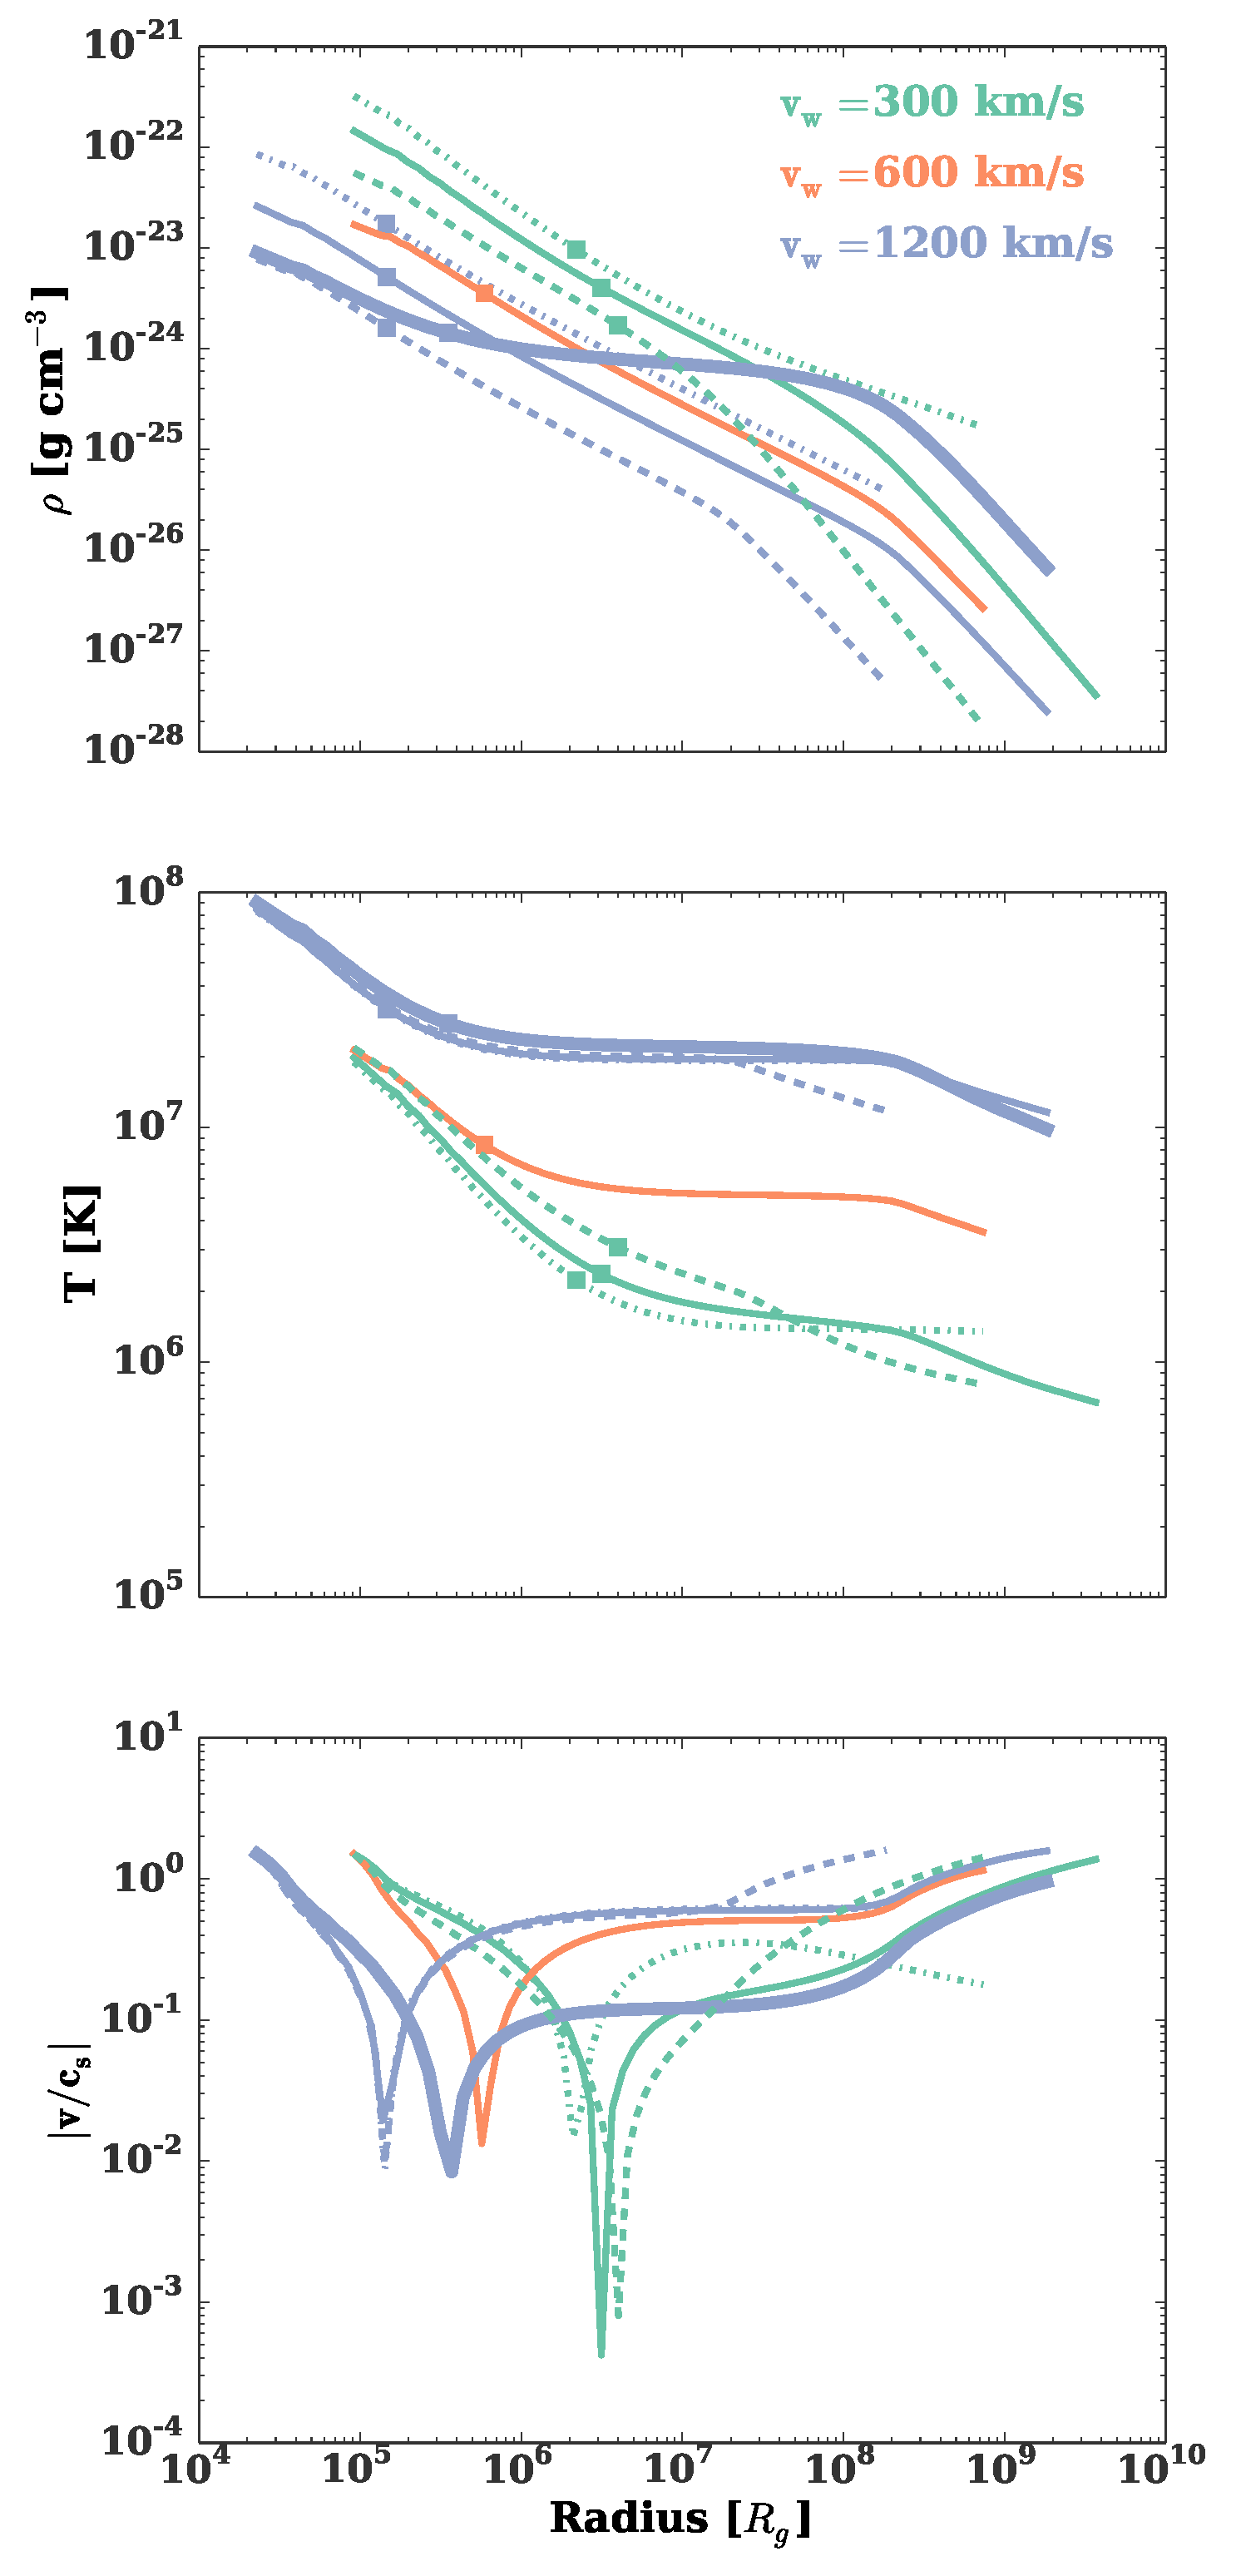
\includegraphics[width=\columnwidth]{profiles.eps}
  \caption{\label{fig:profiles}Radial profiles of the CNM density
    ({\it top}), temperature ({\it middle}), and velocity ({\it bottom}),
    calculated for a representative sample of galaxies.  Colors
    denote values of the effective wind heating rate,
    $\vwO=1200$ km s$^{-1}$ ({\it blue}), 600 km s$^{-1}$ ({\it
      orange}), and 300 km s$^{-1}$ ({\it green}).  Line styles denote different black hole masses: $\Mbh=10^6
    \Msun$ ({\it dot-dashed}), $10^7 \Msun$ ({\it solid}), and
    $10^8 \Msun$ ({\it dashed}). Thin and thick lines denote cusp galaxies ($\Gamma$=0.8) and core galaxies ($\Gamma$=0.1), respectively.  Squares mark the locations of the stagnation radius.
 }
\end{figure}

  \subsection{Angular Momentum}
  \label{sec:rotation}

  Our spherically symmetric model neglects the effects of angular
  momentum on the gas evolution.  However, all galaxies possess some
  net rotation, resulting in centrifugal forces becoming important at
  some radius $r_{\rm circ} = l^{2}_{s}/(GM_{\bullet})$.  Here
  $l_{s} = \langle r V_{\phi}\rangle |_{r_s}$ is the stellar
  specific angular momentum near the stagnation radius, from which
  most of the accreted mass originates, where $V_{\phi}$ is the
  stellar azimuthal velocity.

  \citet{EmsellemCappellari+:2007a} use two-dimensional kinematic data
  to measure the ratio of ordered to random motion in a sample of
  early type galaxies, which they quantify at each galactic radius $R$
  by the parameter
  \begin{align}
    \lambda_R \equiv \frac{\langle r|V|\rangle}{\langle R\sqrt{V^2+\sigma^2}\rangle} \underset{R \ll r_{\rm inf}}\sim \frac{V_{\phi}}{\sigma},
  \end{align}
  where $\sigma$ is the velocity dispersion and the brackets indicate
  a luminosity-weighted average.  The circularization radius of the
  accretion flow can be written in terms of $\lambda_R$ as

\begin{equation}
\frac{r_{\rm circ}}{r_{s}} \approx \frac{r_{s}}{r_{\rm inf}}\lambda_{R}^{2} \lesssim \lambda_{R}^{2},
\label{eq:rcirc}
\end{equation}
where we have used the definition $r_{\rm inf} \equiv
GM_{\bullet}/\sigma_{\bullet}^{2}$ and in the second inequality have assumed
that $r_{\rm s} \lesssim r_{\rm inf}$, a condition which is satisfied
for the thermally-stable solutions of interest.

\citet{EmsellemCappellari+:2007a} (their Fig.~2) find that $\lambda_R$
is generally $< 0.1$ on radial scales $<$ 10 per cent of the galaxy
half-light radius and that $\lambda_R$ decreases with decreasing $R$
interior to this point.  From equation (\ref{eq:rcirc}) we thus
conclude that $r_{\rm circ} \lesssim 0.01r_{s}$, i.e.~that gas will most likely
circularize within the inner sonic point of the flow (Fig.~\ref{fig:profiles}).  Angular momentum should only become
dynamically important for thermally stable flows in a region that is
causally disconnected from the outer part of the flow. Thus, the flow
properties on large scales will generally be unaffected by angular momentum.

%At $r\simeq r_{\rm circ} $ the gas will encounter a centrifugal
%barrier, which means that much of the gas flowing in from larger
%scales will be driven out in a conical outflow. \citep{Li+2013}
%suggest that the actual accretion rate will be $\sim\alpha$ times the
%accretion rate on large scales {\bf Note that new ending paragraph}.



\section{Numerical Results}
\label{sec:numerical}

\begin{table*}
\begin{threeparttable}
%\centering
\begin{minipage}{18cm}
  \caption{Summary of Numerical Solutions}
\begin{tabular}{lccccccccc}
  \hline
  {$M_{\bullet}$} & {$v_{w}$} & {$r_b^{(a)}$} &   $r_{\rm s}/r_{\rm
    inf}$ &  {$\left(\frac{\dot{M}}{\dot{M}_{\rm edd}}\right)_{r_{s}}^{(b)}
      (\eta=0.2)$} & {$\left(\frac{\dot{q}_{\rm heat}}{|\dot{q}_{\rm
            rad}|}\right)_{r_s}^{(c)} (\eta=0.2)$} & Unstable $\eta$'s  \\
    ($M_{\odot}$) & (km s$^{-1}$) & (pc) &- & - & - &  - & \\ 
    \hline
    Cusp Galaxies, $\Gamma = 0.8$ & & & & & & & & \\
    $    10^{ 6 }$ & 300 & -- & 0.12 & $ 5.1 \times 10^{ -5 }$ & 28 \\
    ... & 600 & -- & $ 3.2 \times 10^{ -2 }$ & $ 1.0 \times 10^{ -5 }$ & $ 1.9 \times 10^{ 3 }$ \\
    ... & 1200 & -- & $ 7.9 \times 10^{ -3 }$ & $ 1.8 \times 10^{ -6 }$ & $ 7.7 \times 10^{ 4 }$ \\
%    $    10^{ 7 }$ & 300 & 25 & 0.42 & $ 2.4 \times 10^{ -4 }$ & 7 & 0.2, 0.6\\ 
   10$^{7}$ & ... & 50 & 0.38 & $ 2.0 \times 10^{ -4 }$ & 4.5 & 0.2, 0.6\\
% ... & ... & 100 & 0.43 & $ 2.4 \times 10^{ -4 }$ & 2.7 & 0.2, 0.6 \\
% ... & ... & 200 & 0.47 & $ 2.7 \times 10^{ -4 }$ & $\mathbf{2.1}$ \\
% ... & ... & 400 & 1.1 & $ 7.0 \times 10^{ -4 }$ & $\mathbf{0.28}$ \\
... & ... & 100 & $\mathbf{TI}$ & $\mathbf{TI}$ & $\mathbf{TI}$ \\
... & ... & 200 & $\mathbf{TI}$ & $\mathbf{TI}$ & $\mathbf{TI}$ \\
... & ... & 400 & $\mathbf{TI}$ & $\mathbf{TI}$ & $\mathbf{TI}$ \\
... & 600 & 25 & $ 8.1 \times 10^{ -2 }$ & $ 3.2 \times 10^{ -5 }$ & $ 6.2 \times 10^{ 2 }$ \\
... & ... & 100 & $ 8.1 \times 10^{ -2 }$ & $ 3.2 \times 10^{ -5 }$ & $ 6.2 \times 10^{ 2 }$ \\
... & 1200 & 100 & $ 2.0 \times 10^{ -2 }$ & $ 6.0 \times 10^{ -6 }$ & $ 2.6 \times 10^{ 4 }$ \\
$    10^{ 8 }$ & 300 & 25 & 0.69 & $ 4.2 \times 10^{ -4 }$ & 5.5 & 0.6\\
... & ... & 50 & 0.92 & $ 6.0 \times 10^{ -4 }$ & 2 & 0.6\\
 ... & ... & 100 & 1.4 & $ 9.5 \times 10^{ -4 }$ & 0.48 & 0.2, 0.6 \\
 ... & ... & 200 & 2.5 & $ 1.9 \times 10^{ -3 }$ & $5.3 \times  10^{
   -2 }$ & 0.2, 0.6  \\
% ... & ... & 100 & $\mathbf{TI}$ & $\mathbf{TI}$ & $\mathbf{TI}$ \\
%... & ... & 200 & $\mathbf{TI}$ & $\mathbf{TI}$ & $\mathbf{TI}$ \\
... & 450 & 100 & 0.43 & $ 2.4 \times 10^{ -4 }$ & 19 \\
...$^{\dagger}$ & 450 & 100 & 1.2 & $ 8.1 \times 10^{ -4 }$ & 2.6 \\
... & 600 & 25 & 0.21 & $ 1.0 \times 10^{ -4 }$ & $ 2.1 \times 10^{ 2 }$ \\
... & ... & 100 & 0.22 & $ 1.1 \times 10^{ -4 }$ & $ 1.7 \times 10^{ 2
}$ \\
...$^{\dagger}$ & ... & 100 & 0.22 & $ 1.1 \times 10^{ -4 }$ & $ 1.6 \times 10^{ 2 }$ \\
...$^{\ddagger}$  & ... & 100 & 0.27 & $ 1.4 \times 10^{ -4 }$ & $ 1.3 \times 10^{ 2
}$ \\
... & ... & 200 & 0.23 & $ 1.1 \times 10^{ -4 }$ & $ 1.6 \times 10^{ 2 }$ \\
... & ... & 400 & 0.23 & $ 1.1 \times 10^{ -4 }$ & $ 1.5 \times 10^{ 2 }$ \\
... & 1200 & 100 & $ 5.0 \times 10^{ -2 }$ & $ 1.8 \times 10^{ -5 }$ & $ 8.3 \times 10^{ 3 }$ \\
\hline
Core Galaxies, $\Gamma = 0.1$  &  & & & & & & & & \\
$    10^{ 6 }$ & 600 & 25 & $ 9.4 \times 10^{ -2 }$ & $ 7.4 \times 10^{ -6 }$ & $ 1.1 \times 10^{ 2 }$ \\
... & 1200 & -- & $ 1.5 \times 10^{ -2 }$ & $ 2.3 \times 10^{ -7 }$ & $ 1.7 \times 10^{ 5 }$ \\
% ... & ... & 50 & $ 1.5 \times 10^{ -2 }$ & $ 2.3 \times 10^{ -7 }$ & $ 1.7 \times 10^{ 5 }$ \\
% ... & ... & 100 & $ 1.5 \times 10^{ -2 }$ & $ 2.3 \times 10^{ -7 }$ & $ 1.7 \times 10^{ 5 }$ \\
$    10^{ 7 }$ & 600 & 25 & 0.19 & $ 2.9 \times 10^{ -5 }$ & 79 & 0.6 \\
%... & ... & 50 & 0.76 & $ 3.9 \times 10^{ -4 }$ & $\mathbf{ 8.0
%\times 10^{ -2 }}$ \\
... & ... & 50 & $\mathbf{TI}$ & $\mathbf{TI}$ & $\mathbf{TI}$ \\
... & 1200 & 25 & $ 3.9 \times 10^{ -2 }$ & $ 1.4 \times 10^{ -6 }$ & $ 2.9 \times 10^{ 4 }$ \\
 ... & ... & 50 & $ 4.1 \times 10^{ -2 }$ & $ 1.5 \times 10^{ -6 }$ & $ 2.3 \times 10^{ 4 }$ \\
% ... & ... & 100 & $ 4.8 \times 10^{ -2 }$ & $ 2.1 \times 10^{ -6 }$ & $ 1.2 \times 10^{ 4 }$ \\
$    10^{ 8 }$ & 600 & 25 & 0.27 & $ 5.7 \times 10^{ -5 }$ & $ 1.0 \times 10^{ 2 }$ \\
... & ... & 50 & 0.46 & $ 1.5 \times 10^{ -4 }$ & 9.4 & 0.2, 0.6\\
... & 1200 & 25 & $ 8.5 \times 10^{ -2 }$ & $ 6.1 \times 10^{ -6 }$ & $ 8.2 \times 10^{ 3 }$ \\
... & ... & 50 & $ 9.2 \times 10^{ -2 }$ & $ 7.0 \times 10^{ -6 }$ & $ 6.0 \times 10^{ 3 }$ \\
... & ... & 100 & 0.1 & $ 8.8 \times 10^{ -6 }$ & $ 3.8 \times 10^{ 3 }$ \\
... & ... & 200 & 0.15 & $ 1.7 \times 10^{ -5 }$ & $ 8.0 \times 10^{ 2 }$ \\
% ... & ... & 400 & 0.8  & $ 2.5 \times 10^{ -2 }$ & $\mathbf{ 3.1 \times 10^{ -4 }}$ \\
\hline
\label{table:models}  
\end{tabular}
\begin{tablenotes}
\item $^{(a)}$ Break radius of stellar density profile.  $^{(b)}$Accretion
  rate in Eddington units, normalized to a stellar mass input
  parameter $\eta = 0.2$.  $^{(c)}$Ratio of wind heating rate to
  radiative cooling rate at the stagnation radius. $\dagger$Calculated with
  radiative cooling included, assuming mass loss parameter $\eta =
  0.2$.  $\ddagger$Calculated with radiative cooling and conductivity
  included, assuming mass loss parameter $\eta = 0.2$ and conductivity
  saturation parameter $\phi = 0.1$.  Solutions including radiative cooling were performed for cusp galaxies with $v_w=300 $ km s$^{-1}$ and core galaxies with $v_w=600 $ km s$^{-1}$ for $\eta$ = 0.02, 0.2, and 0.6.  Values of $\eta$ resulting in thermally unstable solutions are marked in the final column.  Solutions found to be thermally unstable for all $\eta
  \geq 0.02$ are denoted as {\bf TI}.
\end{tablenotes}
\end{minipage}
\end{threeparttable}

\end{table*}




%\begin{table*}
%\centering
%\begin{minipage}{18cm}
%\caption{Comparison of numerical solutions with and without
 % cooling. We have chosen $\eta=0.04$, which one would expect for 
  %the average star formation history for $\Mbh=10^8\Msun$ 
 % (see Figures~\ref{fig:eta} {\bf AG-cite star formation history
  %  figure once it is made.}). Note that we have deliberately chosen a solution
  %near our thermal stability threshold where cooling is beginning
  %to become important.
%}
%\begin{tabular}{lccccccccccccc}
%\hline
%{$M_{\bullet,8}$} & {$v_{w}$} & {$\Gamma$} & {$r_b$} & {$\eta$} &
%{$\dot{M}/\dot{M}_{\rm edd}$} & {$(t_{\rm cool}/t_{\rm ff})_{r_s}$} & {comments}\\
%\hline
%1 & 300 & 0.8 & 50.0 & 0.04 & $ 3.3 \times 10^{ -4 }$ & 4.6 &  \\
%1 & 300 & 0.8 & 50.0 & 0.04 & $ 9.1 \times 10^{ -4 }$ & 5.6 & \\
%\hline
%\label{table:models}  
%\end{tabular}
%\end{minipage}
%\end{table*}

Our numerical results, summarized in Table \ref{table:models}, allow
us to study a range of CNM properties and to assess the validity of
the analytic estimates from the previous section.  

Figure~\ref{fig:profiles} shows profiles of the density $\rho(r)$,
temperature $T(r)$, and radial velocity $|v(r)|/c_s$, for the cusp ($\Gamma=0.8$) solutions within our
grid.  As expected, the gas density increases towards the SMBH
$\rho\propto r^{-\densSlope}$ with $\densSlope\simeq1$, i.e. shallower
than the $-3/2$ power law for Bondi accretion. This power law behavior
does not extend through all radii, however, as the gas density profile
has a break coincident with the location of the break in the stellar
light profile ($\rb=100$ pc). The temperature profile is relatively
flat at large radii, but increases as $\propto 1/r^{k}$ interior to
the sphere of influence, where $k\lesssim 1$, somewhat shallower than
expected for virialized gas within the black hole sphere of influence.
The inwardly directed velocity increases towards the hole with a
profile that is somewhat steeper than the local free-fall velocity $v
\propto v_{\rm ff}\propto r^{-1/2}$.  The flow near the stagnation
radius is subsonic, but becomes supersonic at two critical points, one
located at small radii, $r \lesssim 0.1r_{\rm s}$, and the other
located at large radii, $r \gtrsim 10^{3}r_{\rm s}$.  In many cases
the outer supersonic transition is instigated by the transition to a steeper
stellar density profile exterior to the outer Nuker break radius.

Figure~\ref{fig:stag} shows our calculation of the stagnation radius
$r_{\rm s}/r_{\rm inf}$ as a function of the wind heating parameter
$\zeta = \sqrt{1+(v_w/\sigma_0)^{2}}$, with different colors
showing different values of $v_{w}$.  Cusp and core galaxies are
marked with square and triangles, respectively.  Shown for comparison
are our analytic results (eq.~[\ref{eq:rs2main}]) with solid and
dashed lines for cusp and core galaxies, respectively, calculated
assuming $\densSlope = 1$ and $\densSlope= 0.6$, respectively
(eq.~[\ref{eq:densSlope}]).

Our analytic estimates accurately reproduce the numerical results in
the high heating limit $\zeta \gg 1$ ($v_w \gg \sigma_0$; $r_{\rm s}
\lesssim r_{\rm inf}$).  However, for low heating the stagnation
radius diverges above the analytic estimate, approaching the stellar
break radius $r_b \gg r_{\rm inf}$.  This divergence occurs
approximately when $\zeta < \zeta_c \propto (r_b/r_{\rm
  soi})^{0.5(\Gamma-1)}$ (eq.~[\ref{eq:zetacrit}]), which coincides
with the Bernoulli parameter of the gas decreasing below unity near
the stagnation radius (Appendix \ref{app:be}).  Thus, for small values
of the heating rate (small $\zeta$) the location of the stagnation
radius will vary strongly with the break radius. This explains the
behavior of the three vertically aligned green squares. These are three
cusp ($\Gamma=0.8$) galaxies with $\Mbh=10^8 \Msun$ and $v_w=300$ km s$^{-1}$
but with different break radii ($\rb=$ 25, 50, and 100 pc from top to
bottom). This divergence of the stagnation radius to large radii
occurs at a higher value of $\zeta$ in core galaxies ($\Gamma = 0.1$),
explaining the behavior of the two core galaxies shown in
Fig.~\ref{fig:stag} as vertically aligned orange triangles.  
%These
%solutions correspond to the same black hole mass ($\Mbh = 10^8 \Msun$)
%and heating rate ($v_w = 600$ km s$^{-1}$) but assume different break
%radii of $r_{b} =$ 25, 50 pc (from top to bottom).

Figure~\ref{fig:mdot_mass} shows the SMBH accretion rate for a sample of
our numerical solutions for different values of
$\vwO =$ 300, 600 and 1200 km s$^{-1}$, and for both core
($\Gamma$=0.1) and cusp galaxies ($\Gamma$=0.8).  Shown for comparison
is our simple analytic estimate of $\dot{M}/\dot{M}_{\rm edd}$ from equation
(\ref{eq:eddr_analytic}).  For high wind velocities ($v_{w} \gg
\sigma_0$) the stagnation radius lies well inside the black hole sphere of
influence and our analytic estimate provides a good fit to the
numerical results.  However, for low wind velocities and/or high
$M_{\bullet}$ (large $\sigma_0$), the numerical accretion rate
considerably exceeds the simple analytic estimate as the stagnation radius
diverges to large radii (Fig.~\ref{fig:stag}).


\begin{figure}
  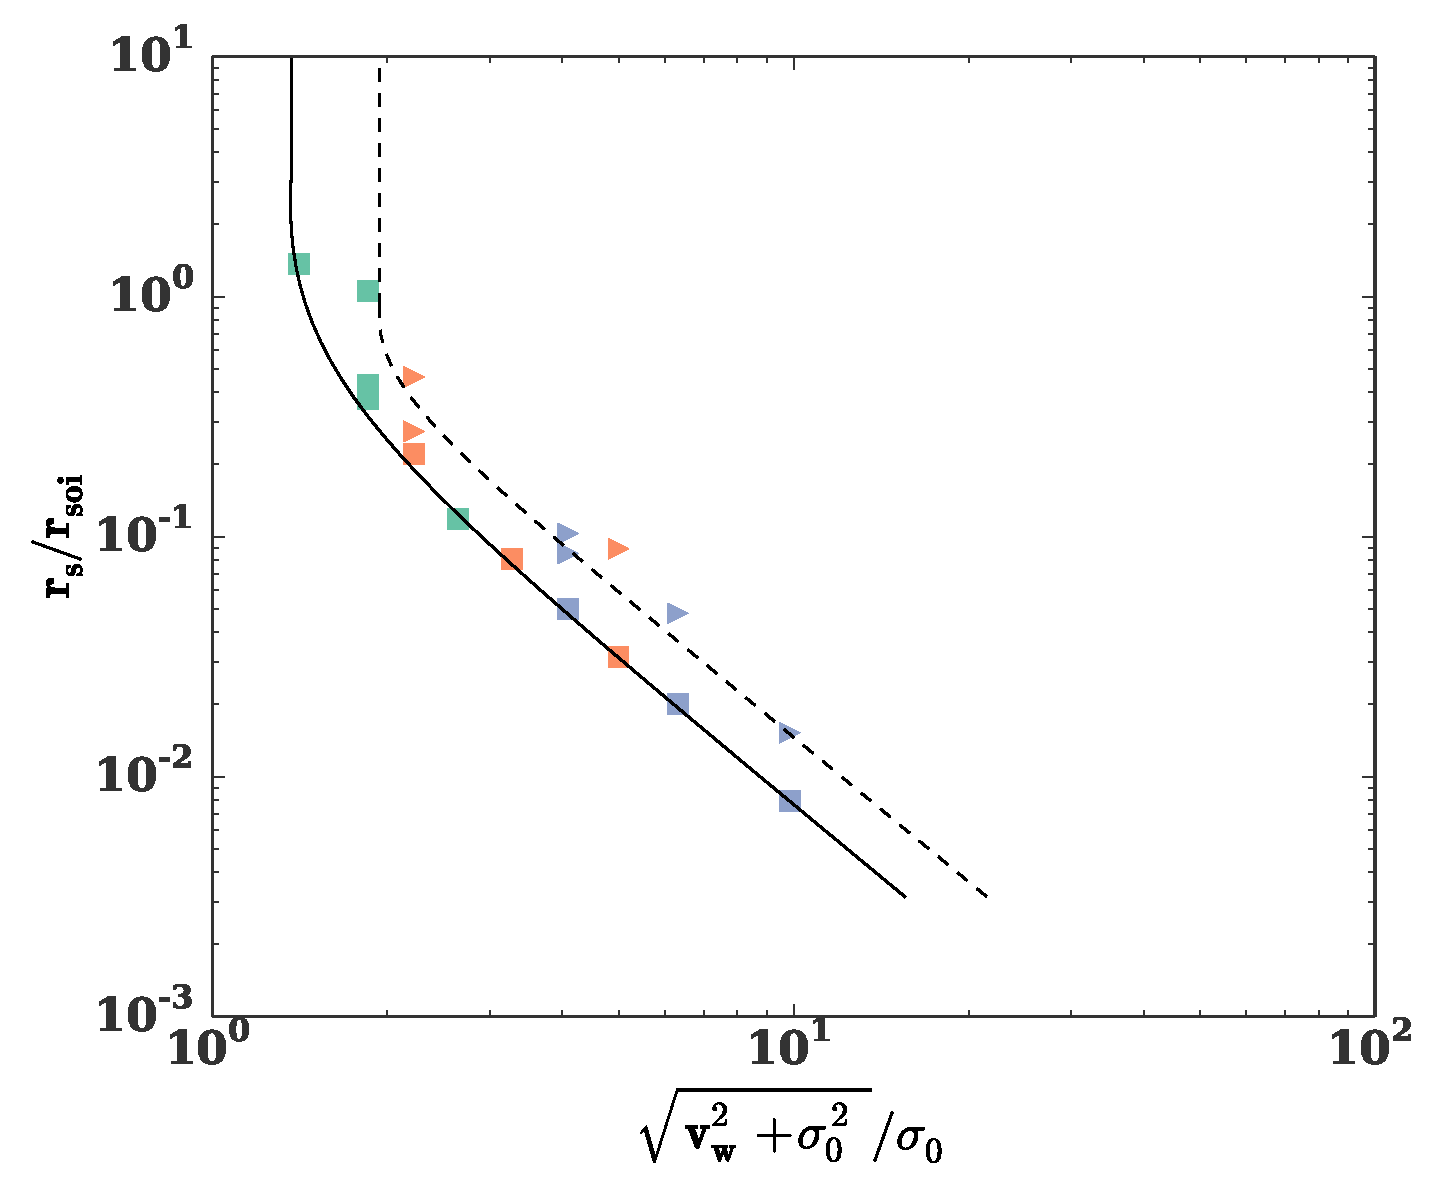
\includegraphics[width=\columnwidth]{rs.eps}
  \caption{\label{fig:stag} Stagnation radius $r_{s}$ in units of the
    sphere of influence radius $r_{\rm inf}$ (eq.~[\ref{eq:rsoi}]) for
    galaxies in our sample as a function of the stellar wind heating
    parameter $\zeta \equiv \sqrt{1+(v_w/\sigma_0)^{2}}$.  Green,
    orange, and blue symbols correspond to different values of $v_{w}
    =$ 300, 600, and 1200 km s$^{-1}$, respectively.  Squares
    correspond to cusp galaxies ($\Gamma = 0.8$), while triangles
    correspond to cores ($\Gamma = 0.1$). Green circles correspond to
    cusp solutions which would be thermally unstable.  The black
    curves correspond to the analytic prediction from equation
    (\ref{eq:rs2main}), with thick solid and dot-dashed curves
    calculated for parameters $(\Gamma=0.8, \densSlope\simeq 1)$ and
    $(\Gamma=0.1,\densSlope\simeq0.6)$, respectively. The thin black
    solid line corresponds to the simplified analytic result for $\rs$
    from equation~\eqref{eq:stag_simple} (recall that $\rinf \simeq 14
    \Mbheight^{0.6} {\rm pc}$).}
\end{figure}

\begin{figure}
  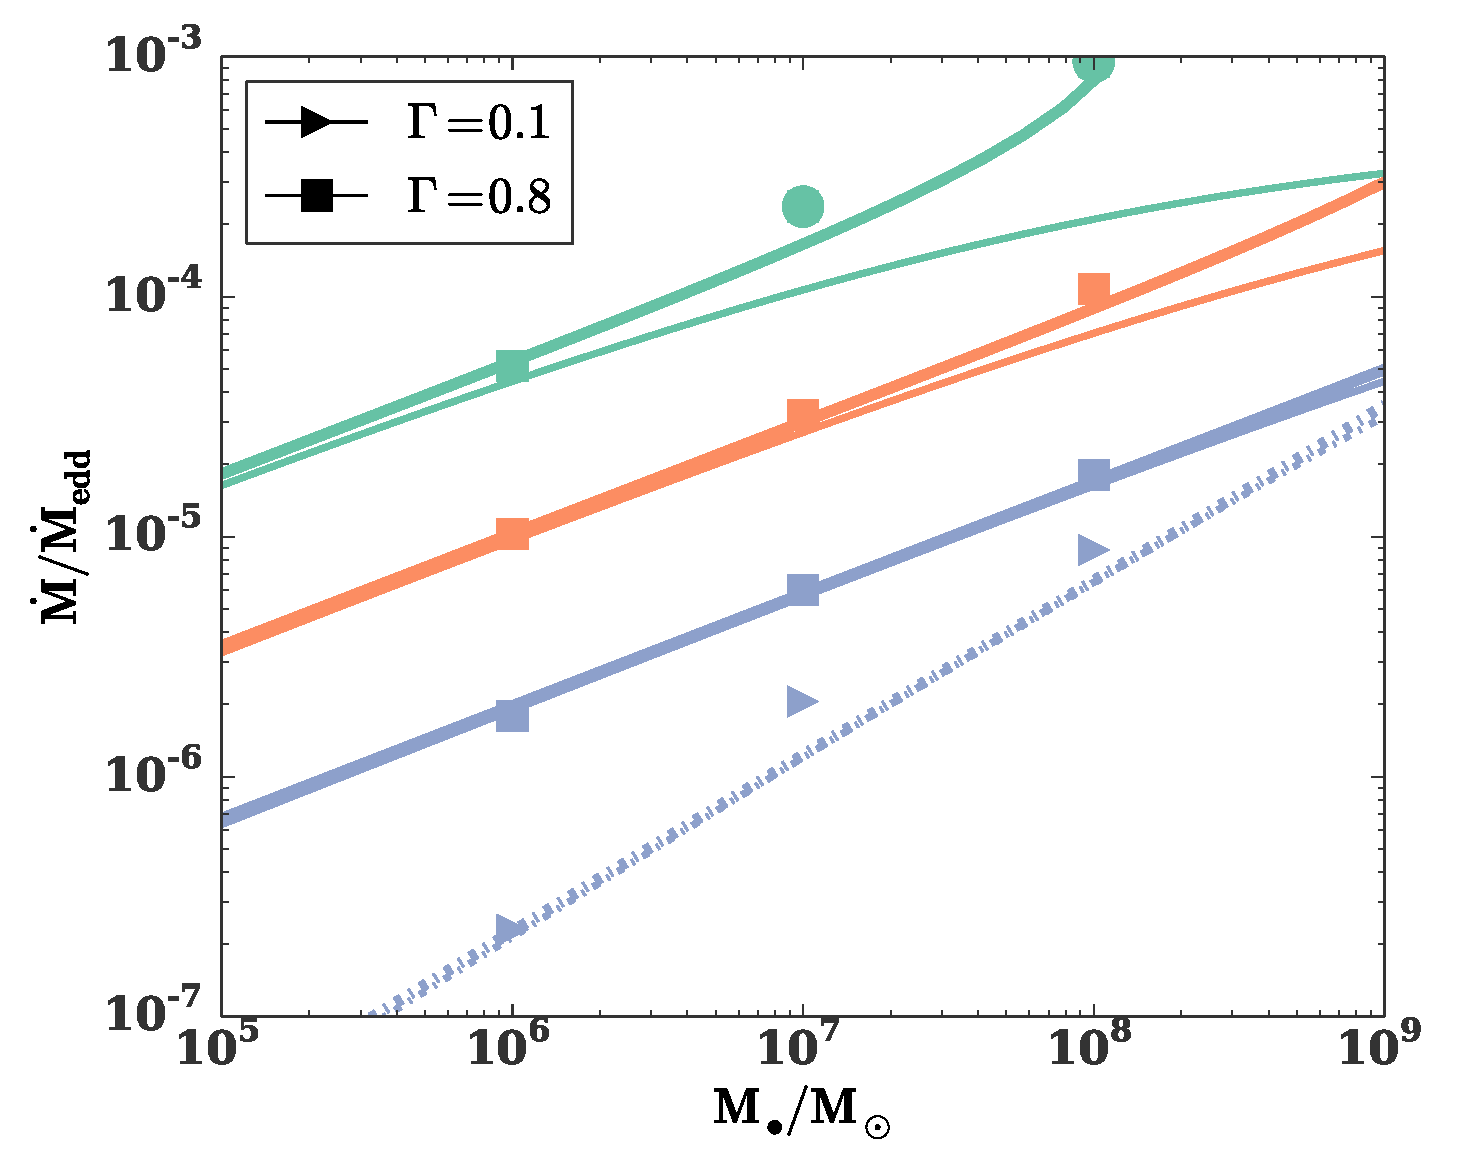
\includegraphics[width=\columnwidth]{mdot_mass.eps}
  \caption{\label{fig:mdot_mass} Accretion rate $\dot{M}/\dot{M}_{\rm
      edd}$ versus SMBH mass for galaxies in our sample, calculated
    for different values of the wind heating parameter $\vwO =$ 300 km
    s$^{-1}$ ({\it green}), 600 km s$^{-1}$ ({\it orange}), and 1200
    km s$^{-1}$ ({\it blue}).  Squares correspond to cusp galaxies
    ($\Gamma=0.8$), while triangles correspond to cores
    ($\Gamma$=0.1). Green circles correspond to cusp solutions which
    would be thermally unstable.  Thin solid and dot-dashed curves
    correspond to our simple analytic estimates of $\dot{M}/\dot{M}_{\rm
      edd}$ (eq.~[\ref{eq:eddr_analytic}]) for cusp and core galaxies,
    respectively.  Thick curves correspond to the more accurate implicit analytic expression given by equation \eqref{eq:rs2main}.}
\end{figure}


\begin{figure}
  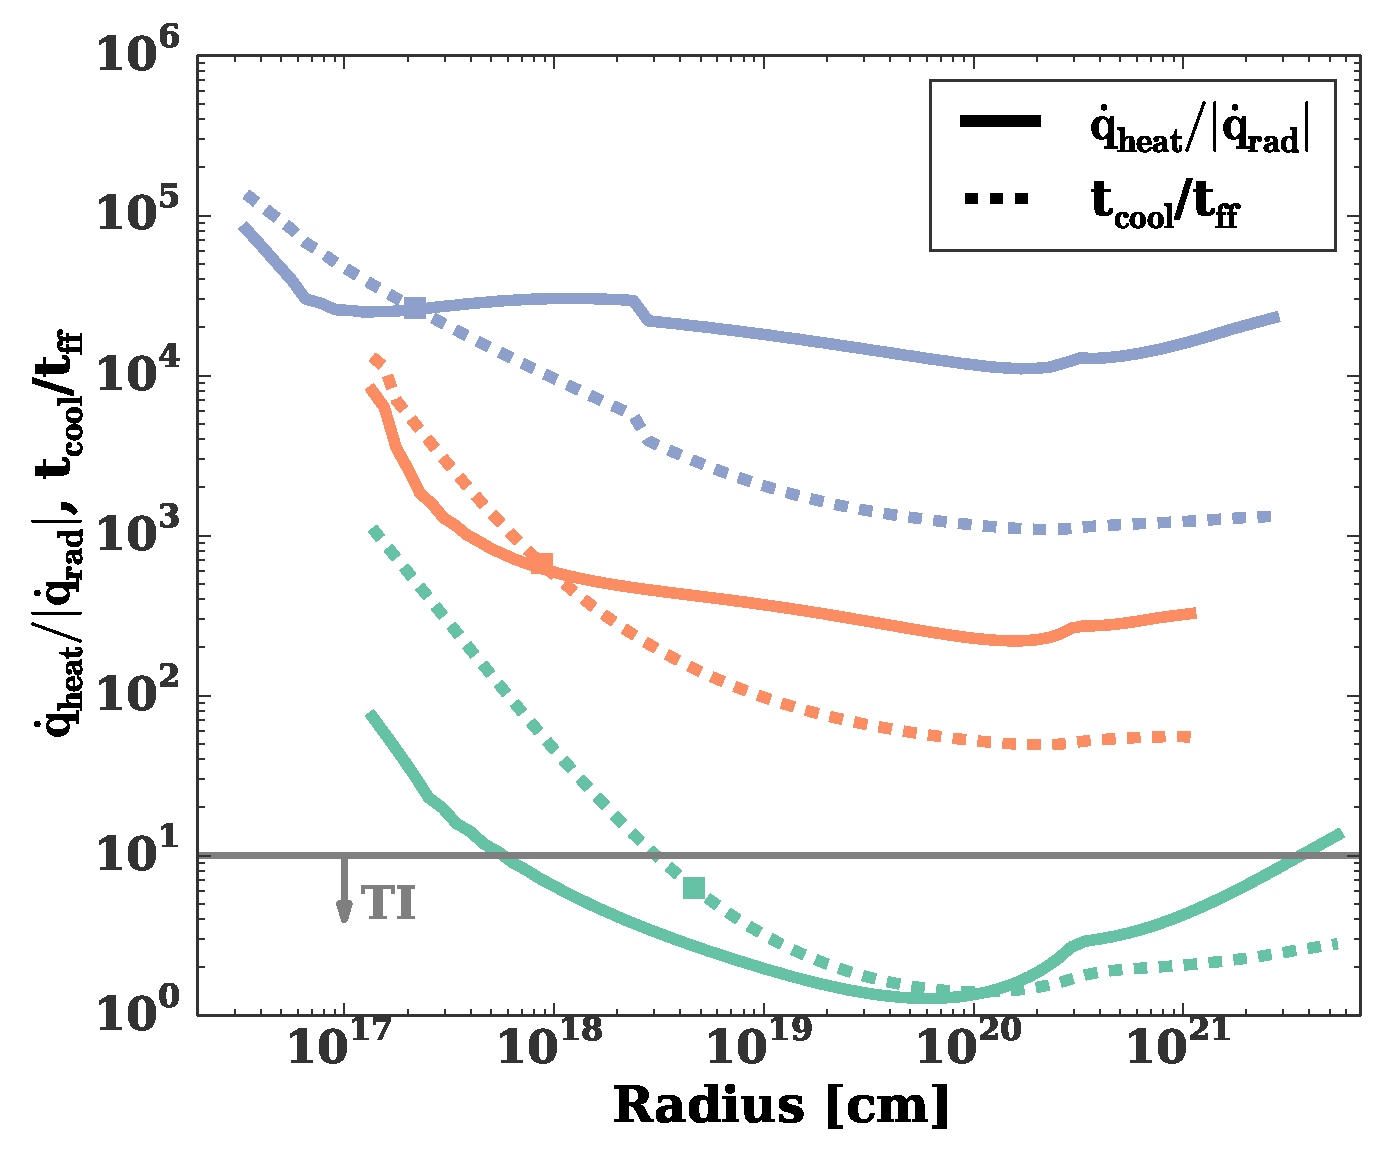
\includegraphics[width=\columnwidth]{cooling.eps}
  \caption{\label{fig:cooling} Ratio of the rates of heating to
radiative cooling, $\dot{q}_{\rm heat}/|\dot{q}_{\rm rad}|$, as a
function of radius (solid lines) for each of our solutions shown in
Figure \ref{fig:profiles}.  Dashed lines show the ratio
of the cooling timescale to the free-fall timescale $t_{\rm cool}/t_{\rm ff}$.
For high heating rates both ratios are approximately equal at the
stagnation radius (squares).  When $\dot{q}_{\rm
heat}/\dot{q}_{\rm rad} \lesssim 10$ (or, equivalently, $t_{\rm cool}/t_{\rm ff}
\lesssim 10$ near the stagnation radius), then the flow is susceptible to thermal instabilities.}
\end{figure}


Fig.~\ref{fig:cooling} shows the ratio of wind heating to radiative
cooling, $\dot{q}_{\rm heat}/|\dot{q}_{\rm rad}|$
(eq.~[\ref{eq:cooling2}] and surrounding discussion) as a function of
radius for our fiducial solutions shown in Figure \ref{fig:profiles}.
Radiative cooling is calculated using the cooling function of \citet{Draine:2011a} for solar metallicity.  For high heating rates of $v_{w} = 600$ and
$1200$ km s$^{-1}$ cooling is unimportant across all radii, while for
$v_{w} = 300$ km s$^{-1}$ we see that $\dot{q}_{\rm
  heat}/|\dot{q}_{\rm rad}|$ and $\tcool/\tff$ can be less than unity,
depending on the wind mass loss parameter $\eta$.  Because at the
stagnation radius $\dot{q}_{\rm heat}/|\dot{q}_{\rm rad}|$ reaches
within a factor of two of its minimum across the entire grid, the
value of $(\dot{q}_{\rm heat}/|\dot{q}_{\rm rad}|)_{r_{s}}$ can be
taken as diagnostic of thermal instability at all radii.

Also note that for $v_{w}=600$ and $1200$ km s$^{-1}$ we have $\dot{q}_{\rm heat}/|\dot{q}_{\rm rad}| \sim t_{\rm cool}/t_{\rm ff}$
near the stagnation radius, but these ratios diverge from each other at low heating ($v_{w} \lesssim 300$ km s$^{-1}$).  This results because equations (\ref{eq:mdot_gas}), (\ref{eq:rhors}) underestimate the true gas density in the case of subsonic flow (weak heating).

Although most of our solutions neglect thermal conduction and
radiative cooling, these effects are explore explicitly in subset of simulations, as marked by dagger symbols in Table \ref{table:models}.  For cases which are far from being thermally
unstable when cooling is neglected (e.g., $M_{\bullet} =
10^{8}M_{\odot}$, $v_{w} = 600$ km s$^{-1}$, $r_{b} = 100$ pc, $\eta =
0.2$, $\dot{q}_{\rm heat}/|\dot{q}_{\rm rad}| = 76$), including radiative cooling has little effect on the key properties of the solution, such as the stagnation radius, mass accretion rate, and the cooling ratio $\dot{q}_{\rm
  heat}/|\dot{q}_{\rm rad}|$.  However, for solutions that are marginally thermally stable, including radiative losses acts to significantly decrease $\dot{q}_{\rm heat}/|\dot{q}_{\rm rad}|$.  We calculated solutions with radiative
cooling for all cusp galaxies with $v_w=300$ km s$^{-1}$ and for all
core galaxies with $v_w=600 $ km s$^{-1}$, each for three different
values of $\eta = 0.02, 0.2, 0.6$, spanning the physical range of
expected mass loss for continuous star formation (Fig.~\ref{fig:vwSources}).  Solutions found to be unstable for all values of $\eta$ are marked in boldface as ``TI" in Table
\ref{table:models}, with the unstable values of $\eta$ provided in the final column.

Including thermal conduction, by contrast, results in only minor changes to our solutions for our fiducial value of the saturation parameter $\phi = 0.1$, consistent with our analytic expectation (eq.~[\ref{eq:conduction}]).  

\section{Heating Sources}
\label{sec:heating}

Key properties of the flow, such as the SMBH accretion rate and the likelihood of thermal instability depend sensitively on the assumed heating rate $\propto qv_{w}^{2}$.  This section summarizes individual heating sources, providing estimates of the value of
\begin{align}
  v_{w} = \sqrt{\frac{2 t_h \dot{e}}{\eta \rhostar}}
  \label{eq:vw_eff}
\end{align}
for each, where $\dot{e}$ is volumetric heating rate.  

\subsection{Stellar winds} 

Energy and mass input to the CNM by stellar winds is the sum of contributions from main sequence and post-main sequence populations.  At early times following star formation, energy input is dominated by core collapse supernovae and by the fast outflows of Wolf-Rayet stars (e.g., \citealt{VossDiehl+:2009a}).  At later times energy input is dominated by main sequence winds (e.g., \citealt{NaimanSoares-Furtado+:2013a}).  Mass input is also dominated by massive stars for very young stellar populations, but for most stellar ages the slow AGB winds of evolved low-mass stars dominate the mass budget.  

In Appendix \ref{app:windheat} we calculate the wind heating rate from
stellar winds, $v_{\rm w}^{\star}$, and the mass loss parameter,
$\eta$ (eq.~[\ref{eq:q}]), as a function of age, $\tau_{\star}$, of a
stellar population which is formed impulsively (Fig.~\ref{fig:vwImp}).  
At the earliest times ($\tau_{\star} \lesssim 10^{7}$ yr), the wind
heating rate exceeds 1000 km s$^{-1}$, while much later ($\tau_{\star}
\sim t_{\rm h}$) stellar wind heating dominated by main sequence winds
is much lower, $v^{\star}_{\rm w} \sim 50-100 $ km s$^{-1}$.  As will be shown in $\S\ref{sec:combined}$, for the case of quasi-continuous star
formation representative of the average SFHs of low
mass galaxies, the heating rate from stellar winds can also be significant, $v_{\rm w}^{\star} \sim 1000$ km s$^{-1}$.  

Stellar winds thus contribute a potentially important source of both
energy and mass to the CNM.  However, two additional uncertainties are (1) the efficiency with which massive stellar winds thermalize their energy and (2) heating from core collapse supernovae, which is potentially comparable to that provided by stellar winds.  We neglect both effects, but expect they will act in different directions in changing the total heating rate.  

\subsection{Type Ia Supernovae} 

Type Ia SNe represent a source of heating, which unlike core collapse
SNe is present even in an evolved stellar population.  If each SN Ia
injects thermal energy $E_{\rm Ia}$ into the interstellar medium, and
the SN rate per stellar mass is given by $R_{\rm Ia}$, then the
resulting volumetric heating rate of $E_{\rm Ia}R_{\rm Ia}$ produces
an effective heating parameter (eq.~[\ref{eq:vw_eff}])
of \begin{align} v_{w}^{\rm Ia} =\sqrt{\frac{2 t_h R_{\rm Ia} E_{\rm
        Ia}}{\eta}} \label{eq:vw_sne}.
\end{align} The thermal energy injected by each SN Ia, $E_{\rm Ia} \simeq
\epsilon_{\rm Ia} 10^{51}$ erg, depends on the efficiency $\epsilon_{\rm Ia}$
with which the initial blast wave energy is converted into bulk or turbulent
motion instead of being lost to radiation.  \cite{Thornton+98}
estimate a radiative efficiency $\epsilon_{\rm Ia} \sim 0.1$,
depending weakly on surrounding density, but \citet{Sharma+14} argues
that $\epsilon_{\rm Ia}$ can be considerably higher, $\sim 0.4$, if
the SNe occur in a hot dilute medium, as may characterize the CNM.  Hereafter we adopt $\epsilon_{\rm Ia} = 0.4$ as fiducial.

The SN Ia rate, $\RateIa$, depends on the age of the stellar
population, as it represent the convolution of the star formation rate
and the Ia delay time distribution (DTD) divided by the present
stellar mass.  In the limit of impulsive star formation, $\RateIa$ is
the DTD evaluated at the time since the star formation episode.  The
observationally-inferred DTD (Fig. 1 of \citealt{MaozMannucci+:2012a})
has the approximate functional form \begin{align} R_{\rm Ia}
  =1.7\times 10^{-14}\left(\tau_{\star}/t_{\rm h}\right)^{-1.12}
  M_{\odot}^{-1}\,{\rm yr^{-1}}
\label{eq:DTD}
  \end{align}
  where $\tau_{\star}$ is the time since star formation.

From equations (\ref{eq:vw_sne}), (\ref{eq:DTD}) we thus estimate that 
  \begin{eqnarray} 
    v_{w}^{\rm Ia} &\approx& 700(\epsilon_{\rm
      Ia}/0.4)^{0.5}(\tau_{\star}/t_{\rm h})^{-0.56}\eta_{0.02}^{-1/2}\,{\rm km
      \,s^{-1}} \nonumber \\
&\approx& 700(\epsilon_{\rm
      Ia}/0.4)^{0.5}(\tau_{\star}/t_{\rm h})^{0.09}\,{\rm km
      \,s^{-1}},
\label{eq:vIa}
  \end{eqnarray}
  where the second line assumes $\eta\simeq 0.02
  (\tau_{\star}/t_h)^{-1.3}$ for a single burst of star formation
  (e.g. , \citealt{Ciotti+91}).

The high value of $v_{w}^{\rm Ia}$ implies that Ia SNe represent an
important source of CNM heating.  However, SNe can only be
approximated as supplying heating which is spatially and temporally
homogeneous if the rate of SNe is rapid compared to the characteristic
evolution time of the flow at the radius of interest
(\citealt{ShcherbakovWong+:2014a}).  We define the ``Ia radius"
  \begin{align}
    r_{\rm Ia} \sim \left(\frac{G}{R_{\rm Ia}\sigma_0}\right)^{1/2} \sim
    35 M_{\bullet,8}^{-0.1}(\tau_{\star}/t_{\rm h})^{0.56}\,{\rm pc}
    \label{eq:rIa}
  \end{align}
  as the location exterior to which the time interval between
  subsequent supernovae $\tau_{\rm Ia} \sim (M_{\rm enc}R_{\rm
    Ia})^{-1} \sim G/(r\sigma_0^{2}R_{\rm Ia})$ exceeds the local
  dynamical timescale $t_{\rm dyn} \sim r/\sigma_0$, where we again
  adopt the Ia rate for an old stellar population and in the final
  equality we estimate $\sigma_0 \approx \sqrt{3}\sigma_{\bullet}$
  using $M_{\bullet}-\sigma$ (eq.~[\ref{eq:Msigma}]).

Assuming that $v_{w}^{\rm Ia} \gg \sigma_0$ then by substituting
$v_{w}^{\rm Ia}$ (eq.~\ref{eq:vIa}) into equation (\ref{eq:stag_simple})
for the stagnation radius, we find that
\begin{align}
  \left.\frac{r_{\rm Ia}}{r_{\rm s}}\right|_{\rm v_{w}^{\rm Ia}}&\approx
  \begin{cases}
    7\, \eta_{0.02}^{-1} M_{\bullet,8}^{-1.1}(\epsilon_{\rm
     Ia}/0.4) (\tau_{\star}/t_{\rm h})^{-0.56}  & {\rm core}\\
    14\, \eta_{0.02}^{-1} M_{\bullet,8}^{-1.1}(\epsilon_{\rm
     Ia}/0.4) (\tau_{\star}/t_{\rm h})^{-0.56} &{\rm cusp}\\
   \end{cases} \nonumber\\
 &\approx 
 \begin{cases}
    7\, M_{\bullet,8}^{-1.1}(\epsilon_{\rm
     Ia}/0.4) (\tau_{\star}/t_{\rm h})^{0.74}  & {\rm core}\\
    14\, M_{\bullet,8}^{-1.1}(\epsilon_{\rm
     Ia}/0.4) (\tau_{\star}/t_{\rm h})^{0.74} &{\rm cusp}\\
   \end{cases}
\label{eq:rIars}
\end{align}
SN Ia can only be approximated as a steady heating source near the stagnation radius for extremely
massive SMBHs with $M_{\bullet} \gtrsim 10^9 \Msun$ or for a very
young stellar population with $\tau_{\star} \ll t_{\rm h}$.

Even if SN Ia are rare near the stagnation radius, they may cap the
SMBH accretion rate by periodically blowing gas out of the nucleus of
low mass galaxies.  Between successive SNe, stars release a gaseous
mass $M_{\rm g} \approx \eta M_{\star}\tau_{\rm Ia}/t_{\rm h}$
interior to the Ia radius, which is locally gravitationally bound to
the SMBH by an energy $E_{\rm bind} \gtrsim M_{\rm g}\sigma_0^{2}$.
From the above definitions it follows that \be \frac{E_{\rm
    Ia}}{E_{\rm bind}} \lesssim \frac{(v_{w}^{\rm
    Ia})^{2}}{2\sigma_0^{2}}.
\label{eq:blowout}
\ee
Hence, for low mass BHs with $\sigma_0 \ll v^{\rm Ia}_{w}$, SN Ia are capable of dynamically clearing out gas from radii $\sim r_{\rm Ia} \gtrsim r_{\rm s}$.  Thus even when heating is sufficiently weak that the stagnation radius formally exceeds $r_{\rm Ia}$, the SMBH accretion rate is still limited to a value
\begin{eqnarray}
\frac{\dot{M}_{\rm Ia}}{\dot{M}_{\rm edd}} &\approx& \frac{\eta M_{\bullet}}{\dot{M}_{\rm edd} t_{\rm h}}\left(\frac{r_{\rm Ia}}{r_{\rm inf}}\right)^{2-\Gamma} \approx \nonumber \\
 && \begin{cases}
    4.5 \times 10^{-4} M_{\bullet,8}^{-1.33}(\tau_{\star}/t_{\rm h})^{-0.2}
   & \text{core} \\
    2.2 \times 10^{-4} \Mbheight^{-0.84}(\tau_{\star}/t_{\rm h})^{-0.6}   & \text{cusp},
  \end{cases}
  \label{eq:eddr_Ia}
\end{eqnarray}
obtained substituting the Ia radius $r_{\rm Ia}$ (eq.~[\ref{eq:rIa}])
for $r_{\rm s}$ in the derivation leading to our estimate of $\dot{M}$
(eq.~[$\ref{eq:eddr_analytic}$]).  
%Note, however, that for low mass
%SMBHs, $\dot{M}_{\rm Ia}$ generally exceeds the maximum accretion rate
%for a thermally stable flow $\dot{M}_{\rm TI}$
%(eq.~[\ref{eq:Mdotmax}]), implying that dynamical `blow-out' from SNe
%Ia cannot alone prevent cooling instabilities in the nuclei of low
%mass galaxies.

The deep gravitational potential wells of high mass galaxies prevent SN Ia from dynamically clearing out gas in these systems ($\sigma_0 \gg  v^{\rm Ia}_{w}$).  Equation (\ref{eq:eddr_Ia}) nevertheless still represents a cap on the accretion rate in practice because the Ia heating rate (eq.~[\ref{eq:vIa}])
is usually high enough to prevent the stagnation radius (calculated including the Ia heating) from substantially exceeding $r_{\rm Ia}$. If the stagnation radius moves inwards from $\rIa$, then decreased heating will force it outwards again.  On the other hand, if the stagnation radius moves well outside of $\rIa$, then the high level of Ia heating will force it inwards. 

%Finally, note that our criterion for cooling instability (eq.~[\ref{eq:cooling2}], [\ref{eq:Mdotmax}]) is no longer valid if $\rs$ is regulated to $\rIa$ instead of being determined by equation \eqref{eq:stag_simple}.  By re-evaluating the density and temperature of gas at $\rIa$ using equations  (\ref{eq:rhors2}) and (\ref{eq:Tanalytic}) for $v_w = v_{w}^{\rm Ia}$, we find that
%\begin{align}
%\label{eq:heatingratioIa}
%&\left.\frac{\dot{q}_{\rm heat}}{\left|\dot{q}_{\rm rad}\right|}\right|_{\rIa}\simeq
%\begin{cases}
 % 90 \Mbheight^{1.3} (\epsilon_{\rm Ia}/0.4)^{1.7} (\tau_{\star}/\th)^{-3}
  %\eta_{0.02}^{-2.7} & \text{core}\nonumber\\
   %90 \Mbheight^{0.8} (\epsilon_{\rm Ia}/0.4)^{1.7} (\tau_{\star}/\th)^{-2.7}
  %\eta_{0.02}^{-2.7} & \text{cusp}\nonumber\\
%\end{cases}\\&\simeq
%\begin{cases}
 % 90 \Mbheight^{1.3} (\epsilon_{\rm Ia}/0.4)^{1.7}
  %(\tau_{\star}/\th)^{0.5}
 %& \text{core}\\
  % 90 \Mbheight^{0.8} (\epsilon_{\rm Ia}/0.4)^{1.7} (\tau_{\star}/\th)^{0.9}
  %& \text{cusp}\\
%\end{cases}
%\end{align}
%For high mass galaxies and relatively old stellar populations, Ia heating can preventing cooling instabilities on scales of the stagnation radius, i.e. $(\dot{q}_{\rm heat}/|\dot{q}_{\rm rad}|)_{\rIa} \gtrsim 10$.  However, for lower mass galaxies or younger stellar populations, Ia blow-out cannot prevent cooling instabilities.


%Also note that Ia supernovae only cap the accretion rate to this maximum value if the gas feeding the black hole is supplied by local stellar mass loss: the gaseous mass can become much greater if the nucleus is fed externally, e.g. due to a galaxy merger or to cooling flows developing within the galaxy over much longer timescales (e.g.~\citealt{Ciotti&Ostriker07}). 



\subsection{Millisecond Pulsars}
Energy injection from the magnetic braking of millisecond pulsars
(MSPs) is a potentially important heating source.  If the number of
MSPs per unit stellar mass is $n_{\rm msp}$ and each contributes on
average a spin-down luminosity $\bar{L}_{\rm sd}$, then the resulting
heating per unit volume $\dot{e} \approx \bar{L}_{\rm sd}n_{\rm
  msp}\epsilon_{\rm msp}$ results in an effective heating rate (eq.~
[\ref{eq:vw_eff}]) of
\begin{eqnarray} v_{w}^{\rm MSP} \sim
30\left(\frac{\epsilon_{\rm msp}}{0.1}\right)^{1/2}\left(\frac{\bar{L}_{\rm
sd}}{10^{34}\,{\rm erg\,s^{-1}}}\right)^{1/2} \eta_{0.02}^{-1/2}\,{\rm
km\,s^{-1}},
 \label{eq:vmsp}
  \end{eqnarray} 
  where $\epsilon_{\rm msp}$ is the thermalization efficiency of the
  wind, normalized to a value $\lesssim 0.1$ based on that inferred by
  modeling the interstellar media of globular clusters
  \citep{NaimanSoares-Furtado+:2013a}.  Our numerical estimate assumes
  a pulsar density $n_{\rm msp} \sim 3 \times 10^{-40} $ MSPs
  g$^{-1}$, calculated from the estimated $\sim 30,000$ MSPs in the
  Milky Way (\citealt{Lorimer13}) of stellar mass $\approx 6\times
  10^{10}M_{\odot}$.

  Based on the ATNF radio pulsar catalog (\citealt{Manchester+05}), we
  estimate the average spin-down luminosity of millisecond pulsars in
  the field to be $\bar{L}_{\rm sd} \sim 10^{34}$ erg s$^{-1}$,
  resulting in $v_{w}^{\rm MSP} \lesssim 30$ km s$^{-1}$ for $\eta
  \gtrsim 0.02$.  For higher spin-down luminosities, $L_{\rm sd}\simeq
  10^{35}$ ergs s$^{-1}$ characteristic of some Fermi-detected
  pulsars, then the higher value of $v_{w}^{\rm MSP} \lesssim 300$ km
  s$^{-1}$ makes MSP heating in principle important under the most
  optimistic assumptions $\epsilon_{\rm msp} = 1$ and $\eta = 0.02$.
%  On the other hand, it seems likely that the stellar binaries giving rise to MSPs could be disassociated by stellar interactions in the dense nuclear cluster, reducing the numbers of MSPs as compared to the field population estimate above.  


\subsection{SMBH Feedback}

Feedback from accretion onto the SMBH represents an important source of heating which, however, is also the most difficult to quantify (e.g., \citealt{Brighenti&Mathews03}, \citealt{DiMatteo+05}; \citealt{Kurosawa&Proga09}; \citealt{Fabian12} for a recent review).  A key difference between AGN heating and the other sources discussed thus far is its dependence on the SMBH accretion rate $\dot{M}$, which is itself a function of the heating rate (eq.~[\ref{eq:mdot_analytic}]).  

\subsubsection{Compton Heating}

There are two types of SMBH feedback: kinetic and radiative.
Radiative feedback is potentially effective even in low luminosity AGN
via Compton heating (e.g., \citealt{Sazonov+04}, \citealt{Ciotti+10}),
which provides a volumetric heating rate (\citealt{Gan+14})
\begin{align}
\dot{e} = 4.1\times 10^{-35}n^{2}\xi T_{\rm C}\,{\rm erg\,cm^{-3}\,s^{-1}},
\end{align}
where $\xi = L/n r^{2}$ is the ionization parameter and $L$ is the SMBH luminosity with Compton temperature $T_{\rm C} \sim 10^{9}$ K $\gg T$ (e.g., \citealt{Ho99}, \citealt{Eracleous+10}).  

The importance of Compton heating can be estimated by assuming the
SMBH radiates with a luminosity $L = \epsilon \dot{M}c^{2}$, where
$\epsilon$ is the radiative efficiency and where $\dot{M}$ is
estimated from equation (\ref{eq:mdot_analytic}).  Then using
equations (\ref{eq:stag_simple}), (\ref{eq:mdot_analytic}),
(\ref{eq:rhors}), (\ref{eq:rhostarrs}) we calculate from equation
(\ref{eq:vw_eff}) that the effective heating rate at the stagnation
radius is given by
\begin{align} v_{w}^{\rm C} \simeq
  \begin{cases} 24 \eta_{0.02}^{0.5}T_{\rm
C,9}^{0.5}\epsilon_{-2}^{0.5} M_{\bullet,8}^{0.38}v_{500}^{-1.4}\,{\rm
km\,s^{-1}} &, \text{core}\\ 30 \eta_{0.02}^{0.5}T_{\rm
C,9}^{0.5}\epsilon_{-2}^{0.5} M_{\bullet,8}^{0.24}v_{500}^{-0.7}\,{\rm
km\,s^{-1}} &, \text{cusp},
  \end{cases}
  \label{eq:vC}
\end{align} where $T_{C,9} = T_{C}/10^{9}$ K and $\epsilon_{-2} =
\epsilon/0.01 \sim 1$.  We caveat that, unlike stellar wind heating,
Compton heating depends on radius, scaling as $v_{w}^{\rm C}(r)
\propto (n^{2}\xi/\rho_{\star})^{1/2} \propto
r^{(\Gamma-\densSlope-1)/2}$, i.e. $\propto r^{-0.6}$ and $\propto
r^{-0.75}$ for core ($\Gamma = 0.8$; $\densSlope \simeq 1$) and cusp
($\Gamma = 0.1$; $\densSlope \simeq 0.6$) galaxies, respectively.
Although our model's assumption that the heating parameter be radially
constant is not satisfied, this variation is sufficiently weak that it
should not significantly alter our conclusions.

If Compton heating acts alone, i.e. $\tilde{v}_{w} = v_{w}^{C}$, then
solving equation (\ref{eq:vC}) for $\tilde{v}_{\rm w}$ yields
\begin{align} v_{w}^{\rm C} \simeq
  \begin{cases} 140 \eta_{0.02}^{0.21}T_{\rm
C,9}^{0.21}\epsilon_{-2}^{0.21} M_{\bullet,8}^{0.16}\,{\rm km\,s^{-1}}
&, \text{core}\\ 95 \eta_{0.02}^{0.34}T_{\rm
C,9}^{0.29}\epsilon_{-2}^{0.29} M_{\bullet,8}^{0.14}\,{\rm km\,s^{-1}}
&, \text{cusp},
  \end{cases}
  \label{eq:vC2}
\end{align} 
Compton heating is thus significant in young stellar populations
with relatively high mass loss rates, e.g. $v_{w}^{\rm C} \gtrsim 300$
km s$^{-1}$ for $\eta \gtrsim 1$.  

The accretion rate corresponding to a state in which Compton heating
self-regulates the accretion flow is given by substituting equation
(\ref{eq:vC2}) into equation (\ref{eq:eddr_analytic}):
\begin{align}
\frac{\dot{M}_{C}}{\dot{M}_{\rm edd}} \approx 
\begin{cases} 2\times 10^{-3} \eta_{0.02}^{0.2}T_{\rm
C,9}^{-0.8}\epsilon_{-2}^{-0.8} M_{\bullet,8}^{0.16}
&, \text{core}\\ 8\times 10^{-4} \eta_{0.02}^{0.3}T_{\rm
C,9}^{-0.7}\epsilon_{-2}^{-0.7} M_{\bullet,8}^{0.14}
&, \text{cusp}.
  \end{cases}
  \label{eq:MdotCa}
\end{align}

\citet{Sharma+2007} estimate the value of the radiative efficiency of
low luminosity AGN, $\epsilon_{\rm rad}$, based on MHD shearing box
simulations of collisionless plasmas.  For Eddington ratios of
relevance, their results (shown in their Fig.~6) are well approximated
by
\begin{align}
\epsilon_{\rm rad} \simeq 
\begin{cases}
  0.03 \left(\frac{\dot{M}_{\bullet}}{10^{-4}\dot{M}_{\rm edd}}\right)^{0.9} & \frac{\dot{M}_{\bullet}}{\dot{M}_{\rm edd}} \lsim 10^{-4} \\
 0.03 &  10^{-2} \lsim \frac{\dot{M}_{\bullet}}{\dot{M}_{\rm edd}} \lsim  10^{-4},
\end{cases}
\label{eq:efficiency}
\end{align}
where $\dot{M}_{\bullet}$ is the BH accretion (we use a more general
parametrization of the \citet{Sharma+2007} results in our numerical
results presented later).  In general $\dot{M}_{\bullet}$ will be
smaller than the inflow rate $\dot{M}$ calculated thus far by a factor
$\alpha < 1$ due to outflows from the accretion disk on small scales.
Thus, the full efficiency relating the mass inflow rate to the
radiative output is $\epsilon = \alpha \epsilon_{\rm rad}$, where we
take $\alpha = 0.1$ following \citet{Li+2013}, who find that the
fraction of the inflowing matter lost to outflows equals the
Shakura-Sunyaev viscosity parameter of the disk.

Substituting $\epsilon$ into equation (\ref{eq:MdotCa}) and solving for the accretion rate results in
\begin{align}
\frac{\dot{M}_{C}}{\dot{M}_{\rm edd}} \approx 
\begin{cases} 6\times 10^{-3} \eta_{0.02}^{0.12}T_{\rm
C,9}^{-0.44}M_{\bullet,8}^{0.09}
&, \text{core}\\ 2\times 10^{-3} \eta_{0.02}^{0.17}T_{\rm
C,9}^{-0.4} M_{\bullet,8}^{0.08}
&, \text{cusp}.
  \end{cases}
  \label{eq:MdotC}
\end{align}
Accretion may not be truly steady in cases where AGN
heating dominates, due to the inherent delay between black hole
feedback and the structure of the accretion flow on larger scales.
Equation (\ref{eq:MdotC}) may nevertheless
represent a characteristic average value for the accretion rate if a quasi-equilibrium is achieved over many cycles.

%Additionally, a large fraction of the $\dot{M}$ on large scales will
%be driven out in outflows as the gas has some non-zero angular
%momentum and a centrifugal barrier will stop it from accreting
%\citet{Li+2013}. In the limit weak cooling appropriate for low
%accretion rates the accretion rate on small scales will be of order
%$\alpha \Mdot$.  We take $\epsilon=\alpha \epsilon_{\rm rad}$ for the
%overall efficiency with $\alpha=0.1$ and $\epsilon_{\rm rad}$ from
%equation~\eqref{eq:efficiency}. Note that in evaluating the efficiency
%one has to use $\tilde{\dot{M}}\simeq \alpha \Mdot$. 
% This means that the bolometric
% luminosity, $L=\epsilon \Mdot c^2=\alpha \epsilon_{\rm rad} (\alpha
% \eddr) \Mdot c^2= \epsilon_{\rm rad} (\eddrt) \tilde{\dot{M}} c^2$, where
% $\Mdot$ is mass inflow rate on large scales and $\tilde{\dot{M}}$ is
% the mass inflow rate on small scales. Note that in evaluating the
% efficiency one has to account for the $\alpha$ suppression in $\eddr$.
% we obtain 



\subsubsection{Kinetic Feedback}

Kinetic feedback results from outflows of energy or momentum from
close to the black hole in the form of a disk wind or jet, which
deposits its energy as heat, e.g. via shocks or wave dissipation, over
much larger radial scales (e.g.~\citealt{McNamara&Nulsen07};
\citealt{Novak+11}; \citealt{Gaspari+12}).

Assume that the outflow power is proportional to the SMBH accretion
rate, $L_{\rm j} = \epsilon_{\rm j} \dot{M}_{\bullet}c^{2} = 0.1\epsilon_{\rm j} \dot{M}c^{2} $, where
$\epsilon_{\rm j} < 1$ is an outflow efficiency factor and we have again assumed a fraction $\alpha = 0.1$ of the infall rate reaches the SMBH.  Further assume
that this energy is deposited as heat uniformly interior to a radius
$r_{\rm heat}$ and volume $V_{\rm heat} \propto r_{\rm heat}^{3}$.
The resulting volumetric heating rate $e = 0.1\epsilon_{\rm
  j}\dot{M}c^{2}/V_{\rm heat}$ near the stagnation radius results in a
heating parameter given by
\begin{eqnarray} v_{w}^{\bullet} &\approx& \left(\frac{0.2t_{\rm
        h}\epsilon_{\rm j}\dot{M}c^{2}}{V_{\rm heat}\eta
      \rho_{\star}|_{r_{s}}}\right)^{1/2} \sim
  \left(\frac{0.1\epsilon_{\rm
        j}\dot{M}c^{2}t_{\rm h}}{\eta M_{\rm enc}}\right)^{1/2} \nonumber \\
  &\approx& 300\,{\rm km\,s^{-1}}\,\left(\frac{\epsilon_{\rm
        j}}{10^{-5}}\right)^{1/2}\left(\frac{r_{\rm s}}{r_{\rm
        heat}}\right)^{1-\Gamma/2},
\label{eq:vjet}
\end{eqnarray} 
where we have used the facts that $\dot{M} = \eta M_{\star}|_{r_{\rm
    s}}/t_{\rm h}$ and, for radii inside the stellar break radius,
$M_{\star}(r) = M_{\bullet}(r/r_{\rm inf})^{2-\Gamma}$
(eq.~[\ref{eq:rhostar}]).  If the bulk of the energy from kinetic
feedback is released near the stagnation radius, then even a small
heating efficiency $\epsilon_{\rm j} \gtrsim 10^{-4}$ is sufficient
for $v_{w}^{\bullet}$ to exceed other sources of non-accretion powered
heating.  However, if this energy is instead deposited over much
larger physical scales comparable to the size of the galaxy,
i.e. $r_{\rm heat} \gtrsim $ 10 kpc $\sim 10^{4}r_{\rm s}$, then
kinetic feedback is unimportant, even for a powerful outflow with
$\epsilon_{\rm j} \sim 0.1$.

The time required for a jet of luminosity $L_{\rm
  j}$ and half opening angle $\theta_{\rm j} = 0.1$ (characteristic of
AGN jets) to propagate through a gaseous mass $M_{\rm g}$ of radius $r$ is estimated from \citet{Bromberg+11} to be 
\begin{eqnarray}
  t_{\rm jet} \sim 4000\,{\rm yr}\left(\frac{{L}_{\rm j}}{10^{40}\,\rm erg\,s^{-1}}\right)^{-1/3}\left(\frac{r}{\rm pc}\right)^{2/3}\left(\frac{M_{\rm g}}{10^{8}M_{\odot}}\right)^{1/3} 
\end{eqnarray}
Approximating $M_{\rm g} \sim \dot{M}t_{\rm ff}$, the ratio of the jet
escape timescale to the dynamical timescale $t_{\rm dyn} \sim
r/\sigma$ is given by
\begin{equation}
  \frac{t_{\rm jet}}{t_{\rm dyn}} \sim 7\times 10^{-3}M_{\bullet,8}^{0.13}\left(\frac{\epsilon_{\rm j}}{10^{-6}}\right)^{-1/3},
\end{equation}
independent of $r$.  A jet with power sufficient to appreciably heat
the CNM on radial scales $\sim r_{\rm s}$ ($\epsilon_{j} \gtrsim
10^{-5}$) also necessarily has sufficient power to escape the nuclear
region and propagate to much larger radii.  Slower outflows from the
accretion disk, instead of a collimated relativistic jet, provide
a potentially more promising source of feedback in these systems.

As in the case of Compton heating, kinetic heating could in principle
`self-regulate' the accretion flow insofar as a lower heating rate
results in a higher accretion rate (eq.~[\ref{eq:vjet}]), which in
turn may create stronger kinetic feedback.  However, given the uncertainty
in the efficiency of kinetic heating, we hereafter neglect its effect and defer further discussion
to $\S\ref{sec:kinetic}$.


\begin{figure}
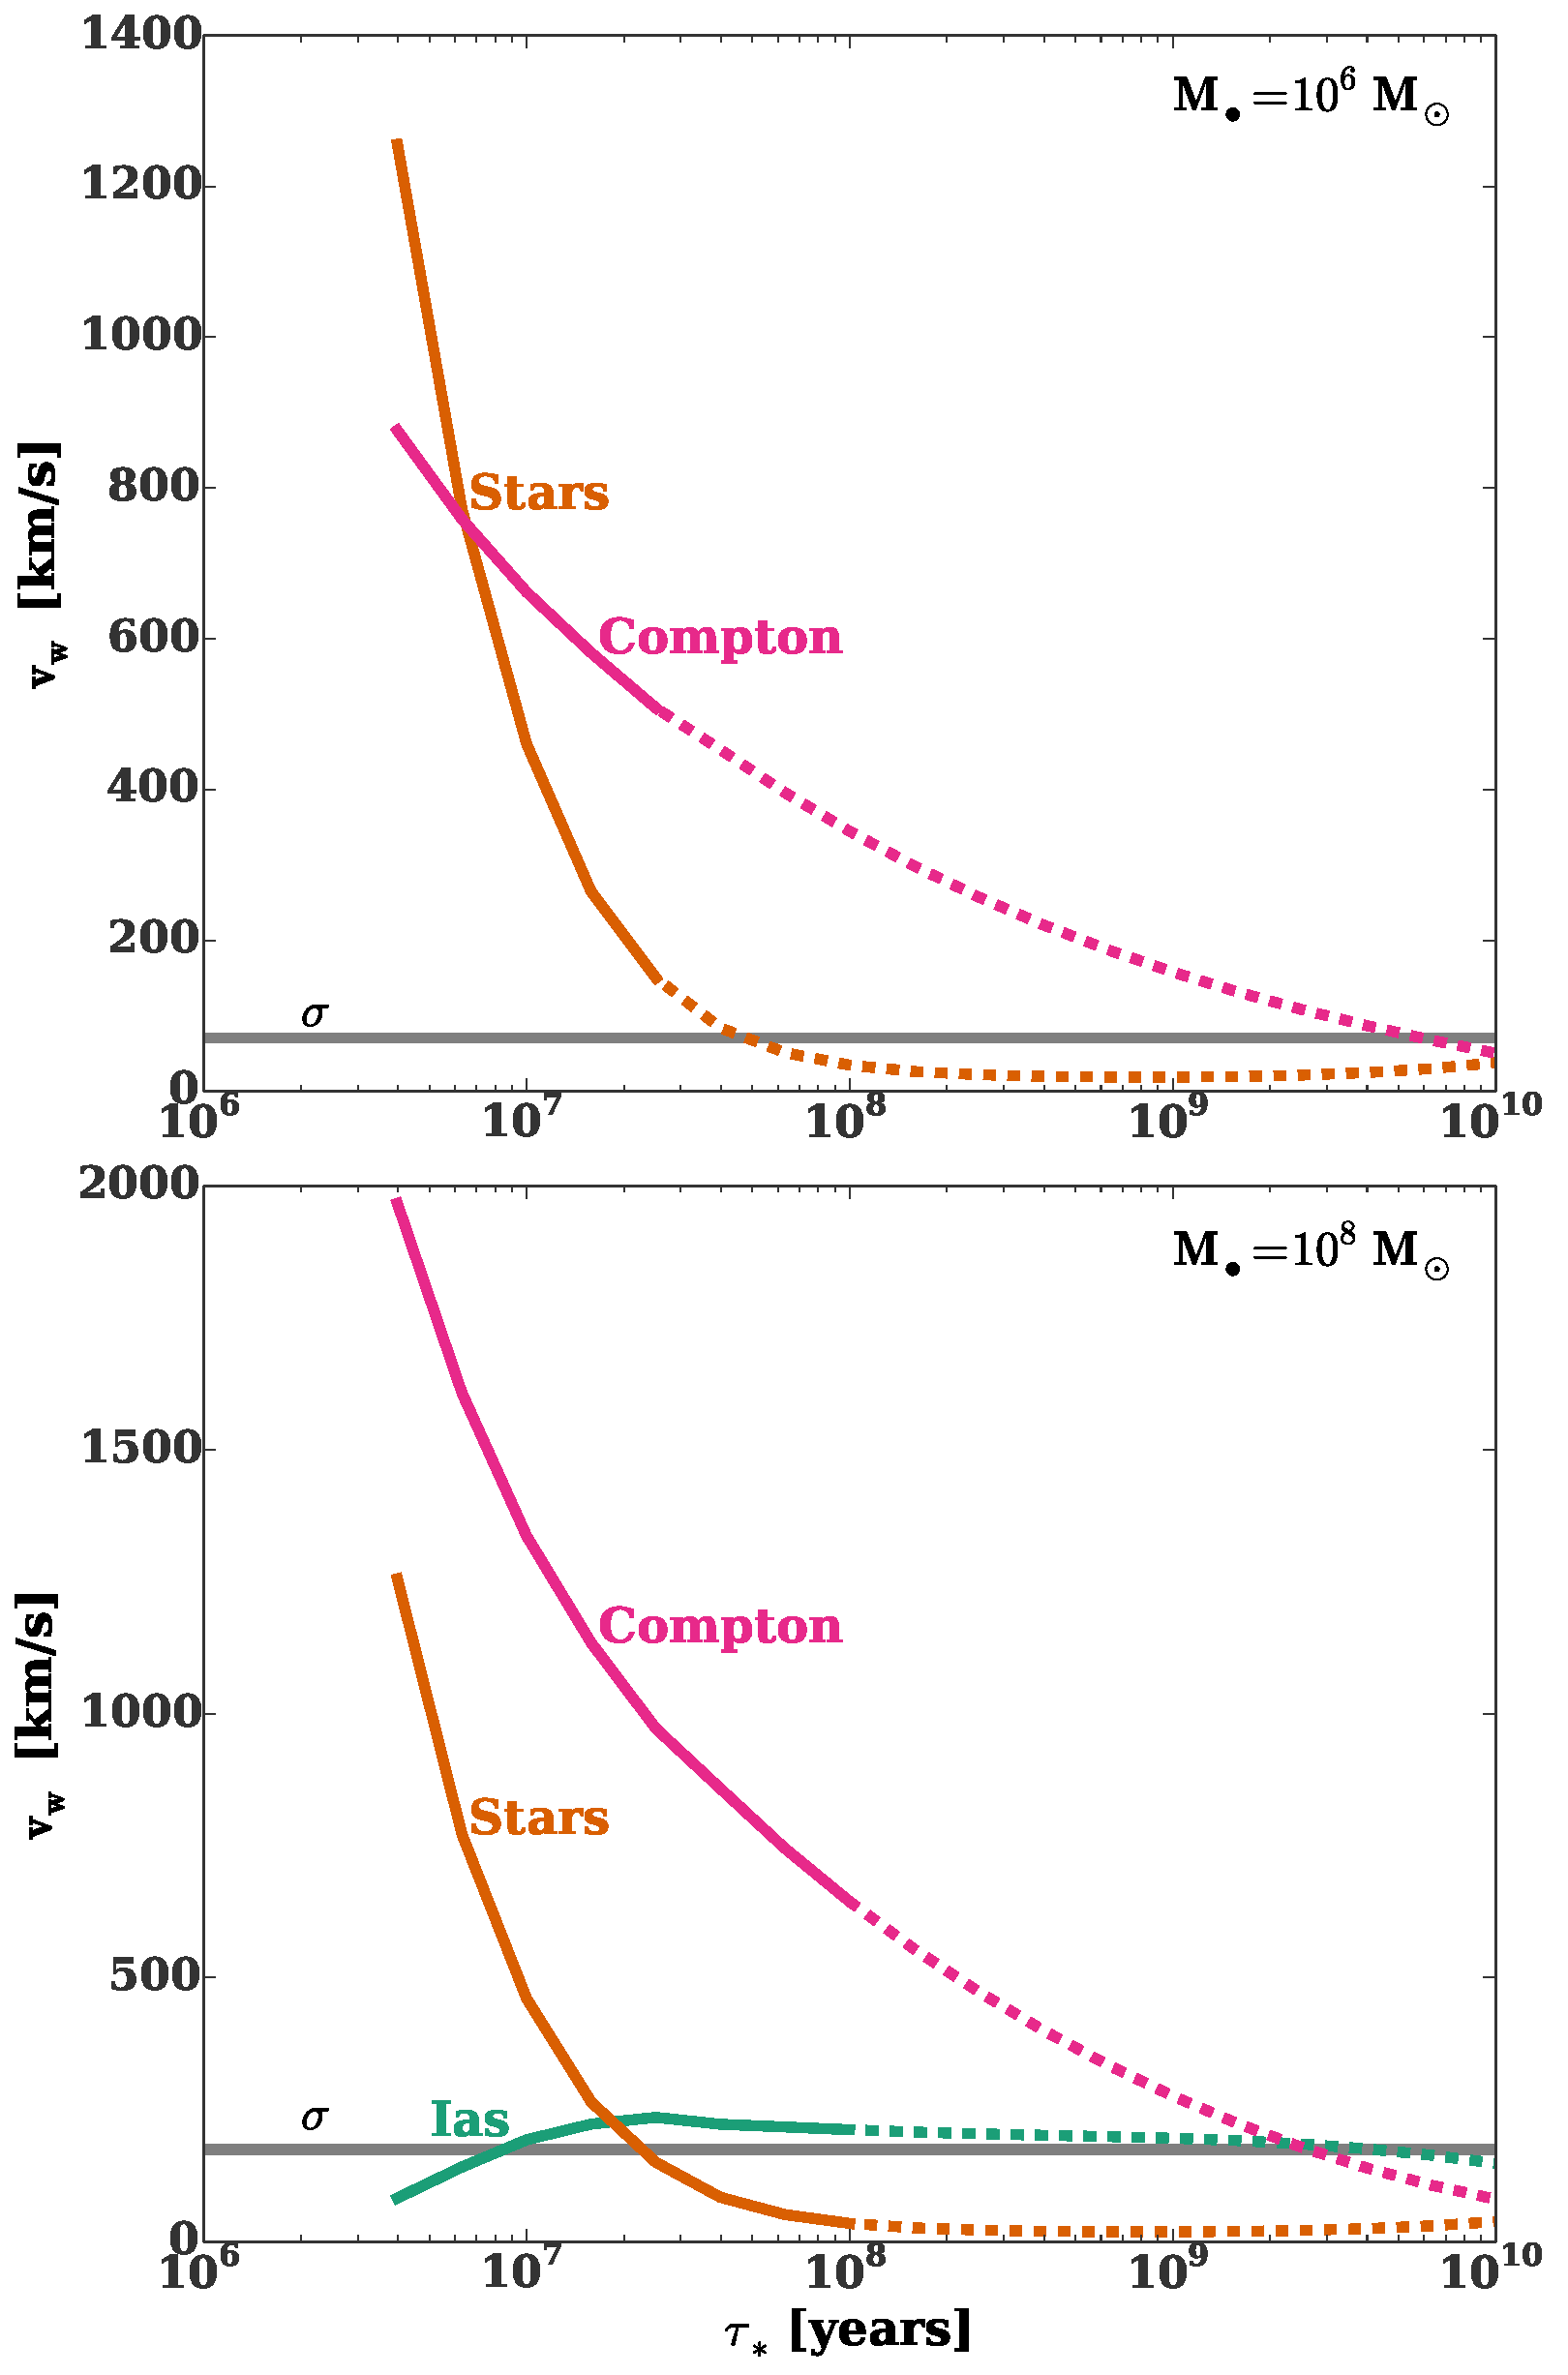
\includegraphics[width=\columnwidth]{vwSourcesImp.pdf}
\caption{\label{fig:vwSourcesImp} Sources contributing to
  the gas heating rate at time $\tau_{\star}$ after
  a single burst of star formation.  Top and bottom panels show black hole masses of $\Mbh=10^6 \Msun$ and $\Mbh= 10^8 \Msun$
  (both cusps with $\Gamma=0.8$).  Solid and dashed lines show the ranges of
  $\tau_{\star}$ for which the accretion flow is thermally stable and
  unstable, respectively, according to the ratio of $\dot{q}_{\rm
    heat}/|\dot{q}_{\rm rad}|$ near the stagnation radius
  (eq.~[\ref{eq:cooling3}]).  Shown with horizontal gray lines
  are the stellar velocity dispersion for each SMBH mass, estimated as $\sigma_0=\sqrt{3} \sigma_{\bullet}$ (eq.~[\ref{eq:Msigma}]).}
\end{figure}


\begin{figure}
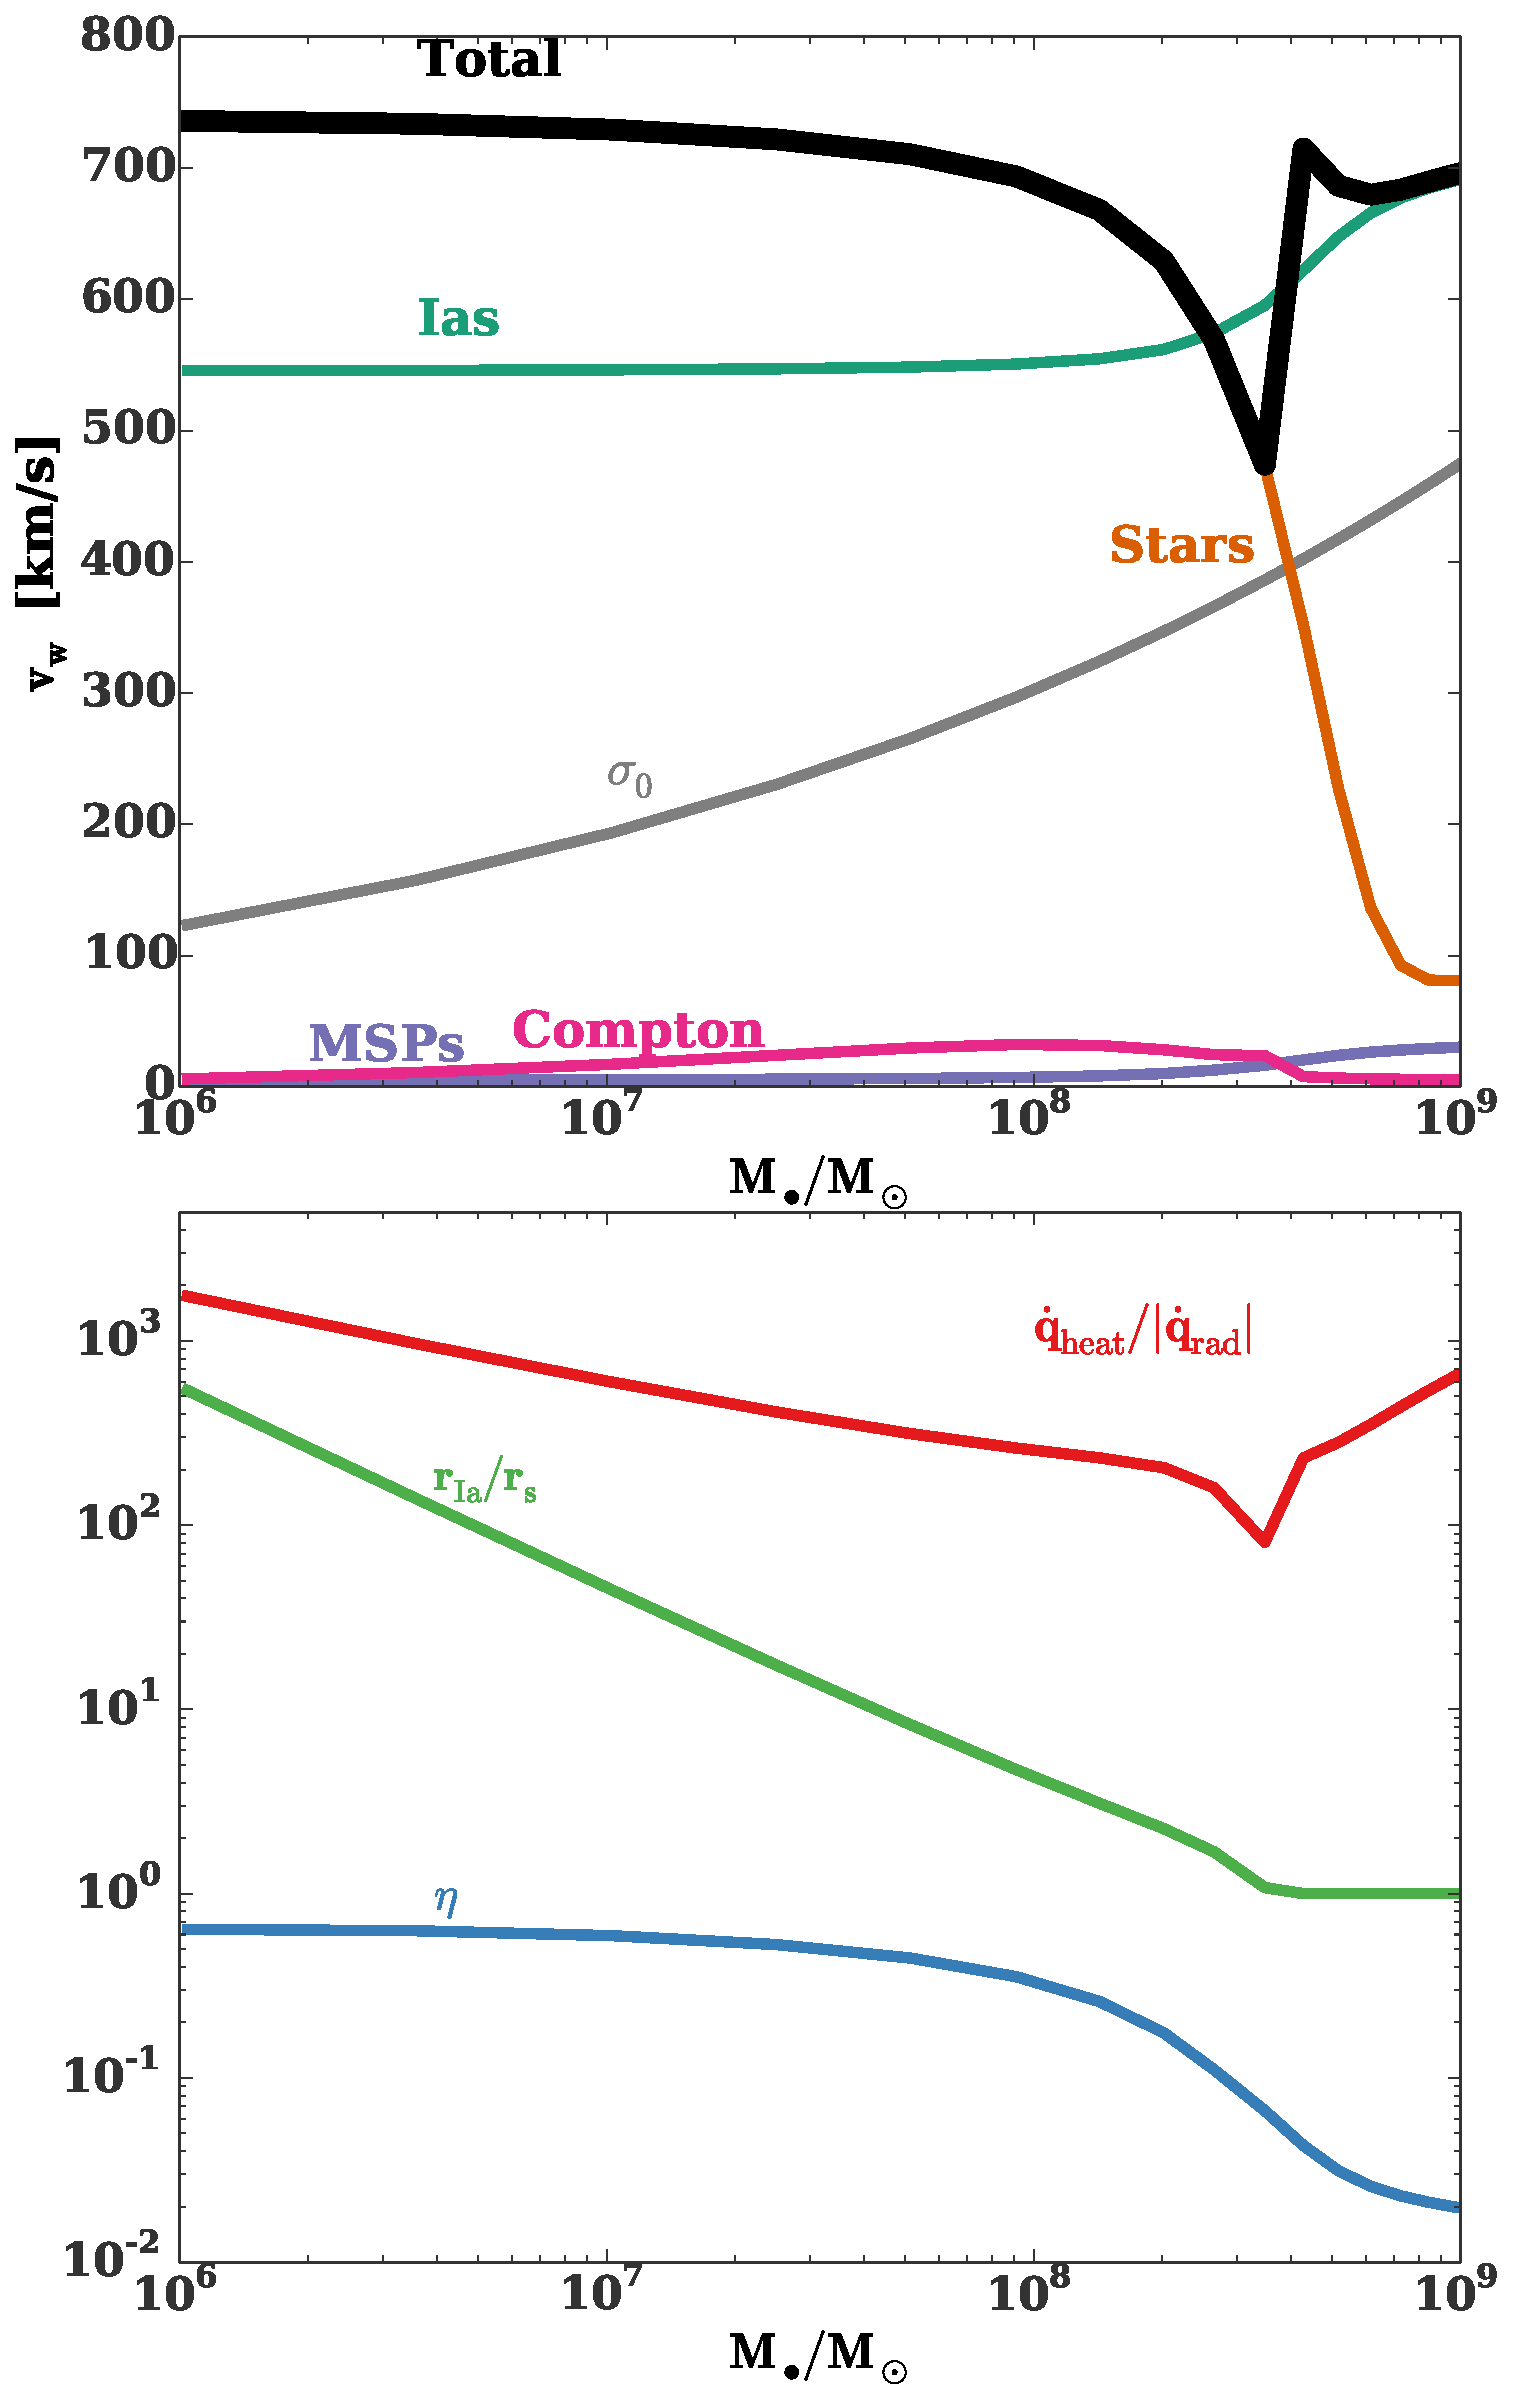
\includegraphics[width=\columnwidth]{vwSources.pdf}
\caption{\label{fig:vwSources} {\it Top Panel:} Sources contributing
  to the total heating rate of the CNM, $\vwO$ ({\it black}): stellar
  wind heating ({\it orange}), Ia supernovae ({\it green}),
  millisecond pulsars ({\it blue}), and compton heating ({\it pink}).
  Each heating source varies with black hole mass $\Mbh$ calculated
  for average SFHs from \citet{MosterNaab+:2013a}; see
  Appendix~\ref{app:windheat} for details.  {\it Bottom Panel:} The
  ratio of the total heating rate ($\dot{q}_{\rm heat} \propto
  v_{w}^{2}$) from the top panel to the radiative cooling rate
  ($|\dot{q}_{\rm rad}|$) at the stagnation radius (red), parameter
  $\eta$ characterizing stellar mass loss rate (eq.~[\ref{eq:q}]) as a
  function of black hole mass $\Mbh$, calculated for average star SFHs
  from \citealt{MosterNaab+:2013a} (blue), the ratio of Ia radius to
  stagnation radius as a function of $\Mbh$ (green), and the ratio of
  $\zeta/\zeta_{c}$ (purple), where $\zeta_c$
  (eq.~[\ref{eq:zetacrit}]) is the critical heating parameter $\zeta
  \equiv \sqrt{1+(v_w/\sigma_0)^2}$ below which outflows are
  impossible.  The latter quantity is evalulated using mean scaling
  relations for $r_b$, $\rinf$, and $\Gamma$ from the
  \citet{LauerFaber+:2007a} galaxy sample.}

 % $\Gamma=0.3
 %  \Mbheight^{-0.24}$, $\rinf=14 \Mbheight^{0.6}$ pc
 %  (eq~\eqref{\eqref{eq:rsoi}}), $\rb\simeq 106 \Mbheight^{0.39} $ pc
 %  (for $\Gamma<0.3$), and $\rb\simeq 100$ pc (for $\Gamma\geq 0.3$)
 %  {\bf Added zeta/zeta_c line but unfortunately caption became
 %    somewhat verbose (I don't think all of this description is
 %    necessary--maybe just say we use scaling relations based on Lauer
 %    et al. sample?) Also being so close to zeta/zeta_c=1 implies
 %    there is a limit to how much scatter we could explain just by
 %    variations in the heating rate}.

\end{figure}



\subsection{Combined Heating Rate} 
\label{sec:combined}


The total external gas heating rate, 
\begin{equation}
\vwO = \sqrt{(v_{w}^{\star})^{2} + (v_{w}^{\rm MSP})^{2} + (v_{w}^{\rm Ia})^{2} + (v_{w}^{\bullet})^{2}},
\label{eq:vtot}
\end{equation}
includes contributions from stellar winds, supernovae, pulsars, and
radiative SMBH feedback.  The strength of each heating source depends
explicitly on the SMBH mass and the stellar population in the galactic
nuclear region.  The latter could best be
described by a single star burst formation in the past, or by a more
continuous SFH that itself varies systematically
with the galaxy mass and hence $\Mbh$.

\subsubsection{Single Starburst}

Figure~\ref{fig:vwSourcesImp} shows the contributions of heating
sources as a function of time $\tau_{\star}$ after a burst of star
formation for black holes of mass $\Mbh = 10^{6} \Msun$ (top) and
$\Mbh = 10^{8} \Msun$ (bottom). The heating and mass input parameters
due to stellar winds, $v_{w}^{\star}(\tau_{\star})$ and
$\eta(\tau_{\star})$, are calculated as described in
Appendix~\ref{app:windheat} (Fig.~\ref{fig:vwImp}).  The SN Ia and
Compton heating rates, $v_{w}^{\rm Ia}$ and $v_{\rm w}^{\rm C}$, are
calculated from equations~\eqref{eq:vIa} and~\eqref{eq:vC},
respectively, which also make use of $\eta(\tau_{\star})$ as set by
stellar winds.\footnote{Both $v_{\rm w}^{\rm C}$ and $v_{\rm w}^{\rm
    Ia}$ (through $r_{\rm s}/r_{\rm Ia}$) depend on the total heating
  rate (eq.~[\ref{eq:vtot}]), requiring us to simultaneously solve a
  series of implicit equations to determine each.}  SN Ia heating
depends also on a convolution of the DTD (eq. [\ref{eq:DTD}]) and the
SFH, which reduces to the DTD itself for a single star burst.  We
account for the expected suppression of SN Ia heating resulting from
its non-steady nature by setting $v_{w}^{\rm Ia} = 0$ when the
stagnation radius (calculated {\it excluding} Ia heating) exceeds the
Ia radius $r_{\rm Ia}$ (eq.~[\ref{eq:rIa}]).  Heating from

Figure \ref{fig:vwSourcesImp} shows that stellar winds are the most
important heating source at early times, $\tau_{\star} \lesssim
10^{7}$ years.  Compton heating becomes more important at later times
due to (1) the higher accretion rates that accompany the overall
decrease in all sources of heating, coupled with (2) the persistently
high mass loss rates and gas densities associated with the still
relatively young stellar population.  Interestingly, for $M_{\bullet}
= 10^{6}M_{\odot}$, SN Ia dominate the heating briefly around 10$^{9}$
yr due to a window of time in which $r_{\rm Ia} < \rs$.  For high-mass
black holes (Fig.~\ref{fig:vwSourcesImp}, bottom panel), SN Ia
dominate at all times after $10^{7}$ yr.

As the total heating rate declines with time, the flow inevitably becomes thermally unstable according to the criterion $(\dot{q}_{\rm heat}/|\dot{q}_{\rm rad}|)_{r_{s}} \lesssim 10$
(eq.~[\ref{eq:cooling3}]), as shown by dashed lines in
Fig.~\ref{fig:vwSourcesImp}.  Compton heating is neglected in
calculating thermal stability because$-$unlike local stellar feedback
mechanisms$-$it is not clear that SMBH feedback is capable of stabilizing the
flow given its inability to respond instantaneously to local changes
in gas properties.  Thermally unstable flow is present throughout the single starburst case except at very early times, $\tau_{\star} \lesssim 10^7$ yr and at late times $\tau_{\star}
\gtrsim 10^{9}$ yr in the high $M_{\bullet}$ case.

Finally, note that MSP heating is negligibly small for fiducial parameters and hence
is not shown, while kinetic feedback is neglected given its uncertain efficiency ($\S\ref{sec:kinetic}$).

\subsubsection{Continuous SFH}
A single burst of star formation does not describe the typical star
formation history of most galaxies.  Qualitatively, smaller galaxies
will on average experience more recent star formation, resulting in
energetic young stellar winds and supernovae which dominate the gas
heating budget.  Massive galaxies, on the other hand, will on average
possess older stellar populations, with their heating rates dominated
by SN Ia (on large radial scales) and SMBH feedback.  We estimate the
average value of $\vwO$ as a function of SMBH mass for each heating
source by calculating its value using the average cosmic star
formation histories of \citet{MosterNaab+:2013a}.  Appendix
\ref{app:windheat} describes how the average SFH is
used to determine the stellar wind heating $v_{\rm w}^{\star}$ and
mass return parameter $\eta$ as a function of $M_{\bullet}$
(Fig.~\ref{fig:vwSources}; top panel).  SFHs are also
convolved with the Ia DTD distribution to determine the SN Ia heating.

Figure~\ref{fig:vwSources} shows $\vwO(M_{\bullet})$ from each heating
source (stars, MSPs, SNe Ia, and black hole feedback) calculated for
the average SFH of galaxies containing a given black hole mass.  The
younger stellar populations characterizing low mass galaxies with $\Mbh\lsim
3\times 10^{8} \Msun$ are dominated by stellar winds, with
$v_{w}^{\star} \gtrsim 700$ km s$^{-1}$.  Only for $\Mbh\gsim 3\times
10^{8} \Msun$ does the lack of young stellar populations significantly
reduce the role of stellar wind heating.  For these massive
galaxies, however, the Ia radius is sufficiently small that SN Ia contribute
a comparable level of heating, $v_{w}^{\rm Ia} \gtrsim 500$ km
s$^{-1}$ (SN Ia do not contribute to the heating in low mass galaxies because $r_{\rm Ia} > \rs$; bottom panel).  

Strikingly, we find that galactic nuclei that experience the same
average SFH as their host galaxies possess thermally stable flows
across all black hole masses.  An important caveat, however, is that
$\vw$ is generally only a few times higher than the stellar velocity
dispersion, i.e. $\zeta \sim \zeta_c$ (eq.~[\ref{eq:zetacrit}]).  This
implies that the true stagnation radius and SMBH accretion rate could
be larger than our analytic estimates, potentially resulting in
thermal instability in a significant fraction of galaxies.  The bottom
panel of Figure~\ref{fig:vwSources} also shows $\zeta/\zeta_c$, where
$\zeta_c$ is estimated from the best-fit power-law dependence of
$r_b$, $\rinf$, and $\Gamma$ on $M_{\bullet}$ from the
\citet{LauerFaber+:2007a} galaxy sample.  In other words, the CNM of a
significant fraction of massive ellipticals may be thermally unstable,
not necessarily because they are receiving lower stellar feedback than
the average for their galaxy mass, but due to the high heating
required for stability given the structure of their stellar potential.

Realistic variations (``burstiness") in the SFH
will also often produce lower stellar wind heating rates (Appendix
\ref{app:windheat}).  Figure \ref{fig:NickPlot2} shows the heating
rate as a function of average black hole mass for non-fiducial cases
in which the current ($z = 0$) star formation is suppressed by a
factor $\iota$ from its average $z = 0$ value, for a characteristic
timescale $\delta t_{\star}$.  For $\delta t_{\star} \lesssim 10^{7}$
yr, we see that $v_{\rm w}^{\star}$ is reduced by at most a factor of
$\approx 2$ from its average value, even for huge drops in the star
formation rate ($\iota \sim 10^{-3}$).  However, burstiness in the
SFH over longer timescales can suppress heating
more significantly.  When $\delta t_{\star} \gtrsim 10^8~{\rm yr}$,
$v_{\rm w}^\star$ becomes very sensitive to $\iota$: at $\iota=0.1$,
$v_{\rm w}^\star \approx 400~{\rm km~s}^{-1}$ in most galaxies, but
for smaller $\iota$, $v_{\rm w}^\star \approx 200~{\rm km~s}^{-1}$ (an
exception to this is in galactic nuclei with $M_\bullet \gtrsim
10^8~M_\odot$, where heating is stabilized by SN Ia).  Our use
of average cosmic SFHs is appropriate provided
local variations are either on short timescales ($\delta t_{\star}
\lesssim 10^7~{\rm yr}$), or limited in magnitude ($\iota \gtrsim
0.1$).  If both of these conditions are violated, then the effective
heating rates for all but the most massive galaxies (where Ia
explosions dominate) will fall by a factor $\gtrsim 4$ from our
fiducial volumetric averages, calculated using SFHs from \citet{MosterNaab+:2013a}.


\section{Implications and Discussion}
\label{sec:discussion}

\subsection{Black Hole Accretion Rates}
\label{sec:mdot}



\begin{figure}
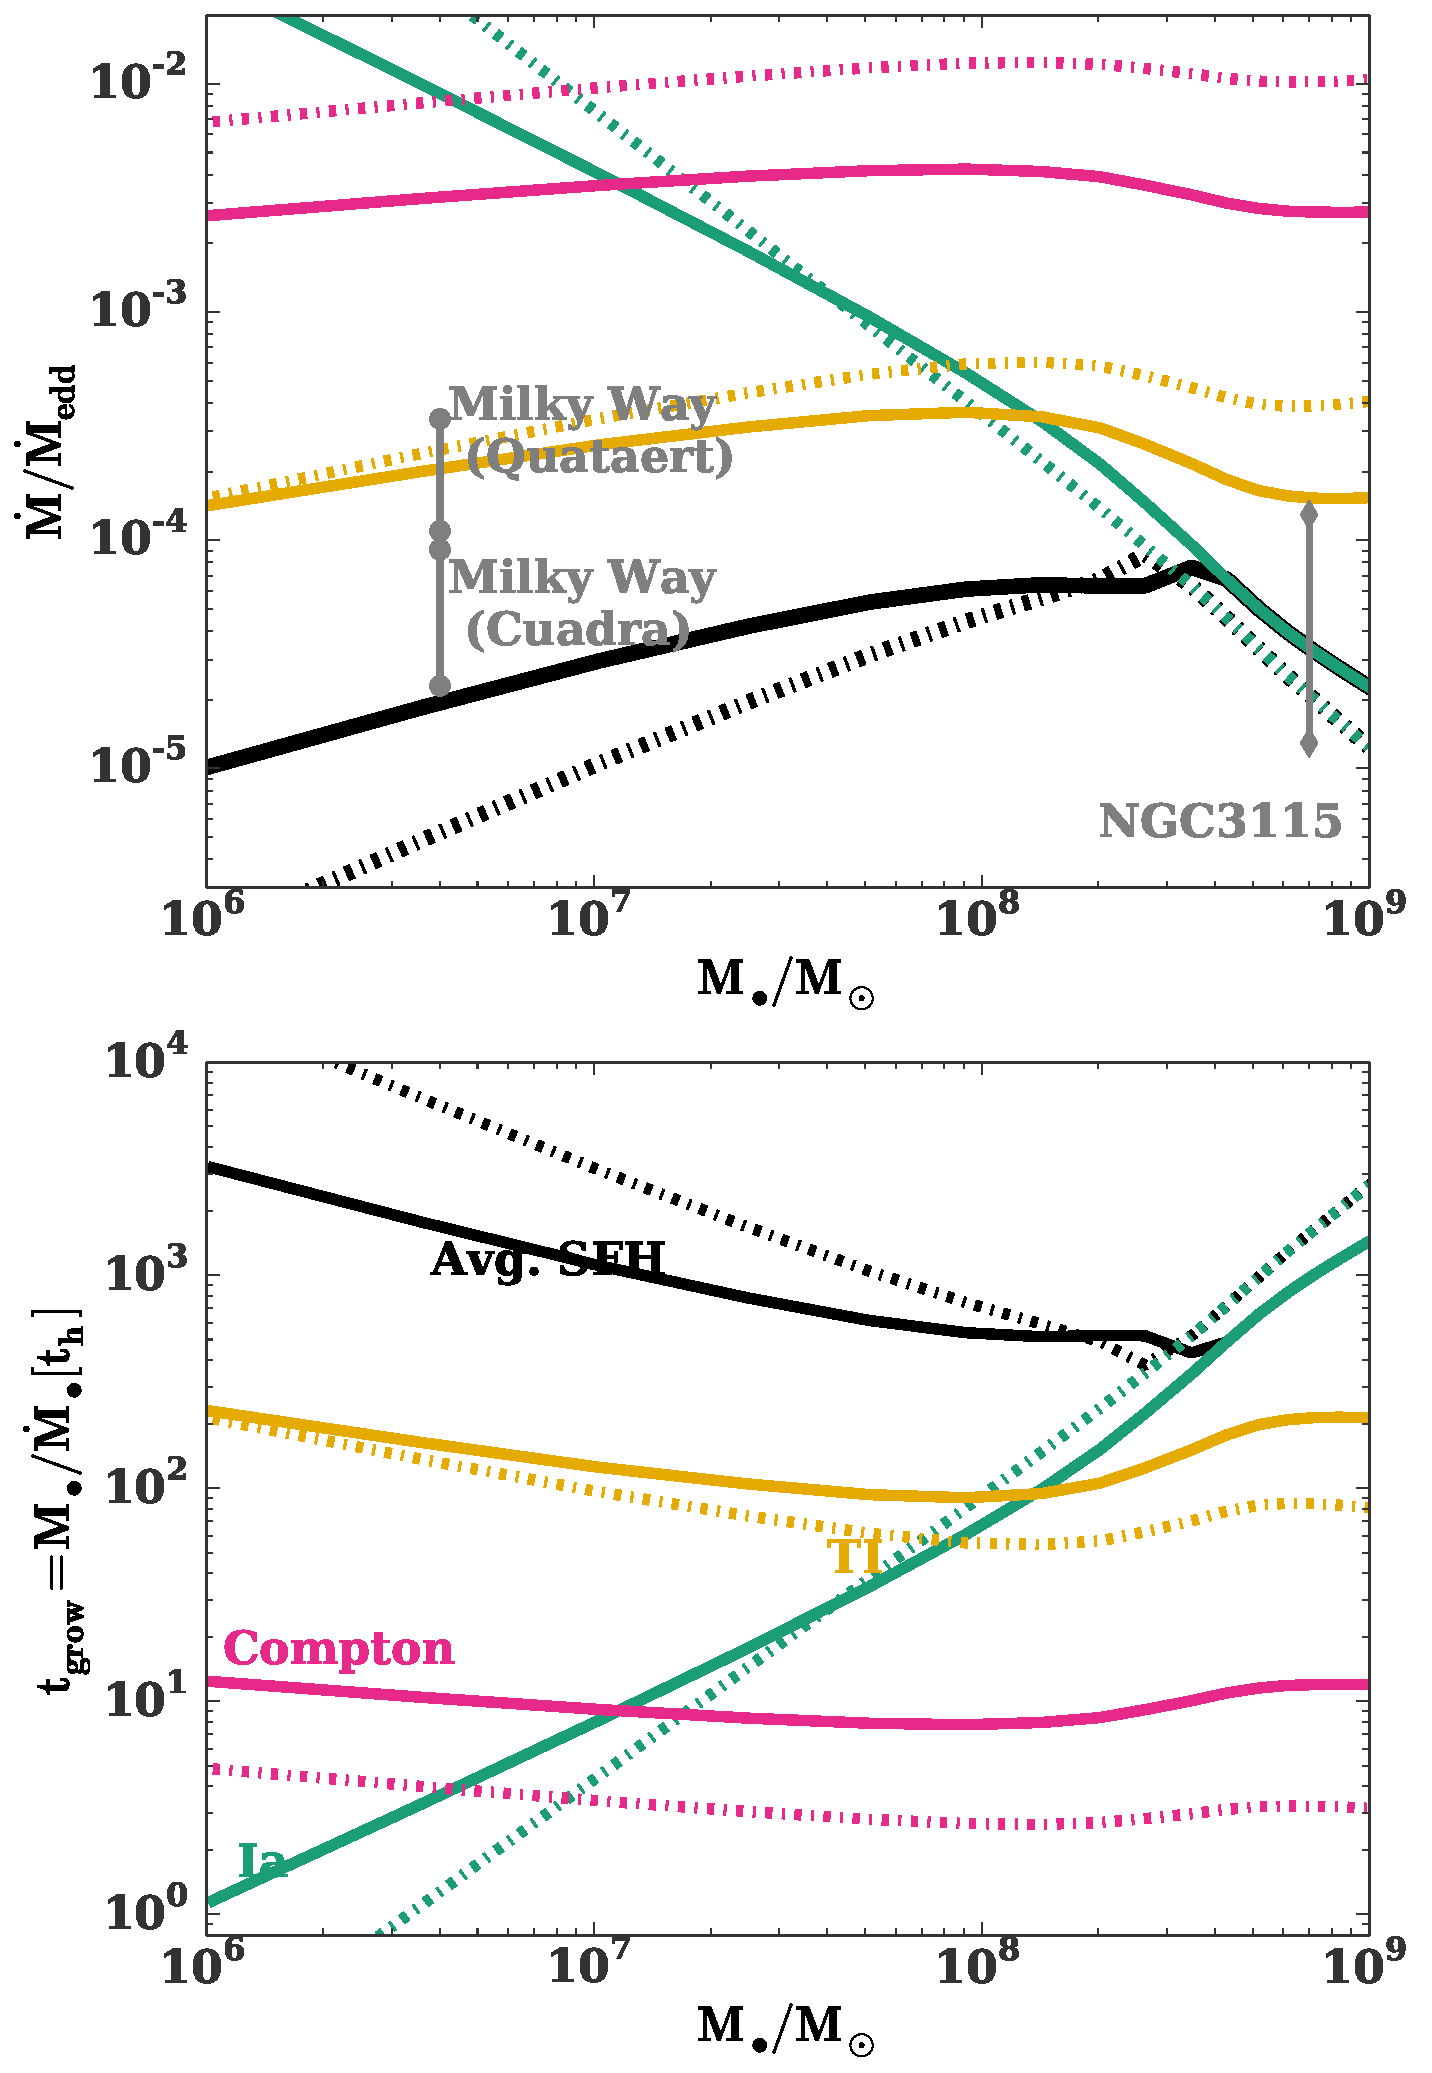
\includegraphics[width=\columnwidth]{mdot_sfr.pdf}
\caption{\label{fig:bh_growth} {\it Top panel:} Gas inflow rate
  $\dot{M}/\dot{M}_{\rm edd}$ as a function of black hole mass
  $M_{\bullet}$, shown for core ($\Gamma=0.1$, dot-dashed) and cusp
  galaxies ($\Gamma=0.8$, solid).  Black lines show the accretion rate
  calculated from equation (\ref{eq:eddr_analytic}) using the heating
  rate provided at $z = 0$ by the average star formation histories for
  each galaxy mass (Fig.~\ref{fig:vwSources}).  Teal lines show the
  maximum accretion set by Ia supernovae blow-out, $\dot{M}_{\rm Ia}$
  (\ref{eq:eddr_Ia}).  Red lines show the accretion rate obtained if
  Compton heating acts alone, $\dot{M}_{\rm C}$
  (eq.~[\ref{eq:MdotC}]).  Yellow lines show the maximum accretion
  rate for a thermally stable flow near the stagnation radius,
  $\dot{M}_{\rm TI}$ (eq.~[\ref{eq:Mdotmax}]).  Also shown are the
  inferred accretion rates of SgrA* from \citet{Quataert:2004a} (gray
  circles), for NGC3115 from \citet{ShcherbakovWong+:2014a} (gray
  diamonds), and for Swift J1644+57 from \citet{BergerZauderer+:2012a}
  (gray triangles).  {\it Bottom panel:} Growth times $t_{\rm grow}
  \equiv \Mbh/\dot{M}_{\bullet}$ in units of the Hubble time $\th$ for
  each of the accretion rates shown in the top panel, where
  $\dot{M}_{\bullet} = \alpha\dot{M}$, where $\alpha = 0.1$, to
  account for the fraction of inflowing mass lost to disk outflows on
  small scales.}
\end{figure}

Figure \ref{fig:vwSources} shows that the heating associated with the
average SFH of a galaxy is approximately constant
with SMBH mass, except for the largest black holes with $M_{\bullet}
\gtrsim 5\times 10^{8}M_{\odot}$.  For a fixed wind heating parameter,
the Eddington ratio $\dot{M}/\dot{M}_{\rm edd}$ increases $\propto
M_{\bullet}^{0.5(0.8)}$ for core(cusp) galaxies, respectively
(Fig.~\ref{fig:mdot_mass}; eq.~[\ref{eq:eddr_analytic}]).

Figure \ref{fig:bh_growth} (top panel) shows with solid lines the
accretion rate as a function of black hole mass for the average star
formation heating, calculated from equation (\ref{eq:eddr_analytic})
using our results for the total wind heating
(Fig.~\ref{fig:mdot_mass}).  This average accretion rate increases
from $\dot{M} \sim 10^{-6}-10^{-5}M_{\odot}$ yr$^{-1}$ for low-mass
black holes ($M_{\bullet} \sim 10^{6}M_{\odot}$) to $\dot{M} \sim
10^{-4}M_{\odot}$ yr$^{-1}$ for $M_{\bullet} \sim 10^{8}M_{\sun}$.
These fall below the maximum thermally stable accretion rate,
$\dot{M}_{\rm TI}$ (yellow lines), although in practice high mass core
galaxies may be thermally unstable as we do not include the
$\zeta<\zeta_c$ criterion in Fig.~\ref{fig:mdot_mass} (see
equation~\eqref{eq:cooling4}).
% , although they become closer at the highest
% black hole masses $\sim 10^{9}M_{\odot}$. 


For low mass black holes, blow out from SN Ia radius caps the SMBH
accretion rate at a value $\dot{M}_{\rm Ia} \sim
10^{-6}-10^{-5}M_{\odot}$ yr$^{-1}$ (green lines;
eq.~[\ref{eq:eddr_Ia}]), which is however not low enough to prevent
otherwise thermally-unstable flow at smaller radii.  For higher
$M_{\bullet}$ the stagnation resides close to the Ia radius so Ia
heating contributes to the steady gas heating rate, even if the energy
released by a single Ia is insufficient to unbind gas from the stellar
bulge (eq.~[\ref{eq:blowout}]).  This explains why the black and yellow lines mean at high $M_{\bullet}$.

Shown also for comparison in Figure \ref{fig:bh_growth} (top panel) is
the accretion rate onto SgrA* calculated by \citet{Quataert:2004a}.
Also show is the range of $\dot{M}$ for the low-luminosity AGN NGC3115
derived through detailed modeling by \citet{ShcherbakovWong+:2014a},
who find a range of accretion rates depending on the assumed model for
thermal conductivity\footnote{We expect this range would be have been
  smaller had \citet{ShcherbakovWong+:2014a} included saturation of
  the conductive flux.}.  The SgrA* rate exceeds our estimate of
$\dot{M}$ due to the average SFH for the same $M_{\bullet}$ by almost
two orders of magnitude.  This discrepancy can in part be understood
by the fact that star formation in the central parsec of the Milky Way
cannot be described as steady-state: feedback is instead dominated by
the stellar winds from the ring of young massive stars of mass $\sim
10^{4}M_{\odot}$ and estimated age $\sim 10$ Myr (e.g.,
\citealt{Schodel+07}).  Such a star formation history is better
described by our impulsive (starburst) scenario, for which the value
of $\eta \sim 100$ at $\tau_{\star} = 10^{7}$ yr
(Fig.~\ref{fig:vwImp}) is a factor of $\sim 100$ times higher than the
value of $\eta \sim 1$ predicted in the average SFH case
(Fig.~\ref{fig:vwSources}, bottom panel).


\subsection{Nuclear X-ray Luminosities}
\label{sec:Lx}

The unresolved core X-ray luminosities of nearby galactic nuclei
provide a powerful diagnostic of the SMBH accretion rates and how they
vary with SMBH mass and other galaxy properties (e.g., \citealt{Ho08}
and references therein).  Figure~\ref{fig:miller} shows our
predictions for $\langle L_{X} \rangle =\epsilon_X \dot{M} c^2$ as a
function of black hole mass, where $\epsilon_{X} = \alpha\epsilon_{\rm
  rad}\epsilon_{\rm bol}$, $\alpha = 0.1$ accounts for the fraction of
the inflowing matter loss to outflows from the accretion disk,
$\epsilon_{\rm rad}$ is the radiative efficiency of the accreted
matter, and $\epsilon_{\rm bol} = 0.1$ is the assumed bolometric
correction into the measured X-ray band for low luminosity AGN
(\citealt{Ho08}).  In all cases the value of $\langle L_X \rangle$ is
calculated using the average accretion rate for galaxies with core
($\Gamma = 0.1$) and cusp ($\Gamma = 0.8$) stellar density profiles,
using the mean power-law relationship $\Gamma = 0.3
\Mbheight^{-0.24}$, based on fitting the \citet{LauerFaber+:2007a}
galaxy sample.

The left panel of Figure \ref{fig:miller} is calculated assuming a
constant low value for the radiative efficiency of $\epsilon_X =
10^{-4}$, typical of those estimated for low luminosity AGN (e.g.,
\citealt{Ho:2009a}).  The right panel luminosities are calculated
instead assuming an efficiency of $\epsilon_X= \epsilon_{\rm
  bol}\epsilon_{\rm rad}$ that depends on the Eddington ratio as
predicted by MHD sheaing box simulations by \citet{Sharma+2007} (see
eq.~[\ref{eq:efficiency}] and surrounding discussion).  Shown for
comparison are the X-ray measurements (black stars) and upper limits
(gray triangles) from the sample of early-type galaxies compiled by
\citet{Miller+15} (cf.~\citealt{Gallo+10}).  A black line shows the
best power-law fit to the X-ray luminosity from \citet{Miller+15},
given by $\langle L_X/L_{\rm edd}\rangle \sim \Mbh^\alpha$ with
$\alpha = -0.2$ (see also \citealt{Zhang+09, Pellegrini10, Gallo+10}).
Also shown are the maximum accretion rates, respectively, for
thermally stable accretion (eq.~[\ref{eq:Mdotmax}]; yellow), as set by
SN Ia blow-out (eq.~[\ref{eq:eddr_Ia}]; teal), and as allowed by
Compton heating feedback (eq.~[\ref{eq:MdotC}]; pink).



\begin{figure*}
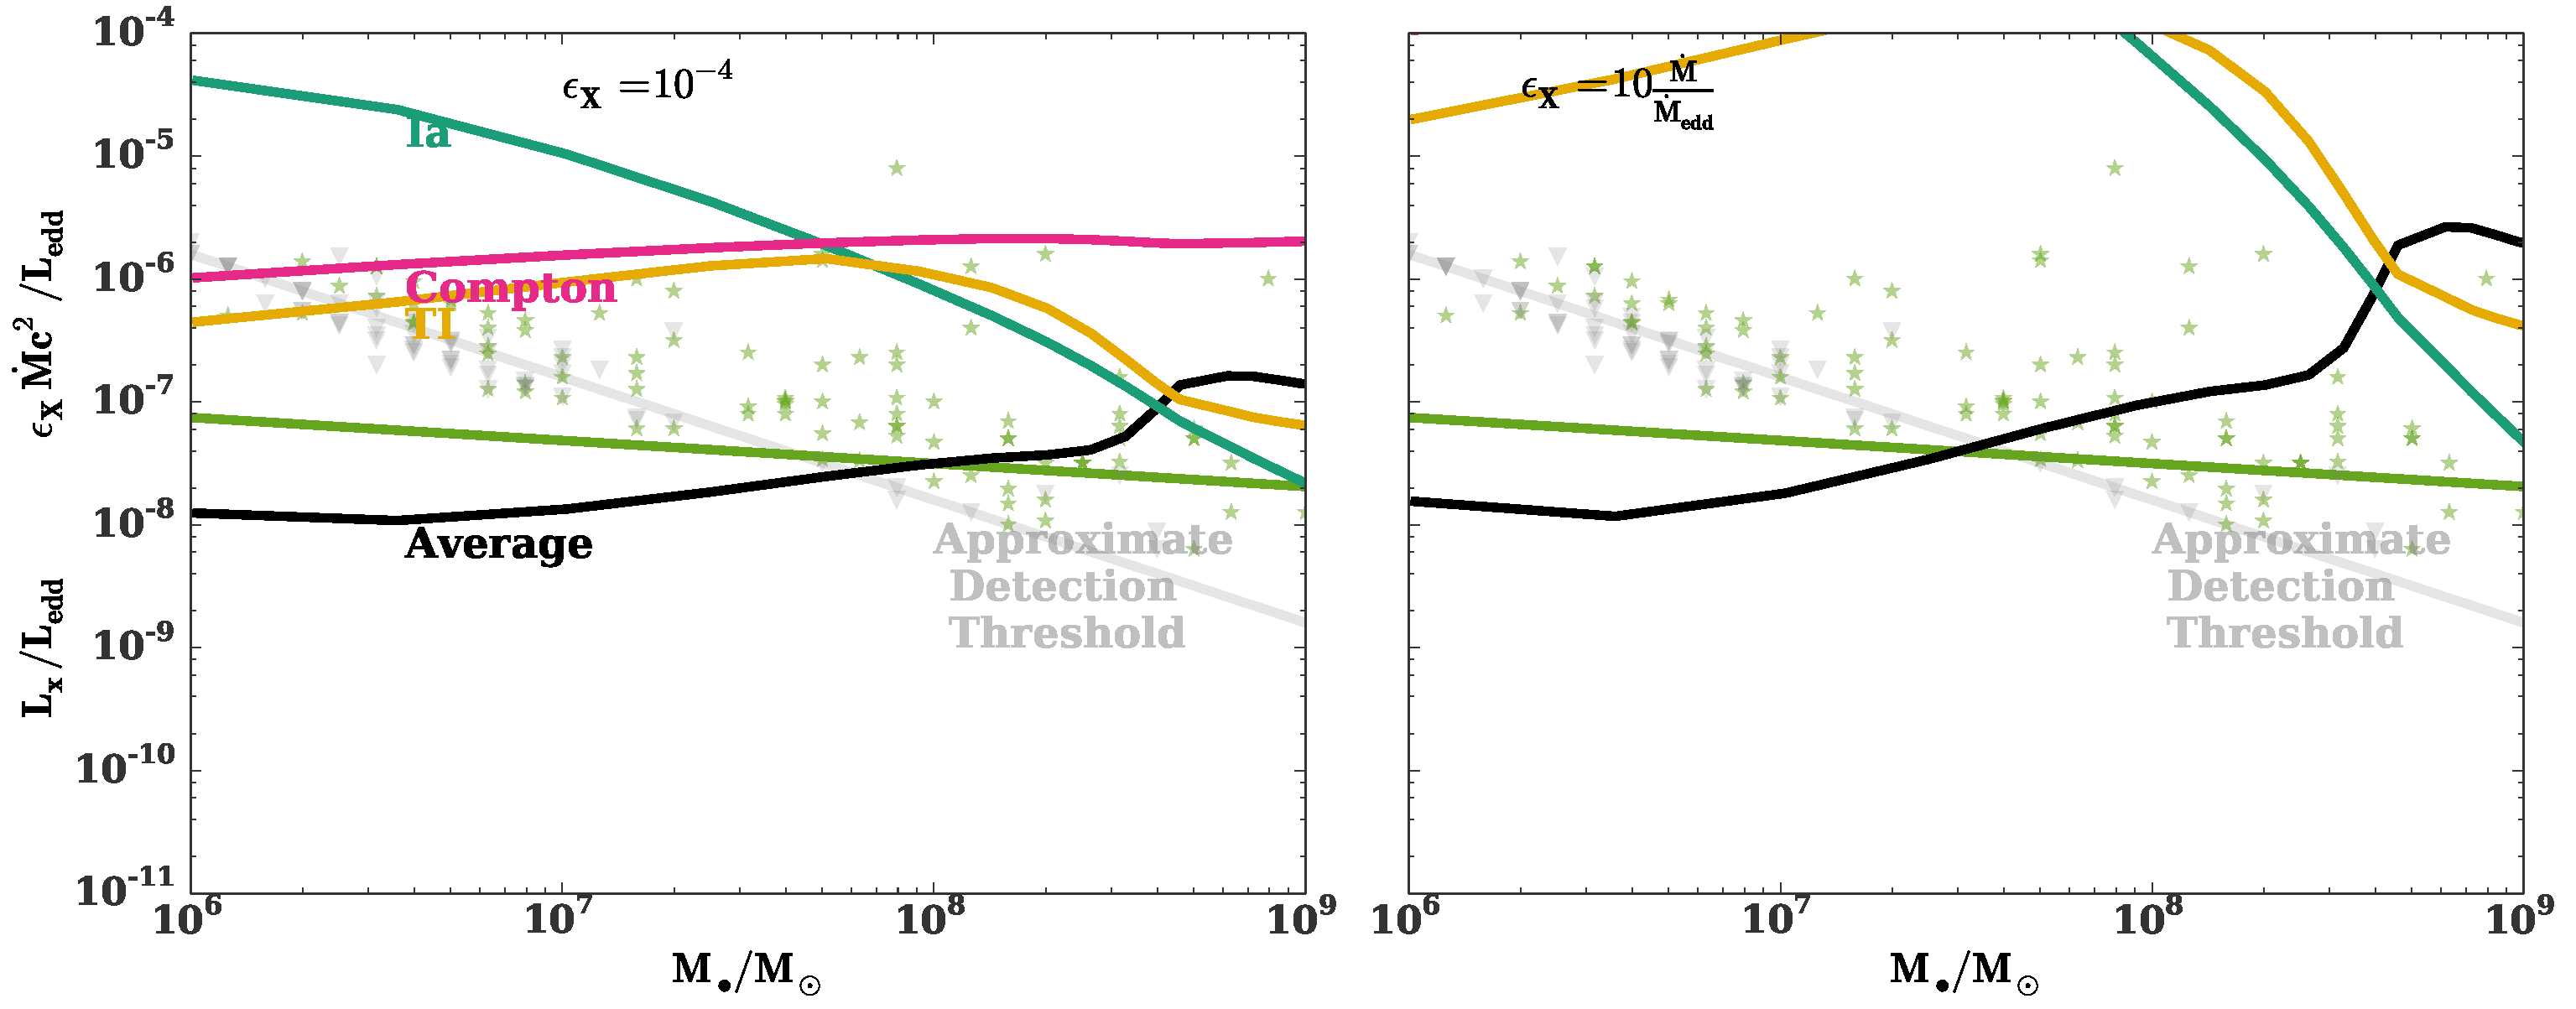
\includegraphics[width=\textwidth]{miller.pdf}
\caption{\label{fig:miller} Average nuclear X-ray luminosity, $\langle
  L_X \rangle = \epsilon_X \Mdot c^2$, as a function of SMBH mass.
  Green lines show our prediction in the case of heating due to the
  average SFH for galaxies corresponding to each black hole mass
  (Fig.~\ref{fig:bh_growth}), calculated using a power-law fit for the
  relationship $\Gamma(M_{\bullet})=0.3 \Mbheight^{-0.24}$ derived
  from the \citet{LauerFaber+:2007a} sample.  Shown for comparison are
  the measurements ({\it black stars}) and upper limits ({\it gray
    triangles}) for $L_X/L_{\rm edd}$ values, from the
  \citet{Miller+15} sample of early-type galaxies (a black line shows
  the best power-law fit $\langle L_X/L_{\rm edd}\rangle \propto
  M_{\bullet}^{\alpha}$, with $\alpha = -0.2$).  The left panel is
  calculated assuming a constant radiative efficiency
  $\epsilon_X=10^{-4} (\epsilon_{\rm bol}/0.1)$, while the right hand
  panel assumes $\epsilon_X= \alpha \epsilon_{\rm bol}\epsilon_{\rm
    rad}$, where $\epsilon_{\rm rad}$ is the radiative efficiency of
  low luminosity accretion disks calculated by \citet{Sharma+2007}
  (eq.~[\ref{eq:efficiency}]) and $\alpha = 0.1$ is the fraction of
  the mass inflowing on large scales that reaches the SMBH.  Shown for
  comparison are the X-ray luminosities calculated for the maximum
  thermally-stable accretion rate ({\it dashed orange line};
  eq.~[\ref{eq:Mdotmax}]); the SN Ia-regulated accretion rate ({\it
    dashed teal line}; eq.~[\ref{eq:eddr_Ia}]), and the Compton
  heating-regulated accretion rate ({\it dashed pink line};
  eq.~[\ref{eq:MdotCa}]), again all calculated for the average SFH
  corresponding to each SMBH mass.}
\end{figure*}

If the nuclei of elliptical galaxies are heated as expected for the
average SFH of galaxies with similar mass, then to first order we
predict that $\langle L_{X}/L_{\rm edd}\rangle$ should be a weakly
increasing function of BH mass.  This result is in tension with the
observed down-sizing trend that the average Eddington ratio is seen to
decrease (albeit weakly) with $M_{\bullet}$, especially in the model where
$\epsilon_X$ increases with the Eddington ratio.
However, one must keep in mind the enormous uncertainty in calculating
the luminosity of the accretion flow close to the black hole in a
single waveband based on the feeding rate on larger scales.  Also, if disk
outflows indeed carry away most of the infalling mass before it reaches X-ray
producing radii (e.g.~\citealt{Blandford&Begelman99};
\citealt{Li+13}), then the angular momentum of the infalling gas might
also influence the X-ray luminosity indirectly through the inflow efficiency $\alpha$, in a way that could depend systematically on the stellar population and hence $M_{\bullet}$.  However, in general the efficiency with which inflowing matter reaches the SMBH (and hence X-ray luminosity) would naively be expected to {\it decrease} with decreasing $M_{\bullet}$ due to the increasing angular momentum of low mass galaxies, exacerbating the tension between our findings and the observed downsizing trend.

Perhaps a more readily addressable test is whether a steady-state
accretion picture developed in this work can account for the the large
scatter, typically of $2-3$ orders of magnitude, in $L_{X}/L_{\rm
  edd}$ at fixed $M_{\bullet}$.  Scatter could result from the strong sensitivity of the accretion rate to the stellar wind
velocity and mass loss parameter, $\dot{M}/\dot{M}_{\rm edd} \propto
v_{w}^{-3.8(-2.4)}$ for core(cusp) galaxies, respectively
(Fig.~\ref{fig:mdot_mass}; eq.~[\ref{eq:eddr_analytic}]).  When
combined with the significant dependence of $v_w$ on stochastic
intermittency in the star formation history (Appendix
\ref{fig:NickPlot2}), this can lead to order of magnitude differences
in $\dot{M}$.  However, we note that $v_w$ is not expected to vary by more than a factor of a few for a thermally-stable flow, limiting the allowed variation of  $\dot{M}/\dot{M}_{\rm edd}$.  Variations in $L_{X}/L_{\rm
  edd}$ could also result from differences in angular momentum of the infalling gas from galaxy to galaxy, resulting in differences in the fraction of the gas lost to outflows.  Also potentially contributing is the order of magnitude difference, at
fixed $v_w$ and $M_{\bullet}$, between $\dot{M}$ for core and cusp
galaxies (Fig.~\ref{fig:bh_growth}).  Differences in $\dot{M}$ are
augmented by the theoretical expectation that $L_{\rm X} \propto
\dot{M}^{2} $ for radiatively inefficient flows.




\subsection{Steady Accretion versus outbursts}
\label{sec:cycle}

It is also possible that many of the \citet{Miller+15} sample of
galactic nuclei are not accreting in steady state.  This is supported by the fact that many of the X-say luminosities in Figure \ref{fig:miller} lie above the predictions for stable accretion, i.e., $L_X \gtrsim \epsilon_X \dot{M}_{\rm TI}c^{2}$ (yellow line), at least for our choice of radiative efficiency.  

Within our steady state solutions gas outside the stagnation radius $\rs$ is being blown
out in wind. However, for very massive galaxies ($\Mbh\gsim 10^8
\Msun$) the energy injected into the gas is not enough to truly blow
the gas out of the potential well of the galaxy. This gas is likely to
build up on the outskirts of the galaxy until a thermal instability
develops, causing the CNM to undergo cyclic oscillations of rapid
cooling and high accretion rates, followed by quiescent periods once
gas has been consumed and/or AGN feedback becomes effective. Such
cycles are seen in numerical simulations of elliptical galaxies on
large scales and long timescales (\citealt{Ciotti+10}).  Evidence for
such periodic outbursts includes observations showing that a fraction
of early-type galaxies in the local universe have undergone recent ($<
1-2$ Gyr old) star formation episodes (\citealt{Donas+07}).

 
%Furthermore, our SFH-averaged accretion rates are derived using
%analytic expressions for the stagnation radius that may underpredict
%the true accretion rate if $\zeta < \zeta_c$, as may occur in massive
%core galaxies with large break radii.

If the actual radiative efficiency is lower than our fiducial
assumption, then an even larger fraction of the X-ray detections would lie above the
predictions for stable accretion.  For example, we assume that a fraction $\alpha = 0.1$ 
of the mass inflow rate reaches the SMBH, but this fraction could be considerably smaller. In such a case the X-ray detected galaxies will be experience less heating than we calculate for the average SFH, and may not be stably accreting at all.  This is plausible given that the \citet{Miller+15} sample includes only early-type galaxies with older stellar populations than the average for their stellar mass.

Figure \ref{fig:bh_growth} (top panel) also shows that $\dot{M}_{\rm
  C} > \dot{M}_{\rm TI}$ across all black hole masses.  This indicates that Compton heating is not sufficient to produce a thermally stable accretion rate, at least for conditions corresponding to the average SFH.


Similar cyclic AGN activity could occur on the smaller radial scale of
the sphere of influence (e.g.~\citealt{Yuan&Li11},
\citealt{Cuadra+15}).  In this case the large scatter in the X-ray
luminosities shown in Fig \ref{fig:miller} could result from the wide
range of inflow rates experienced over the course of a cyclic episode
between instabilities and periodic nuclear outbursts. 

If the galaxies with measured $L_{\rm X}$ at low $M_{\bullet}$
in Figure \ref{fig:miller} are indeed in a state of thermally-unstable
outburst, then some of the galaxies with X-ray upper limits could be contributing to a separate population of thermally-stable, steadily accreting nuclei.  Such a population could include SgrA*, which has a much lower X-ray luminosity for its SMBH mass than predicted by the \citet{Miller+15} trend.  A potentially bimodal population of steady and outbursting galactic nuclei calls into question the practice of using simple extrapolations of power-law fits to the $L_{\rm X}(M_{\bullet}$) relationship to low $M_{\bullet}$ to constrain the occupation fraction of SMBHs in the nuclei of low mass
galaxies.



\subsection{SMBH Growth Times }
\label{sec:growth}

Low-mass AGN in the local universe with $M_{\bullet} \lesssim 3\times
10^{7}M_{\odot}$ are observed to be growing on a timescale comparable
to the age of the universe, while the most massive SMBHs with
$M_{\bullet} \gtrsim 10^{9}M_{\odot}$ possess local growth times which
are more than 2 orders of magnitude longer (\citealt{Heckman+04};
\citealt{Kauffmann&Heckman09}).

The bottom panel of Figure~\ref{fig:bh_growth} shows the SMBH growth
time, $t_{\rm grow} \equiv M_{\bullet}/\dot{M}_{\bullet}$, for each accretion
rate shown in the top panel, where we remind that $\dot{M}_{\bullet} = \alpha\dot{M}$, where $\alpha = 0.1$.  For SMBHs which accrete steadily at the
rate set by the stellar wind heating due to the average star formation
history of their host galaxies, we see that $t_{\rm grow}$ exceeds the
Hubble time by 2$-$4 orders of magnitude across all $M_{\bullet}$.
Steady accretion therefore cannot explain the growth of low mass black
holes, a fact which is not surprising given that approximately half of
this growth occurs in AGN radiating within 10 per cent of their
Eddington rate (\citealt{Heckman+04}).  Such high accretion rates
likely instead require an source of gas external to the nuclear
region, triggered either by galaxy mergers associated with the
hierarchical growth of structure or thermal instabilities on larger,
galactic scales (e.g.~\citealt{Ciotti+10}, \citealt{Voit+15}).  
%In
%support of this, \citet{Kauffmann&Heckman09} find that the growth of
%low mass black holes is dominated by young stellar bulges which have a
%log normal distribution of Eddington ratios peaked at
%$\Mdot/\dot{M}_{\rm edd} \sim 0.01$. 

That the growth time associated with thermally-unstable accretion
(yellow line in Fig.~\ref{fig:bh_growth}) exceeds the Hubble time
across all SMBH masses highlights the fact that significant black hole
growth in the local universe cannot result from thermally-stable
steady accretion of gas lost from the surrounding stellar population
studied in this paper.  Gas blow-out by SN Ia cannot alone prevent the
growth of low-mass black holes, as indicated by the low growth times
$\ll t_{\rm h}$ allowed by Ia heating (green lines), although Ia
heating could play in principle a role in capping the growth rate of
$\gtrsim 10^{8}M_{\odot}$ black holes, again depending on the
efficiency of Ia heating and whether the galaxy is a core or cusp.


\subsection{TDE Jets}
\label{sec:TDE}

Our results also have implications for the environments encountered by
relativistic jets from TDEs.  For low-mass SMBHs with $M_{\bullet}
\lesssim 10^{7}M_{\odot}$, such as that responsible for powering the
transient {\it Swift} J1644+57 (\citealt{Bloom+11}), we predict gas
densities of a $n \sim 0.3-3$ cm$^{-3}$ on radial scales of 0.3 pc for
wind heating rates within the physically expected range $v_{\rm w}
\sim 500-1000$ km s$^{-1}$ (Fig.~\ref{fig:profiles}).  These values
are within the range estimated by modeling the radio afterglow of {\it
  Swift} J1644+57 (\citealt{Metzger+12},
\citealt{BergerZauderer+:2012a}), as shown in
Fig.~\ref{fig:bh_growth}.

\citet{BergerZauderer+:2012a} infer a flattening of the gas density
profile of the host of J1644+57 on radial scales $r \gtrsim 0.4$ pc
(their Fig.~6) which looks qualitatively similar to the shape density
profile we predict for core galaxies (Fig.~\ref{fig:profiles}, solid
line).  To obtain such a flattening on the inferred radial scales
would require a black hole of $\Mbh\sim 10^7 \Msun$.  However, this is
inconsistent with the break in the gas density seen at $\sim 0.6$ pc
by \citet{BergerZauderer+:2012a}, which should correspond to the break
radius of the {\it stellar density} profile, thus implying an
unrealistically small SMBH mass of $\Mbh\simeq 100\Msun$ according to
the mean $r_b-M_{\bullet}$ relationship \citep{LauerFaber+:2007a}.
Alternatively, the observed density break in J1644+57 could result
from the outer edge of a sub-parsec nuclear star cluster (e.g.,
\citealt{Carson+15}).  The high stellar densities of such a compact
star cluster could greatly enhance the TDE rate
(e.g.~\citealt{Stone&Metzger15}), possibly making this association
uncoincidental.  On the other hand, we note that some models for J1644+57  (e.g., \citealt{Tchekhovskoy+2014}) favor a much smaller black hole ($10^5-10^6 \Msun$) than we estimate would be required to produce the observed inner break.

% based on the observed jet power, the jet
%shut-off time (if linked with the accretion becoming sub-Eddington), and an
%observed QPO in the x-ray light curve favor a smaller black hole {\bf
 % AG Gone mad!}. 


\subsection{Regulation by SMBH Kinetic Feedback}
\label{sec:kinetic}

Our analysis of SMBH feedback has focused on Compton heating instead
of kinetic feedback, since the effects of radiative feedback are
relatively straightforward to calculate from the properties of the
accretion flow.  However, it is possible kinetic feedback from SMBH
outflows could play an equal or greater role in regulating accretion,
even in low luminosity AGN.

Our simple parameterization of kinetic feedback (eq.~[\ref{eq:vjet}])
assumes a uniform volumetric heating and predicts an effective wind
velocity which increases with SMBH mass as $v_{w}^{\bullet} \propto
M_{\bullet}^{0.33(0.28)}$ for core(cusp) galaxies, respectively.
Coupled with the dependence of the SMBH accretion rate on the wind
heating, $\dot{M}/\dot{M}_{\rm edd} \propto
M_{\bullet}^{0.76(0.48)}v_{w}^{-3.8(-2.4)}$ (Fig.~\ref{fig:mdot_mass};
eq.~[\ref{eq:eddr_analytic}]), a dominant source of kinetic feedback
of the form we have adopted leads to an Eddington ratio dependence on
SMBH mass of $\dot{M}/\dot{M}_{\rm edd} \propto
M_{\bullet}^{-0.5(-0.2)}$.

This prediction is also consistent with the observed dependence of
$\langle L_{X}/L_{\rm edd} \rangle$ in elliptical galaxies
(Fig.~\ref{fig:miller}, green line), suggesting that accretion
regulation by kinetic feedback could play a role in determining the
X-ray luminosities of elliptical galaxies.  However, our assumption
that kinetic outflows heat the gas uniformly in volume is rather
arbitrary and would need to more rigorously justified by numerical
studies of how jets or disk outflows couple energy to their gaseous
environment.  As already discussed, it is furthermore unclear whether
a steady-state accretion model is at all relevant in the case when
SMBH feedback dominates due to the time delay between the small scale
accretion flow and the thermodynamic response of the CNM on larger
scales.

%For a fixed $r_{\rm heat}$, the effective heating rate from kinetic outflows $v_{\rm w}^{\bullet} \propto r_{\rm s}^{1-\Gamma/2} \propto M_{\bullet}^{1-\Gamma/2}v_{w}^{\Gamma-2}$ is proportional to $v_{w}$
%to a negative power (where we have used of eq.~[\ref{eq:stag_simple}]).  Thus, as in the case of Compton heating, kinetic heating could in principle  `self-regulate' insofar as a lower heating rate results in a higher accretion rate, which in turn results in stronger jet feedback.  
%However, although both radiative and kinetic feed-back process seem capable of producing sufficient heating to offset radiative cooling and prevent instability (e.g., $v_w \gtrsim v_{\rm TI}$; eq.~[\ref{eq:cooling3}]), this is somewhat misleading because black hole feedback depends on the central accretion rate, which (unlike stellar feedback) does not respond instantaneously to changes in the thermodynamic properties of the gas on larger scale.  Thus, even if the AGN heating balances cooling on average, the flow may still experience limit cycle behavior in this case (\citealt{Yuan&Li11}).   


%\subsection{Jet Power Correlation}

%Accretion rates onto SMBHs can in principle be estimated directly by
% assuming Bondi accretion and using high resolution X-ray
% observations to estimate the gas temperature and density near the
% Bondi radius.  This technique has led to the intriguing conclusion
% that the Bondi accretion power correlates with the AGN jet power
% (e.g., \citealt{AllenDunn+:2006a}; \citealt{Russell+13};
% \citealt{FujitaKawakatu+:2014a}), the latter estimated from the
% energy required to inflate the observed cavities within the X-ray
% emitting gas.  In practice is it almost never possible to resolve
% the Bondi radius, therefore requiring all such studies to
% extrapolate the observed gas temperature and density profiles to
% smaller radial scales.

\section{Conclusions}
\label{sec:conclusions}

We have calculated steady-state models for the hot gaseous
circumnuclear media of quiescent galaxies, under the assumption that
gas is supplied exclusively by stellar wind mass loss and heated by
shocked stellar winds, supernovae and black hole feedback.  We compute
solutions for a range of different black hole masses, heating rates,
and observationally-motivated stellar density profiles.  Our numerical
results (Table \ref{table:models}) are used to verify and calibrate
analytic relationships (Appendix \ref{app:rs}, \ref{app:be}).  We use
the latter to explore systematically how the SMBH accretion rate
varies with black hole mass and the galaxy's SFH.  Our results for
$\dot{M}(\Mbh)$ are compared with observed trends of the nuclear X-ray
luminosities of quiescent SMBHs and low luminosity AGN.  Our conclusions are summarized as follows.

  \begin{enumerate}
  \item A stagnation radius, $\rs$, divides the nuclear gas between an
    accretion flow and an outgoing wind. In steady-state the gas inflow
    rate towards the black hole is proportional to the stellar mass
    enclosed inside of $\rs$.  In the limit of strong heating, the
    stagnation radius resides interior to the SMBH influence radius
    and coincides with the Bondi radius (eq.~[\ref{eq:rbondi}]), and
    the Bernoulli parameter of the flow at large radii is positive
    (Appendix \ref{app:be}).  In the limit of weak heating ($\zeta <
    \zeta_c$; eq.~[\ref{eq:zetacrit}]), the stagnation radius moves to
    large radii, near or exceeding the stellar break radius $r_b \gg
    r_{\rm inf}$, greatly increasing the density of gas on smaller
    radial scales.

  \item Including the effects of heat transport by electron conduction
    results in at most order unity changes to the key properties of
    the flow (e.g. stagnation radius, mass accretion rate, and thermal
    stability) for causal values of the conduction saturation
    parameter $\phi < 0.1$ (eq.~[\ref{eq:conduction}]).  Angular
    momentum is also unlikely to invalidate our spherically symmetric
    model on large scales, given observationally inferred rotation rates of galactic nuclei
    near the stagnation radius ($\S\ref{sec:rotation}$). 
%However, on
 %   small scales gas would encounter a centrifugal barrier which would
  %  cause much of the gas flowing inwards on large scales to be driven
   % outwards in an outflow (as in \citealt{Li+2013}). 

\item Radiative cooling has a more pronounced influence on the flow
  structure.  Cooling becomes important when the
  radiative cooling rate exceeds the gas heating rate near the
  stagnation radius, where the gas is in nearly hydrostatic equilibrium (Fig.~\ref{fig:TI}).  This condition is approximately equivalent to
  the $t_{\rm cool} \gg t_{\rm ff}$ criterion for thermal instability advocated by
  \citet{McCourt+12} and \citet{Li&Bryan14a}.  The transition in the flow properties that occurs as heating is reduced may represent a true ``thermal instability" (hot ISM condensing into a cooler clouds), or it may simply represent an abruption transition from a steady inflow-outflow solution to a global cooling flow.  We leave distinguishing between these possibilities to future work.  

\item The location of the stagnation radius, and hence the SMBH
  accretion rate, is a sensitive function of the gas heating rate
  $\propto v_w^{2}$.  Quantitatively, $\rs\propto v_w^{-2}$, implying
  that $\Mdot\propto v_w^{-3.8 (-2.4)}$ for fiducial core (cusp) galaxies.
  However, $\Mdot$ can increase even more rapidly with decreasing
  $v_w$ for two reasons: (1) when $v_w$ becomes comparable to the
  stellar velocity dispersion ($\zeta < \zeta_c$;
  eq.~$[\ref{eq:zetacrit}]$), then gas remains bound to the stellar
  bulge and cannot produce a flow with a positive kinetic energy
  interior to the stellar break radius, as we show in Appendix \ref{app:be}; (2)
  For low $v_w$, gas near the stagnation radius becomes thermally
  unstable, which based on the results of previous numerical studies
  (e.g.,\citealt{Ciotti+10}) is instead likely to result in
  time-dependent cycles of alternating high and low accretion phases
  ($\S\ref{sec:cycle}$).

  \item Stellar wind heating, supernovae, and AGN feedback depend
    explicitly on the SMBH mass as well as the SFH in the galactic
    nucleus.  A young starburst of age $\lesssim 10$ Myr
    produces mass and energy injection dominated by young stellar
    winds ($v_w \sim 1000$ km s$^{-1}$), while for exclusively old
    stellar populations mass input is dominated by AGB winds and
    heating is dominated by AGN feedback and supernovae.  Ongoing,
    continuous star formation presents a hybrid situation, with energy
    input usually dominated by young stars and mass input dominated by
    old stars (Appendix \ref{app:windheat}).  Galactic nuclei with
    $\Mbh \lesssim 10^8\Msun$ that are heated according to their average SFHs
    (as derived from cosmological simulations) receive a stellar wind
    heating of $v_w \sim 700$ km s$^{-1}$.  This heating can be
    suppressed if the star formation is sufficiently intermittent
    (Fig.~\ref{fig:NickPlot2}).

\item Type Ia SNe only provide a continuous heating source exterior to
  the Ia radius $\rIa$ (eq.~[\ref{eq:rIa}]) where the time between
  subsequent SNe exceeds the dynamical timescale.  Non-Ia heating due
  to the average SFH results in $\rs <\rIa$, except for the most
  massive galaxies (Fig.~\ref{fig:vwSources}).  However, if $\rs$ does
  approach $\rIa$, then SN Ia heating is usually
  large enough to prevent $\rs$ from greatly exceeding $\rIa$.
  SNe Ia thus regulate the SMBH accretion rate below the value
  $\dot{M}_{\rm Ia}$ (eq.~[\ref{eq:eddr_Ia}]), except possibly in high
  mass elliptical galaxies with large break radii and $\zeta(v_w^{\rm
    Ia}) \gtrsim \zeta_c$.

\item Unlike stellar heating, heating from SMBH feedback depends on
  the accretion rate, which itself depends on the heating.  Compton
  heating is generally unimportant compared to stellar wind heating
  for the average SFH, but it can be significant in the case of an impulsive
  star burst (Fig.~\ref{fig:vwSourcesImp}).  However, SMBH feedback may not
  be capable of truly stabilizing the flow given its inability
  to respond instantaneously to local changes in the properties of the
  gas.  Kinetic feedback could also be important in determining
  $\dot{M}(M_{\bullet}$) when stellar heating is weak
  ($\S\ref{sec:kinetic}$) but is more challenging to quantify.

\item Stellar wind heating from the average SFH may be sufficient to
  permit thermally-stable, steady-state accretion, depending on the accretion efficiency of the SMBH.  However, the
  resulting average Eddington-normalized accretion rate is predicted
  to increase weakly with $M_{\bullet}$ (Fig.~\ref{fig:miller}), in
  tension with the (also weak) downsizing trend of measured 
  X-ray luminosities in early-type galactic nuclei (e.g.,
  \citealt{Miller+15}).  Thermally stable accretion models can reproduce the observed scatter
  in nuclear X-ray luminosities at fixed $\Mbh$ (2-4 orders of
  magnitude) due to the combination of (1) differences in the stellar wind heating rate due to stochastic variation in SFH between galaxies, or within one galaxy due to burstiness in the SFH, as in ~Fig.~\ref{fig:NickPlot2}; (2) Variations in the amount of
  inflowing mass which is lost to small scale outflows from the SMBH accretion disk, likely due to variations in the angular momentum of the accreting gas (cf.~\citealt{Pellegrini10}).

\item However, for lower X-ray radiative efficiencies, the accretion rates of early-type galaxies are above the maximum value for thermally stable flow, $\dot{M}_{\rm TI}$
  (Fig.~\ref{fig:miller}).  This implies that current X-ray detections could instead be comprised
  mostly of nuclei undergoing outburst due to thermal instabilities.
  In such a case, there may exist a separate (usually undetected) branch of low-$L_X$ nuclei accreting stably.  The existence of such a bimodal population would call into question constraints on the SMBH occupation
  fraction in low mass galaxies (\citealt{Miller+15}) derived by
  extrapolating the $L_{\rm X}(M_{\bullet}$) relationship
  to small $M_{\bullet}$.

\item Low mass black holes grow in the low redshift universe over
  timescales comparable to the Hubble time (\citealt{Heckman+04}).  The
  accretion rates so required are too high to be consistent with either the
  value predicted for the average SFH history or the maximum allowed
  for steady-state, thermally stable accretion
  (Fig.~\ref{fig:bh_growth}).  Perhaps unsurprisingly, low-$M_{\bullet}$ growth and AGN
  activity must instead be driven by a supply of gas external to the
  nucleus, such as galaxy mergers or thermal instabilities on
  larger, galactic scales (e.g.~\citealt{Voit+15}).

    

\end{enumerate}
   

We conclude by drawing attention to a few limitations of our
model.  First, we have neglected any large scale inflow of gas to the
nucleus by assuming the only source of gas feeding the black hole is
stellar wind mass loss from the local stellar population.  Our
estimates represent a lower bound on the time averaged gas density of
the CNM.  Although our model can, under certain assumptions, describe quiescent galactic nuclei, it cannot account for AGN.

Predictions for the SMBH accretion rate are strongly tied to the age
and radial distribution of the stellar population within the sphere of
influence.  Our model therefore cannot make definitive predictions for
the accretion mode of individual galaxies without knowledge of their
specific SFH.  We adopt halo-averaged star formation rates measured in
cosmological simulations by \citet{MosterNaab+:2013a}, and neglect any
spatial variation in the star formation rate for any given
galaxy. However, galaxies of mass $\gsim 7\times 10^{10} \Msun$
assemble their stars from the inside out
\citep{PerezCidFernandes+:2013a}, resulting in galactic nuclei which
may be systematically older than assumed in our model and thus more
prone to thermal instability.  

%Finally, as already mentioned, our models 
%On the other hand, \citealt{LauerFaber+:2005a} find that $\sim 60\%$
%of cusp galaxies and $\sim29\%$ of core galaxies have (generally
%unresolved) emission in excess of the inward extrapolation of the
%Nuker law.  They note that these nuclei are bluer than the background
%galaxy starlight, suggesting the presence of younger stars towards
%galactic center. Nuclear star cluster could be important for small
%values of $M_{\rm bulge}\lsim 10^{11} \Msun$ ($\Mbh\lsim 2\times 10^8
%\Msun$), but are extremely subdominant for higher mass galaxies
%\citep{GrahamSpitler:2009a}.

%Mass injection to the nucleus could (for $\Mbh\lsim 2 \times 10^{8}
%\Msun$) therefore be dominated by a nuclear star cluster with its own
%break radius on parsec scales, i.e. much smaller than our fiducial
%value of $r_b \sim 100$ pc.  In the case of high heating, a smaller
%break radius does not appreciably change the stagnation radius,
%resulting in a similar SMBH accretion rate.  For break radii smaller
%than the nominal stagnation radius, the presence of a smaller break
%radius would likely decrease the stagnation radius and accretion rate.

    

\section*{Acknowledgments}

We acknowledge helpful conversations with Greg Bryan, Jenny Greene, Jules Halpern,
Kathryn Johnston, Jerry Ostriker, and Eliot Quataert.  This work
relied on Columbia University's Yeti computer cluster, and we
acknowledge the Columbia HPC support staff for assistance.  BDM
gratefully acknowledges support from NASA {\it Fermi} grant
NNX14AQ68G, NSF grant AST-1410950, and the Alfred P. Sloan Foundation.


  \clearpage
  \appendix
  \section{Derivation of stagnation radius}
  \label{app:rs}
  
Here we derive an analytic expression for the steady-state stagnation radius $r_{\rm s}$.  The steady-state entropy equation (eq.~[\ref{eq:dsdt}]) can be manipulated to read
\begin{align}
T\dsdr=\frac{\Q}{\rho v} \label{eq:ss_entropy}
\end{align}
By definition, the velocity $v$ goes to zero at the stagnation radius.  In order to avoid the entropy derivate from diverging, the numerator of (\ref{eq:ss_entropy}) must also go to zero at $r_{\rm s}$, implying that
\begin{align}
 \frac{\gamma}{\gamma-1} \frac{p|_{\rs}}{\rho|_{\rs}}=\frac{\vw^{2}|_{\rs}}{2} \Rightarrow \frac{\kb T|_{\rs}}{\mu \mp}=\gammafi \frac{\vw^{2}|_{\rs}}{2} .
\label{eq:appTanalytic}
\end{align}
Combining (\ref{eq:ss_entropy}) with the first law of thermodynamics,
\begin{align}
T\dsdr =& \frac{1}{\gamma-1}\ddr{(p/\rho)}-\frac{p}{\rho^2}\ddr{\rho} = \\
& 
\frac{1}{\gamma-1}\left.\ddr{(p/\rho)}\right|_{\rs}+\frac{\densSlope}{\rs}  \frac{p|_{\rs}}{\rho|_{\rs}}=\left.\underbrace{\frac{\Q}{\rho  v}}_{A}\right|_{\rs}, 
% \label{eq:first_law}
\end{align}
where $\densSlope\equiv -\left.d\log(\rho)/d\log(r)\right|_{\rs}$.  The term on the right can be evaluated using L'Hopital's rule, yielding
%\begin{align}
 % &\lim_{r \rightarrow \rs} A=\frac{\lim_{r \rightarrow \rs}
  %  \frac{d}{dr}\left[q (r)\left(\ke -\gammaf
   %     \frac{p}{\rho}+\kew\right)\right]}{\lim_{r \rightarrow \rs}
    %\frac{d}{dr} \left(\rho v\right)}\\
  %&=\frac{ q'|_{\rs} \overbrace{\left.\left(\ke
   %     -\gammaf\frac{p}{\rho}+\kew\right)\right|_{\rs}}^0+ q|_{\rs}
    %\frac{d}{dr} \left[\left(\ke -\gammaf
     %   \frac{p}{\rho}+\kew\right)\right]_{\rs}}{\underbrace{\rho'|_{\rs}
      %v|_{\rs}}_0 +\underbrace{v'|_{\rs}\rho|_{\rs}}_{q|_{\rs}}}\\
\begin{align}
  \lim_{r \rightarrow \rs} A = \frac{d}{dr} \left[\left(\ke -\gammaf \frac{p}{\rho}+\kew\right)\right]_{\rs}
\end{align}
Now using the definition $\vw^2=\vwO^2+ G \Menc/r$, where
$\Menc=\Mbh+\Mstar$, and assuming $\Mstar \sim r^{2-\Gamma}$, we find that
\begin{align}
\lim_{r \rightarrow \rs} A=-\gammaf
\left.\ddr{(p/\rho)}\right|_{\rs}-\frac{G \Menc|_{\rs}}{2 \rs^2}+(2-\Gamma) \frac{G
  \Mstar|_{\rs}}{2 \rs^2}.
\end{align}
Substituting this expression back into equation (\ref{eq:first_law}) and using equation (\ref{eq:appTanalytic}) gives
\begin{align}
&\frac{\gamma+1}{\gamma-1}
\left.\ddr{(p/\rho)}\right|_{\rs}+ \frac{\gamma-1}{\gamma} \frac{\densSlope}{\rs} \vw|_{\rs}^{2} = (2-\Gamma) \frac{G
  \Mstar|_{\rs}}{2 \rs^2} -\frac{G \Menc|_{\rs}}{2 \rs^2}.  \label{eq:rs1}
\end{align}
A second equation results from evaluating the momentum equation (eq.~[\ref{eq:dvdt}]) at the stagnation point
\begin{align}
&\frac{1}{\rho}\dpdr=- \frac{G\Menc}{\rs^2} \Rightarrow
&\ddr{(p/\rho)}+\frac{p}{\rho}
\underbrace{\frac{d\log(\rho)}{dr}}_{-\densSlope/r} = -\frac{G \Menc}{\rs^2} \label{eq:HSE}
\end{align}
Finally, combining equations (\ref{eq:rs1}) and (\ref{eq:HSE}) gives 

\begin{align}
\rs=\frac{G \Mbh}{\densSlope \vw^{2}|_{\rs}}\left(\frac{9-\Gamma}{2}
  \frac{M_{\star}|_{\rs}}{\Mbh} +\frac{7}{2}\right),
\end{align}
where we have assumed $\gamma=5/3$.

In terms of just the additional wind heating parameter, $v_w$,

\begin{align}
\rs=\frac{G \Mbh}{\densSlope v_w^{2}|_{\rs}}\left[\left(\frac{9-\Gamma}{2} -\densSlope\right) \frac{\Mstar|_{\rs}}{\Mbh} +\frac{7}{2}-\densSlope\right].
\label{eq:rs2main}
\end{align}


Defining $\eta \equiv \vwO/\sigma_{\rm soi}$, this relationship can be
reparameterized as follows:
\begin{align}
  \frac{\rs}{\rsoi}=\frac{1}{2 \zeta^2 \densSlope}\left[
    \frac{\Mstar|_{\rs}}{\Mbh}\left(\frac{9-\Gamma}{2}-\densSlope\right)+\left(\frac{7}{2}-\densSlope\right)\right]
\end{align}

%{\bf AG: Note that I have taken sigmainf=2 G Mbh/rinf. Commented out
%equations have sigmainf=G Mbh/rinf}. 
For cusp galaxies ($\Gamma\simeq1$) we have $\Mstar|_{\rs}/\Mbh=x$, $A=4$, and $B=7/2$ for $\gamma = 5/3$, such that 
\begin{align}
\x=\frac{7-2\densSlope}{4\zeta^2 \densSlope+2\densSlope-8}
%\x=\frac{7-2\densSlope}{2\zeta^2 \densSlope+2\densSlope-8}
\end{align}
In the limit of zero wind heating $\eta \rightarrow 0$, no solution
for $r_{\rm s}$ exists unless the gas density profile at the
stagnation radius is steep, 3.5 $<\densSlope<$ 4.

For core galaxies ($\Gamma \simeq 0$) with $\Mstar/\Mbh=x^2$, A=9/2,
and B=7/2, the stagnation radius instead obeys a quadratic equation
\begin{align}
\x=\frac{\zeta^2 \densSlope \pm \sqrt{\zeta^4 \densSlope^2 - \left(\frac{9}{2}-\densSlope\right)
    \left(\frac{7}{2}-\densSlope\right)}}{\left(\frac{9}{2}-\densSlope\right)}
%\x=\frac{\zeta^2 \densSlope \pm \sqrt{\zeta^4 \densSlope^2 - 4 \left(\frac{9}{2}-\densSlope\right)
%\left(\frac{7}{2}-\densSlope\right)}}{2 \left(\frac{9}{2}-\densSlope\right)}
\label{eq:rstag}
\end{align}
In this case no solution exists in the zero heating limit ($\zeta
\rightarrow 0$) unless $3.5<\densSlope<4.5$.

When $\Mstar << \Mbh$ at the stagnation radius, the relationship
between $\rs$ and $\vw$ is greatly simplified.
\begin{align}
\rs=\frac{7}{2}\frac{G \Mbh}{\densSlope \vw^2},
\end{align}
where the pre-factor on the right-hand side corresponds to
$\gamma=5/3$ and $\Gamma=1$ or 0.  



%%% Local Variables:
%%% mode: latex
%%% TeX-master: "ms"
%%% Ennd:


  \section{Analytic expression for Bernoulli parameter}
  \label{app:be}
  We derive an expression for the bernoulli parameter of the gas, $\ke
+\gammaf \frac{p}{\rho}+\Phi$, assuming that the stellar density
profile $\rhostar\sim r^{\delta}$ inside of the break radius $\rb$. 

Consider the steady state energy conservation equation. {\bf AG perhaps
  put a brief explanation of how this relates to the steady state
  entropy equation via laws of thermodynamics?.}

\begin{align}
\frac{1}{r^2} \frac{d}{dr} \left(r^2 \rho v \left(\frac{v^2}{2} + \Phi
    + \gammaf \frac{p}{\rho}\right) \right) = q \kew + q \Phi,
\label{eq:enCons}
\end{align}

Where $\vw^2=v_w^2+\sigma^2= v_w^2+\frac{3}{\Gamma+2}\frac{G
  \Mbh}{r}+\sigma_0^2$.

Now integrate both sides with respect from r to the stagnation radius 

\begin{align}
  r^2 \rho v \left(\ke+\Phi+\gammaf \frac{p}{\rho} \right)= \int_{\rs}^{r}
    r^2 \left(q \kew + q\Phi\right) dr
    \label{eq:enConsInt}
\end{align}

We know $f\equiv r^2 \rho v$ from the steady state mass conservation
equation. 

\begin{align}
 \frac{1}{r^2} \frac{d}{dr} \left(r^2 \rho v\right) = q 
\end{align}

Where q is the rate of the mass injection per volume, which is
proportional to the stellar density. Let $x=r/\rs$ and $q_o= q
(\rs)$. Then $q=q_o x^{-\delta}$. 

Then one obtains for the mass flux, $f=r^2 \rho v$,

\begin{align}
 f(x)=q_o \rs^3 \left[\frac{x^{3-\delta}-1}{3-\delta}\right].
 \label{eq:massFlux}
\end{align}

The gravitational potential $\Phi$ is given by

\begin{align}
\Phi&= -\frac{G \Menc}{r} - 4 \pi G \int_{r}^{\infty} \rhostar(r') r'
dr'.\nonumber\\
&\simeq -\frac{G \Menc}{r} -4 \pi G \int_{r}^{\rb} \rhostar(r') r' dr'
\label{eq:Phi}
\end{align}

Where in the scond line we have neglected the contribution of the
stars outside of the break radius, $\rb$, to the gravitational potential.

% Note our unconventional choice of gauge: the upper limit of the
% integral on the right hand side is $\rs$ whereas conventionally the
% upper limit is taken to be $\infty$. This means that our definition
% will not give $\Phi=0$ in the limit $r\rightarrow\infty$. However,
% our result for the enthalpy $\ke + \gammaf \frac{p}{\rho}$ will be
% gauge invariant. 

Using equations~\eqref{eq:enConsInt},~\eqref{eq:massFlux},
and~\eqref{eq:Phi}, we may obtain an expression for the Bernoulli
parameter of the gas, $\ke+\gammaf \frac{p}{\rho} +\Phi$ of the gas inside
of the break radius $\rb$.

\begin{align}
  &\frac{v^2}{2}+\gammaf \frac{p}{\rho} +\Phi = \nonumber\\
  &-U_o\left[\frac{\rs/\rb}{2-\delta}-\frac{x^{5-2\delta}-1}{x^{3-\delta}-1}\frac{3-\delta}{(5-2\delta)(2-\delta)}\right]\nonumber\\
  &+\frac{v_w^2}{2}+\frac{\sigma_0^2}{2}- \frac{G \Mbh}{r_s}
  \frac{1-2\delta}{2(\delta+1)} \frac{3-\delta}{2-\delta}\frac{x^{2-\delta}-1}{x^{3-\delta}-1}
  \nonumber\\
  &-\frac{G M_\star}{r_s}
  \frac{x^{5-2\delta}-1}{x^{3-\delta}-1}\frac{3-\delta}{5-2\delta},
\end{align}

where $U_o=4 \pi G \rhostar(\rs) \rs^2$.  We may rewrite this as 

\begin{multline}
  \frac{v^2}{2}+\gammaf \frac{p}{\rho}+\Phi
=\frac{G \Mbh}{\rs} 
\biggl[
  \frac{3}{2} \zeta^2 w^{\frac{1}{3 -\delta}}
  -\frac{(1-2\delta)(3-\delta)}{2(\delta+1)(2-\delta)}  \frac{x^{2  -\delta}-1}{x^{3-\delta}-1}\\
  -\frac{\rb}{\rsoi} w^{\frac{\delta-1}{3-\delta}} \frac{3 -\delta}{2 -\delta} 
  -w \frac{(2-\delta)(3-\delta)-(3-\delta)^{2}}{(5-2\delta)(2-\delta)} \frac{x^{5-2\delta}-1}{x^{3-\delta}-1}
\biggr].
\label{eq:enthAnal}
\end{multline}

Recall that $\rs$ the stagnation radius, $x\equiv r/\rs$, $\zeta=\sqrt{v_w^2+\sigma_0^2}/\sigma_0$, $w\equiv (\rs/\rsoi)^{3\delta}$, and
$\delta$ is the power law slope of the stellar density profile inside
of the break radius, $\rb$.

% For sufficiently large radii ($x$), the expression above always
% becomes negative, which means that a break in the stellar density
% profile is necessary in order to obtain an outflow.
 For a given $\rb/\rsoi$ there is a critical $\zeta$, $\zeta_{c}$, such
 that if $\zeta>\zeta_c$, an outflow will be possible from any
radius, since the Bernoulli parameter will be positive inside of the
break radius. On the other hand if $\zeta<\zeta_c$, then there is a
minimum value of $(\rs/\rsoi)_{\rm min}$. If we have had
$\rs/\rsoi<(\rs/\rsoi)_{\rm min}$, then the Bernoulli parameter would
become negative inside of $\rb$ and no outflow would be possible.

For cusp galaxies ($\Gamma$=0.8), $\zeta_c\simeq \sqrt 2$
($v_w\simeq\sigma_0$).  On the other hand for core galaxies
($\Gamma$=0.1) we find $\zeta_c\simeq (\rb/\rsoi)^{0.45}$, see the top
panel of Fig.~\ref{fig:zetaCrit}. For values of $\zeta<\zeta_c$, the
stagnation radius rapidly approaches the break radius as shown in the
bottom panel of Fig.~\ref{fig:zetaCrit}.
% We also find that for core galaxies for $\zeta<\zeta_c$, there is a minimum
% for $\rs/\rsoi$, $\left(\rs/\rsoi\right)_{\rm min}$--if $\rs/\rsoi$ were
% less than this value the gas enthalpy would become negative inside of
% the break radius which is clearly unphysical.  This may be roughly
% approximated using (see Fig.~\ref{fig:rbRinf})

% \begin{align}
% &\left.\frac{\rs}{\rsoi}\right|_{\rm min}=\frac{\rb}{\rsoi} \frac{\sqrt{\zeta_c-\zeta}}{\sqrt{\zeta_c-1}}\nonumber\\
% &\zeta_c\simeq \frac{\rb}{\rsoi}^{0.45}
% \label{eq:rsRinfCrit}
% \end{align}


\begin{figure}
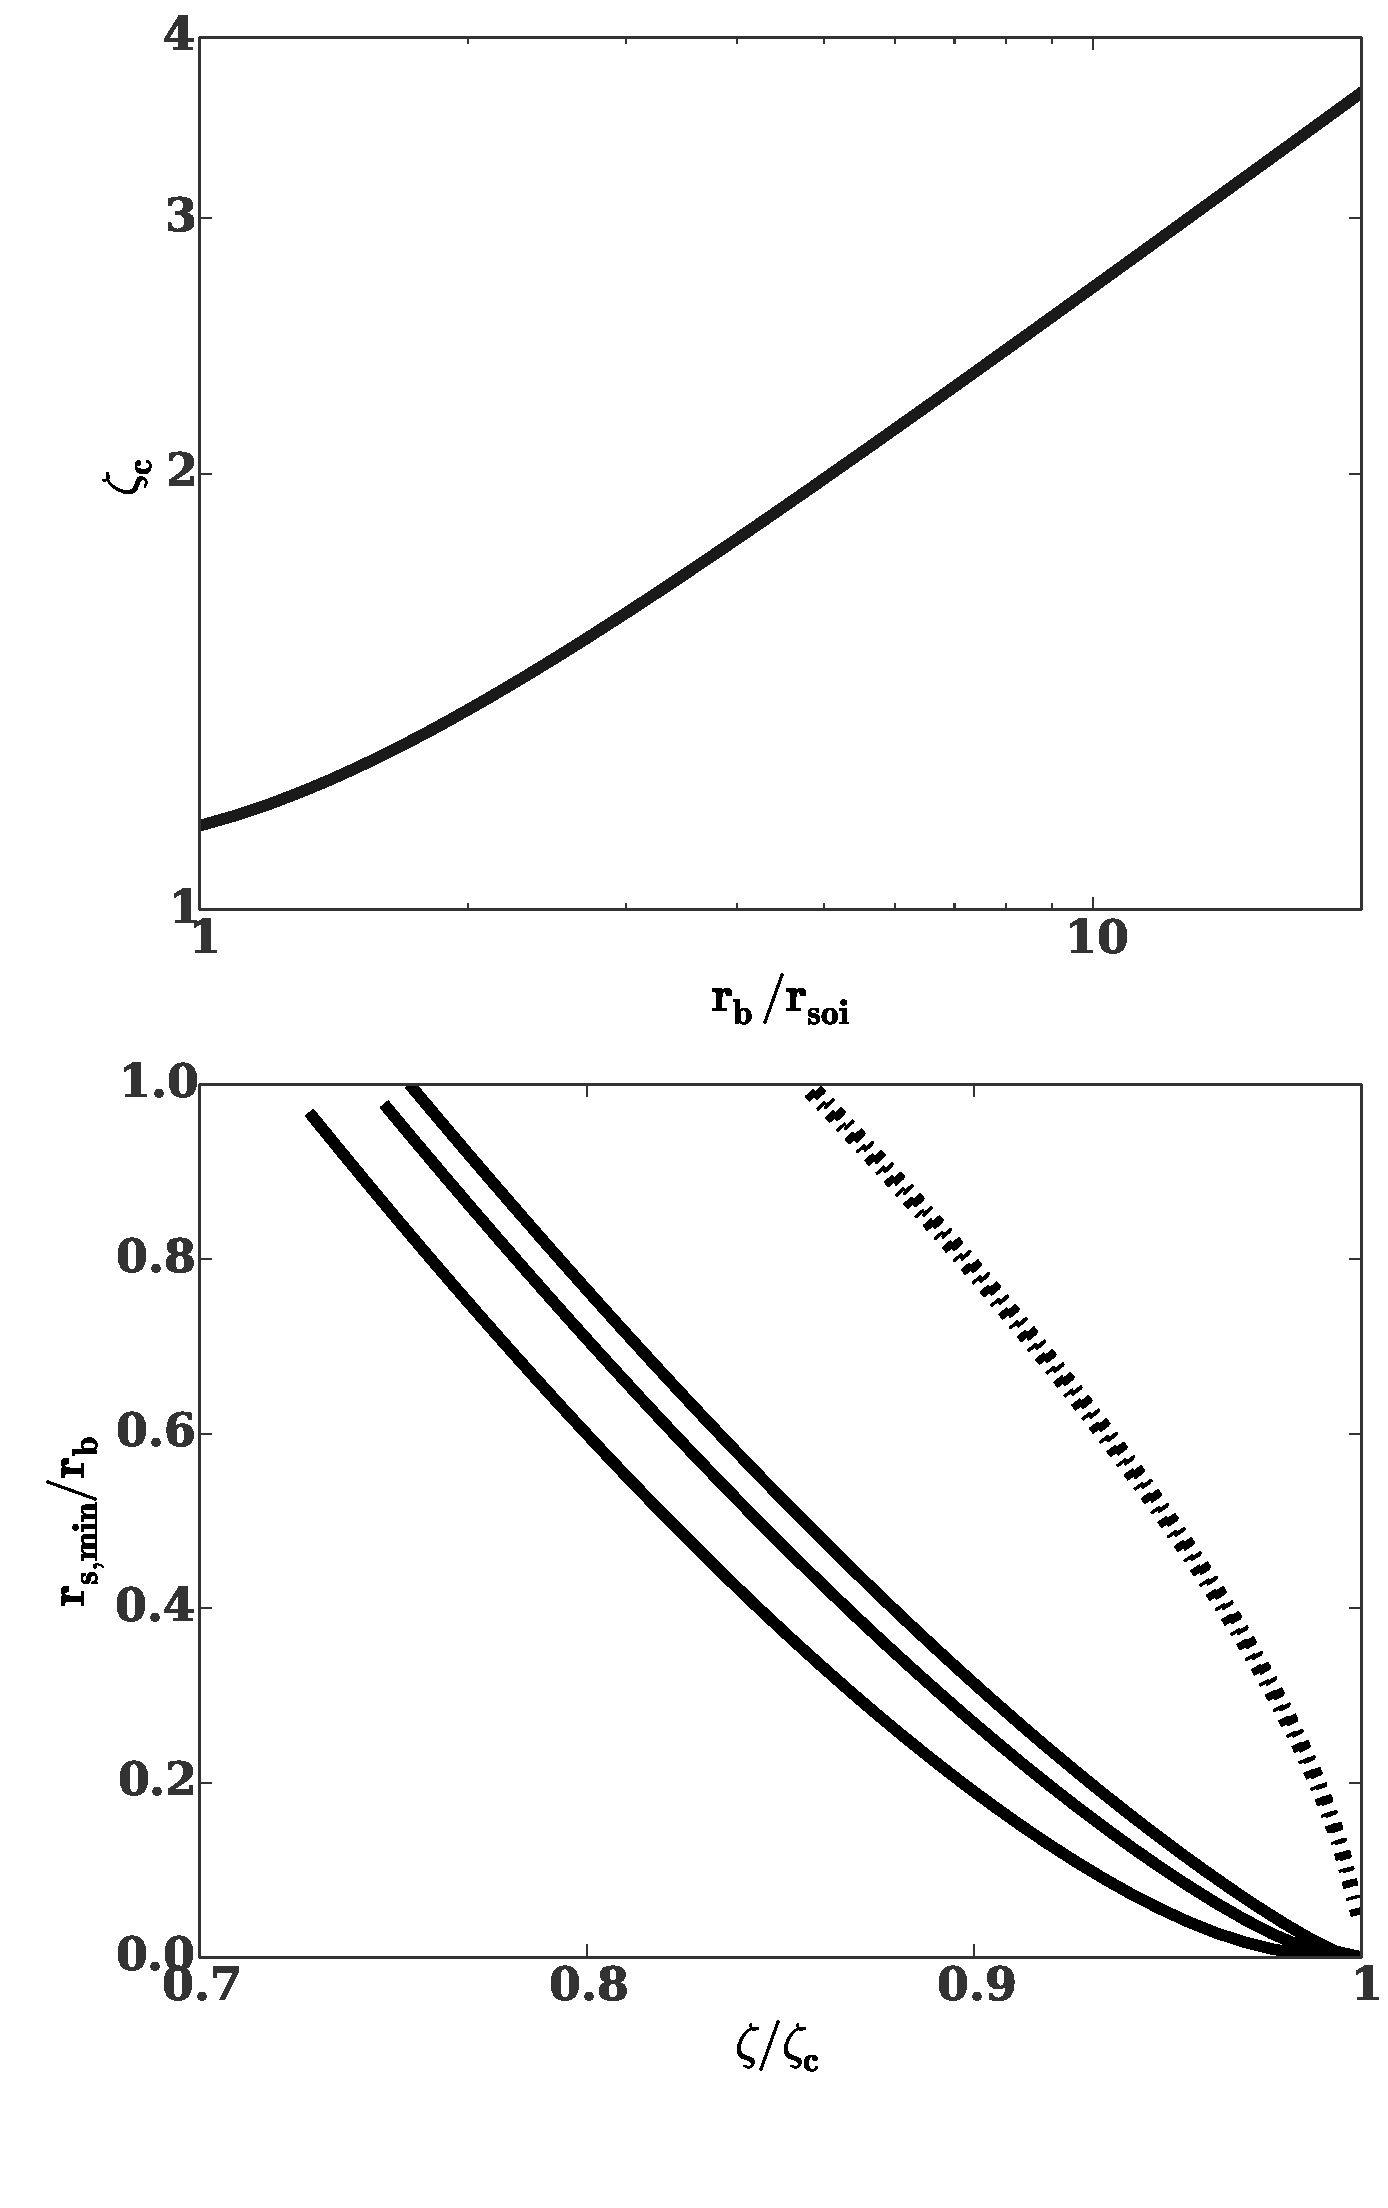
\includegraphics[width=\columnwidth]{zetaCrit.pdf}
\caption{\label{fig:zetaCrit} {\emph Top panel:} Critical
  $\zeta_c=\sqrt{v_w^2+\sigma_0^2}/\sigma_0$. If $\zeta<\zeta_c$ outflows are
  only possible if the ratio of the stagnation radius to the influence
  radius exceeds a minimum value. Plotted as a function of the ratio
  of the break radius to the influence radius ($\rb/\rsoi$) {\emph Bottom
    Panel:} Mininmum value for ratio of the stagnation radius to the
  influence radius, $\rs/\rsoi$ for core galaxies ($\Gamma=0.1$)
  derived by requiring enthalpy of the gas to remain positive out to
  the break radius $\rb$. This is calculated numerically from
  equation~\eqref{eq:enthAnal}. The x-intercept of each curve
  corresponds to the critical $\zeta_c$}
\end{figure}


%%% Local Variables: 
%%% mode: latex
%%% TeX-master: "ms"
%%% End: 


  \section{Analytic model for dependence of wind heating $\vwO^{\star}$ on stellar age}
\label{app:windheat}
% If we assume that a stellar population forms
% impulsively in the distant pass with IMF $\mu(m_*)$(with minimum mass
% $m_0$ and maximum mass $m_1$), then the surviving mass fraction at any
% future time $t$ is given by
% \begin{equation}
% f(t) =\frac{ \int_{m_0}^{m_{\rm T}(t)} m_* \mu(m_*) dm_* }{ \int_{m_0}^{m_1} m_* \mu(m_*) dm_* },
% \end{equation}
% where the main sequence turnoff mass is approximately
% \begin{equation}
% m_{\rm T}(t) \approx 2.5M_\odot~ \left( \frac{t}{10^9~{\rm yr}} \right)^{-0.4}.
% \end{equation}
% For a Salpeter IMF $\mu(m_*) \propto m_*^{-2.35}$ with $m_0=0.1M_\odot$ and $m_1=100M_\odot$,
% \begin{equation}
% f_{\rm Sal}(t) = 1.098 - 0.490 \left(\frac{t}{10^{10}~{\rm yr}} \right)^{0.14}
% \end{equation}
% {\bf NCS: we should probably use a Kroupa/Chabrier IMF, but this gets the ball rolling.}
% If we approximate post-main sequence evolution as instantaneous and define $\lambda(\Mstar)$ as the fractional mass lost during all stages of stellar evolution, then the mass loss rate density
% \begin{equation}
% q(t) = \frac{\rho_*}{\bar{m}_*} \lambda(m_{\rm T}(t)) m_{\rm T}(t) \frac{df}{dt},
% \end{equation}
% where the mean stellar mass $\bar{m}_* = \int_{m_0}^{m_{\rm T}(t)} \Mstar\mu(\Mstar)d\Mstar \approx 0.3 M_\odot$.  Further approximating $\lambda(\Mstar)=0.5$, and using the Salpeter IMF once more, gives
% \begin{equation}
% q(t) = \frac{\rho_*}{10^{10}~{\rm yr}} \times 0.11 \left(\frac{t}{10^{10}~{\rm yr}} \right)^{-1.26}.
% \end{equation}
% This is a specific, time-dependent definition of $\eta(t) (=0.11(t/t_{\rm h})^{-1.26})$; if we consider different star formation scenarios (for example, continuous star formation) or different IMFs, it will change.  Once these free parameters are specified, however, we can answer an important question: do young stellar populations increase or decrease the SMBH feeding rate $\dot{M}$?  Clearly, $\eta(t)$ is larger for young stellar populations, but these stars also have high wind velocities that diminish the stagnation radius.  Crudely approximating $v_{\rm w}=75~{\rm km~s}^{-1}$ for $m_{\rm T} < 10M_{\odot}$ and $v_{\rm w}=3000~{\rm km~s}^{-1}$ for $m_{\rm T} > 10M_{\odot}$ (motivated by the transition from dust-driven wind loss on the AGB to line-driven wind loss from Wolf-Rayet stars), we can employ the relation $\dot{M} \propto \eta(t) r_{\rm s}^{2-\Gamma}\propto \eta(t) v_{\rm w}^{-4+2\Gamma}$ (where $\rho_* \propto r^{-\Gamma}$) to determine the impact of stellar ``youth'' on SMBH feeding rates.
% {\bf AG:As I previously mentioned this discussion of the eta is not
%   quite correct...}
% \begin{figure}
% 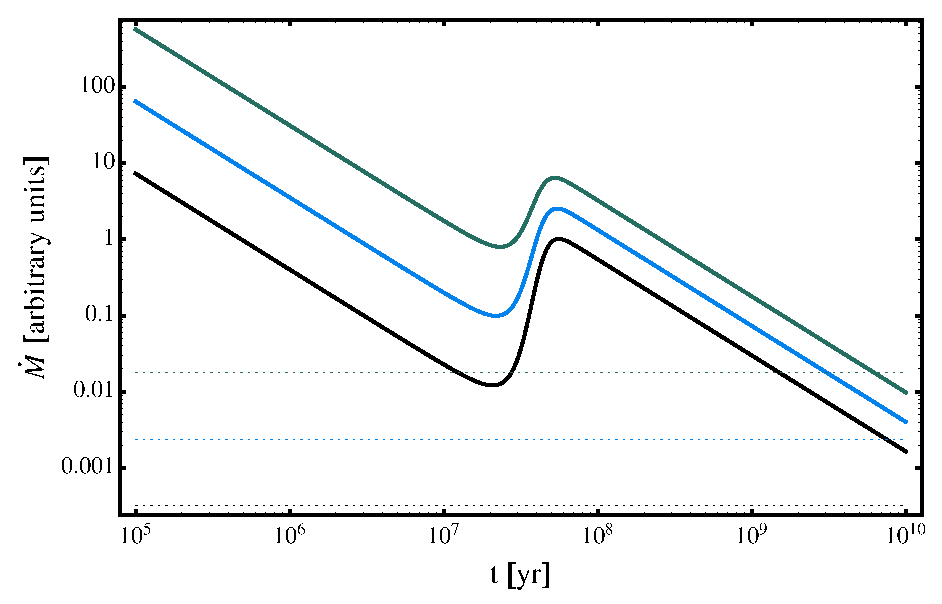
\includegraphics[width=\columnwidth]{NickPlot.eps}
% \caption{\label{NickPlot} SMBH feeding rates $\dot{M}=\eta(t) \times \Mstar(r_{\rm s})$, in arbitrary units.  The green, blue, and black curves are for galaxies with $\Gamma$ values of $0.1$, $0.5$, and $0.9$, respectively.  Solid curves represent impulsive-mode star formation, while dotted curves represent continuous-mode star formation. {\bf NCS: I think these old continuous curves are wrong, need to revise}}
% \end{figure}

% In Fig. \ref{NickPlot} we plot $\dot{M}$, in arbitrary units, as a
% function of time, for three different stellar density profiles $\Gamma
% = \{1.1, 1.5, 1.9\}$ (which are normalized to have the same mass at an
% influence radius $r _{\rm soi}=10~{\rm pc}$ around a $10^7M_\odot$
% SMBH).  We parametrize the wind velocity as
% \begin{equation} \frac{v_{\rm w}}{3000 ~\rm
% km~s^{-1}}=520-495\tanh\left( \frac{t-10^{7.5}~{\rm yr}}{10^{7}~{\rm
% yr}}\right). \label{NickV1}
% \end{equation} This counts Type II SNe heating as ``winds;'' if
% instead we are in the portion of parameter space where $r_{\rm II}$ is
% very large, then we use the alternate parametrization
% \begin{equation} \frac{v_{\rm w}}{3000 ~\rm
% km~s^{-1}}=520-495\tanh\left( \frac{t-10^{7}~{\rm yr}}{10^{6.5}~{\rm
% yr}}\right), \label{NickV2}
% \end{equation} which only allows short lived Wolf-Rayet stars to
% contribute to the high-heating mode.  The ``impulsive burst'' mode of
% star formation produces large ($\sim 10$) differences between the
% three $\dot{M}$ curves at early times, when $r_{\rm s}$ is small, but
% smaller ($\sim 3$) differences at late times, when $r_{\rm s}$ is
% large.  We also plot, as dotted curves, a simple model for the
% ``continuous'' mode of star formation, where mass loss is calculated
% as $\bar{\eta} = \int\eta(t)dt/t_{\rm h} \approx 4$ and an average
% energy injection in the wind is calculated as $\bar{v_{\rm
% w}^2}=\int\eta(t)v_{\rm w}^2(t)dt/\bar{\eta} \approx (800~{\rm
% km~s}^{-1})^2$.  Interestingly, the continuous mode of star formation
% produces small differences from late-time $\dot{M}$ seen in cusp
% galaxies with impulsive star formation; however, continuous mode star
% formation decreases late-time $\dot{M}$ by an order of magnitude
% relative to impulsive star formation in core galaxies.  {\bf NCS: I
% think this old discussion of MDot in the continuous limit is wrong,
% need to revise}

The energy and mass injection from stellar winds will be the sum ofthe
contributions from main sequence and post-main sequence (PMS) stars.
For an impulsively formed stellar population of age $t$, the mass
injection rate per unit stellar mass,$\dot{\bar{m}}(t)$, and  the energy
injection rate per unit stellar mass, $\dot{\bar{e}}(t)$,  will be given by

\begin{align} 
  \dot{\bar{m}}(t) &= \frac{\Delta M(t) \mu(M_{\rm TO}(t))
    \left|\dot{M}_{\rm TO}(t)\right| + f_{\rm MS} \int_{m_0}^{m_{\rm
        T}(t)}
    \dot{m}(\Mstar, t) \mu(\Mstar) {\rm d}\Mstar }{\bar{m}_*}\\
  \dot{\bar{e}}(t) &=\dot{e}_{\rm TO}(t)+ f_{\rm MS} \int_{m_0}^{m_{\rm T}(t)}
  \frac{\vw^2(\Mstar, t) \dot{m}(\Mstar, t) \mu(\Mstar) {\rm d}\Mstar}{\bar{m}_*}.
  \label{eq:edotImp}
\end{align} 

The first terms in each expression above correspond to the
contributions from PMS stars, while the second terms correspond to the
contributions from main sequence stars. The main sequence winds are a
small fraction of the mass, and they may be not be thermalized and
mixed with the rest of the injected gas. Thus, we include a
thermalization efficiency, $ 0\le f_{\rm MS}\le 1$, in
equation~\eqref{eq:edotImp}. Throughout this paper we set $f_{\rm
  MS}=1$. 

We assume a Salpeter IMF $\mu(\Mstar)\sim M^{-2.35}$, truncated at $0.1
\Msun$ on the low mass end and at $100 \Msun$ on the high mass
end. The corresponding mean stellar mass, $\bar{m}_*$ is 0.35 $\Msun$.

For the turnoff mass, $M_{\rm TO}$, we take the following fitting
formula 

\begin{align}
\log(M_{\rm TO})=0.24 + 0.068 x^2-0.34 x+4.76 e^{-4.58 x},
\end{align}

where $x=\log(t/10^9 {\rm years})$ and $M_{\rm TO}$ is in units
$\Msun$. This fit is designed to reproduce the results in 
Table 9 of \citet{MaederMeynet:1987a} and then asymptotes to the fit
for $M_{\rm TO}$ given in equation (9) of \citet{CiottiOstriker:2007a}
for intermediate and late times ($t \gsim 10^8$ years).

For $\Delta M(t)$ we use equation (10) from \citet{CiottiOstriker:2007a}

\begin{align}
\Delta M=
\begin{cases}
0.945 M_{\rm TO}-0.503 & M_{\rm TO} < 9 \Msun\\
 M_{\rm TO}-1.4 \Msun &  M_{\rm TO} \ge 9 \Msun
\end{cases}
\end{align}

To estimate the mass loss from main sequence stars
$\dot{m}(\Mstar, t)$,
we use equation 4 \citet{SchroderCuntz:2005a}\footnote{This
  prescription is a generalization of the Reimers' mass loss law. This
expression is derived assuming the stellar wind results from the
turbulent overflow of moaterial in the chromosphere or underneath it.} {\bf AG:
  unfortunately this is not really meant for MS stars...}

\begin{align}
  \dot{m}(\Mstar)=8 \times 10^{-14} \frac{L_* R_*}{\Mstar}
  \left(\frac{T_{\rm eff}}{\rm 4000 K}\right)^{3.5}
  \left(1+\frac{g_{\odot}}{4300 g_*}\right) \Msun \pyear,\
\end{align}

where  $R_*$, $L_*$, $T_{\rm eff}$ and $g_*$ are the stellar radius,
luminosity, effective and surface gravity respectively. $g_{\odot}$ is
the stellar surface gravity. To calculate $R_*$ and $L_*$ we use the
following scaling relations (taken from Kippenhann and Weygert Figures
22.2 and 22.3).

\begin{align}
L_*=
\begin{cases}
L_{\odot} (\Mstar/\Msun)^{3.2} & \Mstar > \Msun \\
L_{\odot} (\Mstar/\Msun)^{2.5} & \Mstar \le \Msun
\end{cases}
\end{align}

\begin{align}
r_*=
\begin{cases}
R_{\odot} (\Mstar/\Msun)^{0.57} & \Mstar > \Msun \\
R_{\odot} (\Mstar/\Msun)^{0.8} & \Mstar \le \Msun
\end{cases}
\end{align}


To get a handle on $\dot{e}_{\rm TO}(t)$, we use the results from
\citet{VossDiehl+:2009a} who use a population synthesis code to
simulate the mass and energy injection into the ISM from an OB
association. For the first $\sim 10$ Myr the energy injection will
come from energetic Wolf-Rayet star winds. The energy injection rate
per massive star ($\Mstar>8 \Msun$), $\dot{\mathcal{E}} (t)$, from
stellar winds is plotted in the top panel of their Figure 7 and is
well fit {\bf AG: A little more detail here...} by

\begin{align}
\dot{\mathcal{E}} (t)=
\begin{cases}
  1.3 \times 10^{36} {\rm ergs/s} & t<4 \times 10^6 {\rm years}\\
  1.3  \times 10^{36} {\rm ergs/s} \left(\frac{t}{4 \times  10^6}\right)^{-3.73} & t \ge 4 \times 10^6 {\rm years}.
\end{cases}
\label{eq:voss}
\end{align}

 $\dot{e}_{\rm TO}(t)$ is related to $\dot{\mathcal{E}}$  via 

\begin{align}
\dot{e}_{\rm TO}(t)=f_{8} \dot{\mathcal{E}} / \bar{m}_*,
\label{eq:eto}
\end{align}

where $f_{8}$ is the fraction of the stellar population with
$\Mstar>8 \Msun$. $f_8=2.6 \times 10^{-3}$ for our assumed Salpeter
IMF.  Equation~\eqref{eq:voss} and~\eqref{eq:eto} will be valid onlyfor $t
\lsim 10$ Myr. However, the turnoff contribution will become extremely
energetically subdominant at later times as far slower dust-driven
winds come to dominate the energy budget {\bf AG: Nick check--is the
  preceding sentence accurate}

We calculate the wind velocity for main sequence winds $v_w (\Mstar,
t)$ using...{\bf AG:Current just use the value for the sun~430 km/s
  replace with the real prescription we end up using.}

The effective wind velocity in the impulsive limit may then be written
as 

\begin{align}
\bar{v}_w(t)=2 \dot{\bar{e}}(t)/\dot{\bar{m}}(t)
\label{eq:vwImp}
\end{align}

We plot $\bar{v}_w$ in Figure~\ref{fig:vwImp}.

\begin{figure}
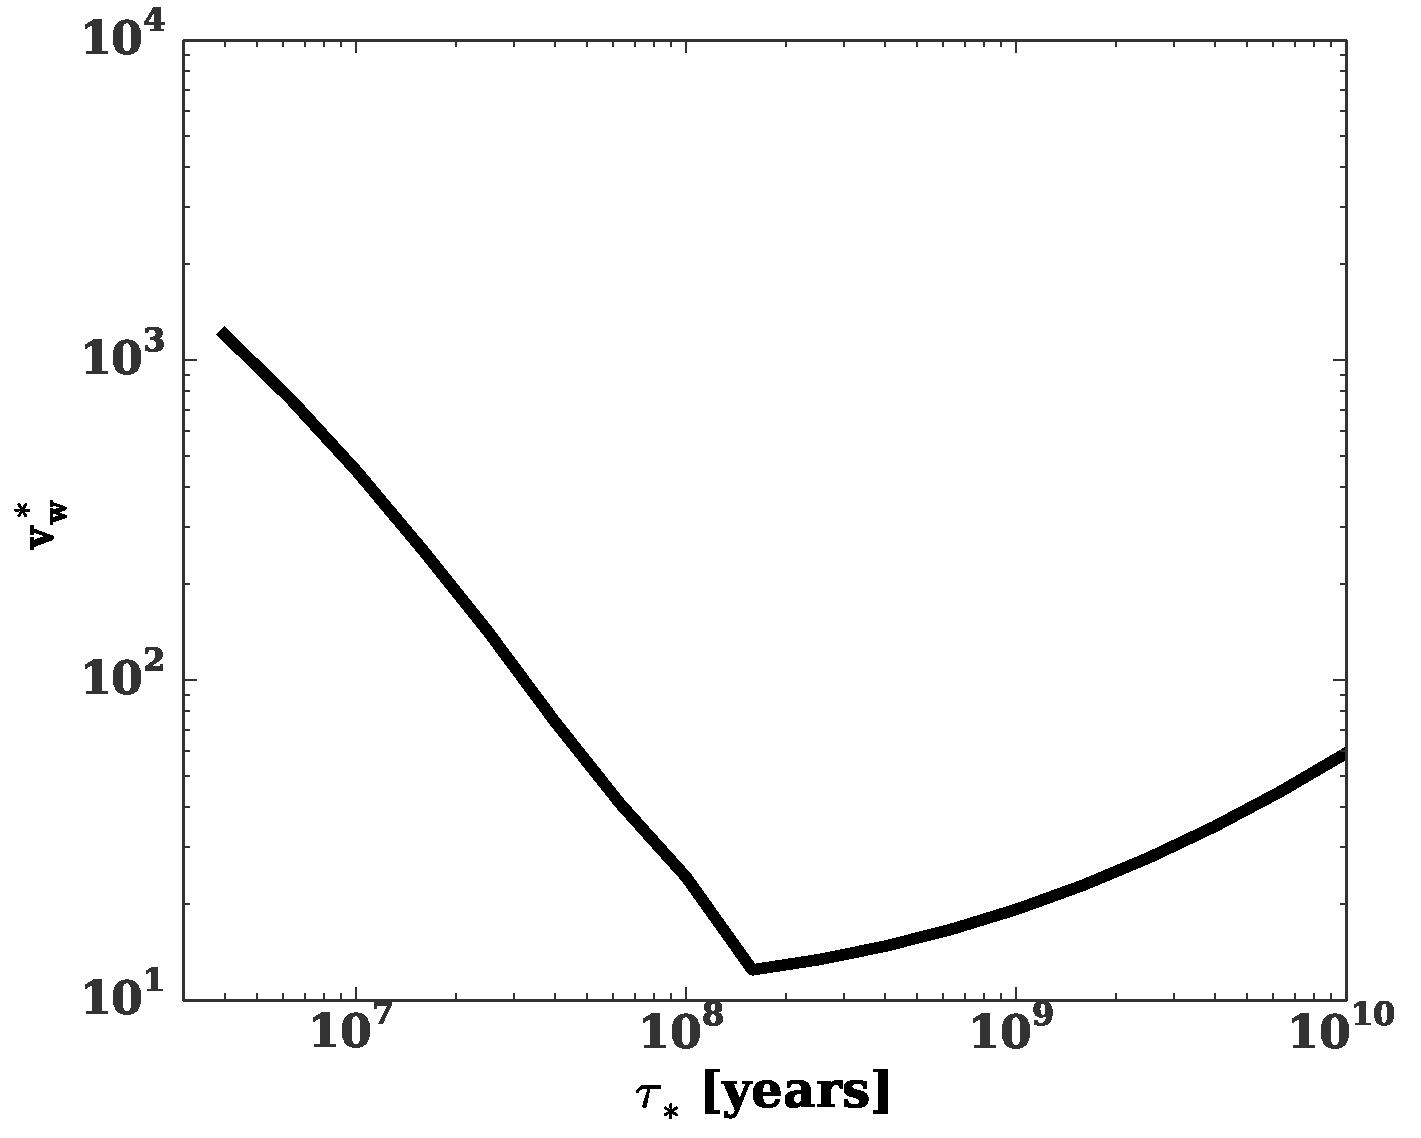
\includegraphics[width=\columnwidth]{vwImp.pdf}
\caption{\label{fig:vwImp} The effective $\vw$ from stellar winds from
  a stellar population formed in a starburst $t$ years ago.}
\end{figure}

We can then use these integrated quantities to determine the effective
$V_w$ for arbitrary star formation histories. For a stellar population
with star formation rate $S(t)$ 

\begin{align} 
  \dot{M}(t) &= \int_0^t S(t_1) \dot{\bar{m}}(t-t_1){\rm
      d}t_1\\
  \dot{E}(t) &= \int_0^t S(t_1) \dot{\bar{e}}(t-t_1){\rm
      d}t_1\\
  V_w^2(t) &=2 \dot{E}(t)/\dot{M}(t)
\end{align}

\begin{figure}
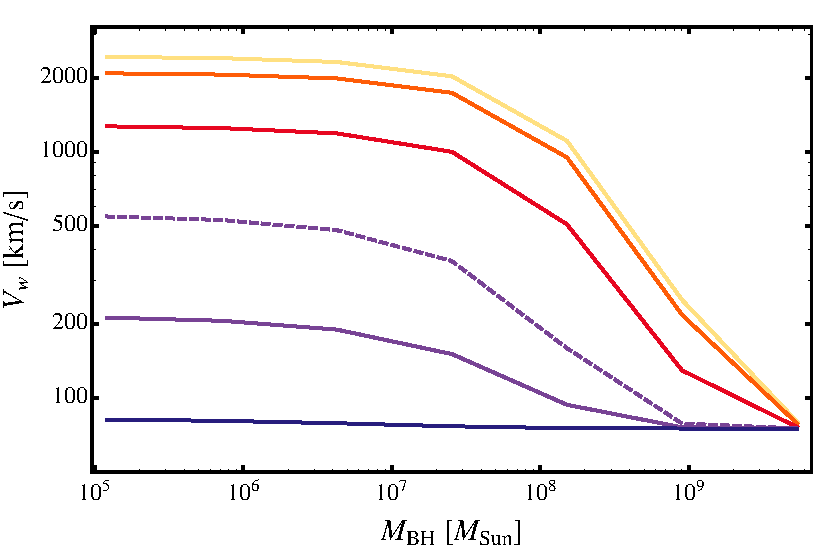
\includegraphics[width=\columnwidth]{vw.pdf}
\caption{\label{NickPlot2} Effective wind velocities $V_{\rm w}$ for
different $S(t)$.  The yellow and orange curves are the Moster SF
histories, with and without Type II SNe, respectively.  The red,
purple, and blue curves are Moster SFs convolved with a $\sin^2(t)$
function normalized to $10^7$, $10^8$, and $10^9$ yr fluctuations,
respectively.  These solid curves lack SN, but the dashed purple curve
possesses it.  Effective $V_{\rm w}$ is strongly diminished when the
variability timescale is greater than $\sim$ twice the duration of
high-velocity winds.}
\end{figure}

We show $V_{\rm W}$ for different star formation histories in
Fig. \ref{NickPlot2}.  In particular, we use Eqs. 17-20 from Moster et
al and the $M_{\rm BH}-M_{\rm halo}$ relation from Bandara et al {\bf
(NCS: add real refs)} to define $S(t)$ for particular galaxies.  It
seems that ``bumpy'' SF histories severely diminish $V_{\rm w}$ if the
timescale for SF variability is a factor of a few or more greater than
the duration of high-velocity winds (either 10 or 40 Myr).

%%% Local Variables: 
%%% mode: latex
%%% TeX-master: "ms"
%%% End: 


  \footnotesize{
    \bibliographystyle{mn2e}
    \bibliography{master}
  }
\end{document}
